% Ensure that arXiv processes this as PDF.
\pdfoutput=1

\documentclass{book}
\usepackage{mylhs2tex}
\usepackage{natbib}
\usepackage{rotating}
\usepackage{comment}
\bibliographystyle{abbrvnat}
% Emacs, this is -*- latex -*-!
\usepackage{natbib}
\usepackage{rotating}
\usepackage{amsmath}
\usepackage{comment}
\usepackage[shortlabels]{enumitem}
\usepackage[T1]{fontenc}
\usepackage[utf8]{inputenc}
\usepackage{xparse}
\usepackage{microtype}

\usepackage{subcaption}

% This package allows hyphenation of compound words. Use \-/
% instead of - as hyphen to allow hyphenation elsewhere. Use \=/
% to additionally specify that hyphenation right after the dash
% is forbidden. However, this package with this setting redefines
% \- and \=!

%\usepackage[shortcuts]{extdash}

\usepackage{etoolbox} %For newtoggle
\newtoggle{todos}

% Show empty space at page ends, to ease squeezing space.
% Should remove before submission.
%\raggedbottom

% For submission. These settings shouldn't be altered.
\togglefalse{todos}
% \toggletrue{todos}
\allowdisplaybreaks[1]
% For development, feel free to tune if needed.
% Allow reasonable looks without huge cost, during development.
%   \allowdisplaybreaks[1]
%   %\sloppy

% Introduce environment oldSec for material which we commented out but might
% still have bits to save:
\excludecomment{oldSec}
% Replace the above line with:
%\includecomment{oldSec}
% to comment those sections back in.
\newenvironment{optionalproof}{\begin{proof}}{\end{proof}}
\newenvironment{optionallemma}{\begin{lemma}}{\end{lemma}}

% Emacs, this is -*- latex -*-!
\usepackage[scaled=0.88]{beramono} % http://wbillingsley.blogspot.de/2008/06/latex-monospace-bold-computer-modern.html
\usepackage{array}
\usepackage{booktabs}
\usepackage{mathpartir}

\usepackage[amsmath,thmmarks,amsthm]{ntheorem}
\usepackage{thmtools}
\usepackage{thm-restate}
% Load hyperref as last package
% (http://www.tex.ac.uk/cgi-bin/texfaq2html?label=hyperdupdest), except for
% bookmark (which would otherwise load hyperref with other options).
\usepackage[unicode=true]{hyperref}
\usepackage{bookmark}

% Comments
\iftoggle{todos}{%
\usepackage{amssymb}
\usepackage{stmaryrd}
\usepackage{xcolor}
\newcommand{\mynote}[2]{
  \textcolor{red}
  {
  {\bfseries\sffamily\scriptsize#1}
  {\small$\blacktriangleright$\textsf{\emph{#2}}$\blacktriangleleft$}}}
}{%
\newcommand{\mynote}[2]{}
}

\newcommand{\todo}{\mynote}

\newcommand{\tr}{\todo{TR}}
\newcommand{\pg}{\todo{PG}}
\newcommand{\ko}{\todo{KO}}
\newcommand{\yc}{\todo{YC}}
\newcommand{\chk}{\todo{CK}}
\newcommand{\mei}{\todo{ME}}
\newcommand{\rmi}{\todo{RM}}

% Allow using λ in section headers and having it show in PDF bookmarks.
% http://tex.stackexchange.com/a/142906/1340
\usepackage{newunicodechar}
\newunicodechar{λ}{\texorpdfstring{\ensuremath{\lambda}}{λ}}
\DeclareRobustCommand{\TitleLambda}{λ}
\newunicodechar{⊕}{\texorpdfstring{\ensuremath{\oplus}}{⊕}}


\usepackage{amsthm,fixfoot}

\usepackage{listings}
% Hey Emacs this is -*- latex -*-
% From http://tihlde.org/~eivindw/latex-listings-for-scala/
% "define" Scala
%Keyword list taken from the scaladoc definition.
\lstdefinelanguage{scala}{
  morekeywords={%
	  abstract,case,catch,class,def,do,else,extends,%
	  false,final,finally,for,forSome,if,implicit,import,lazy,%
	  match,new,null,object,override,package,private,protected,%
	  return,sealed,super,this,throw,trait,true,try,type,%
	  val,var,while,with,yield},
  otherkeywords={=>,<-,<\%,<:,>:,\#,@,scala>},
  sensitive=true,
  morecomment=[l]{//},
  morecomment=[n]{/*}{*/},
  morestring=[b]",
  morestring=[b]',
  morestring=[b]"""
}[keywords,comments,strings]

% activate the language and predefine settings
\lstset{%
    language=Scala,%
    tabsize=2,%
    basicstyle=\ttfamily,%
    commentstyle=\itshape,%
    keywordstyle=\bfseries,%
    identifierstyle=,% nothing
    stringstyle=\ttfamily, % typewriter type for strings
    mathescape=true,%
    escapechar=£,%
    numberstyle=\tiny,%
}

%Setup whitespace in listings
\lstset{%
%columns=fullflexible,		% enable kerning, lose column alignment.
showstringspaces=false, %
breaklines=false,
breakatwhitespace=false,
breakautoindent=false,
keepspaces
%keepspaces was described at: http://tex.stackexchange.com/questions/41954/listings-bug-space-after-literate-replacement-lost-with-spaceflexible-fullflexi
}

\newcommand{\codesize}{}

% Command for in-text code snippets, if needed.
\newcommand{\code}{%
    \lstinline[basicstyle=\codesize\ttfamily]}

% I use ^ as the only decent alternative - not-ASCII characters don't work in this setup (probably because of UTF-8).}
% literate programming: replace some operators by nicer equivalents.
%{==}{{$\equiv$}}1 {!=}{{$\neq$}}1
\lstset{literate={{<-}{{$\gets$}}1 {<=}{{$\leq$}}1 {>=}{{$\geq$}}1 { => }{{$\Rightarrow$}}1 { -> }{{$\rightarrow$}}1 {...}{{\ldots} }2}}


% Macros specific to this paper project

\providecommand{\nocaptionrule}{} %Hack for non-SIGPLAN formats.
% \DeclareMathOperator{\ExpWrap}{Lift}
\newcommand{\ExpWrap}{\mathit{Lift}}
%\newcommand{\LoS}{SCQL} % Scala Collection Query Language
%\newcommand{\LoS}{Squopt} % Scala Query Optimizer
\newcommand{\LoS}{\textsc{SQuOpt}} % Scala Query Optimizer % Try to get Squaw?
\newcommand{\LoSDef}{\LoS, the Scala QUery OPTimizer}
%\newcommand{\LoS}{\textsc{Squash}}
%\newcommand{\LINQ}{LINQ}
\newcommand{\LINQ}{\textsc{Linq}}

\hypersetup{breaklinks=true, pdfborder={0 0 0}}

%\newcommand{\textsubscr}[1]{\ensuremath{_{\scriptsize\textrm{#1}}}}
%\setlength{\parindent}{0pt}
%\setlength{\parskip}{6pt plus 2pt minus 1pt}
%\setlength{\emergencystretch}{3em}  % prevent overfull lines
%\setcounter{secnumdepth}{0}

\newcommand{\intersect}{\wedge}
\providecommand{\IEEEPARstart}[2]{#1#2}

\newcommand{\smartParagraph}[1]{\textbf{#1}}

% Macros specific to this paper project

% Macros for terms, types and values
%
% Naming Convention:
%   \UPPERCASE -- single keyword
%   \Mixed     -- term constructor
%
% All term constructors have a starred form to add parentheses.
%
% Example:
%
%   \App{\Lam*{x}{\Var{x}}}{\Lit{42}}  gives  (λx.x) 42

% Consider using.
%   \newcommand{\eqdef}{\ensuremath{=_{\mathit{def}}}}

\usepackage{mathtools}
\newcommand\validfromto[4]{#3 \;\rhd\; #2 \xhookrightarrow{#1} #4}
\newcommand\correctdt[2]{#1 \;\rhd \; #2}
\DeclareMathAlphabet{\mathcal}{OT1}{pzc}{m}{it}

\newcommand{\Keyword}[1]{\textbf{#1}}
\newcommand{\Term}[1]{\Varid{#1}}

\newenvironment{equational}{
\def\commentbegin{\quad\{\ }
\def\commentend{\}}
}{}

% Lists

\NewDocumentCommand{\List}{sm}{\Parens#1{\overline{#2}}}

% Helper for optional subscripts and superscripts

\NewDocumentCommand{\Index}{sm}{\IfValueTF{#2}{\IfBooleanTF{#1}{^}{_}{#2}}{}}

% \DIFF          for   ⊖
% \Diff{u}{v}    for   u ⊖ v

% Deprecated:
% \APPLY         for   ⊕
% \Apply{dv}{v}  for   v ⊕ dv
%
% New:
% \UPDATE        for   ⊕
% \Update{v}{dv} for   v ⊕ dv.
\NewDocumentCommand{\DIFF}{o}{\ominus\Index{#1}}
\NewDocumentCommand{\UPDATE}{o}{\oplus\Index{#1}}
%Deprecated alias.
\let\APPLY\UPDATE

\NewDocumentCommand{\Upd}{sm}{\Parens#1{#2 \UPDATE \D #2}}

\NewDocumentCommand{\Diff}{somm}{\Parens#1{#3 \DIFF[#2] #4}}

\NewDocumentCommand{\Update}{somm}{\Parens#1{#3 \UPDATE[#2] #4}}
% Deprecated variant. Beware of the copy and paste!
\NewDocumentCommand{\Apply}{somm}{\Parens#1{#4 \UPDATE[#2] #3}}

\NewDocumentCommand{\WideDiff}{somm}{\Parens#1{#3 \;\;\DIFF[#2]\;\; #4}}
\NewDocumentCommand{\WideApply}{somm}{\Parens#1{#4 \;\;\APPLY[#2]\;\; #3}}

\NewDocumentCommand{\NILC}{}{\mathbf{0}}
\NewDocumentCommand{\NilC}{om}{\NILC_{#2}}

\NewDocumentCommand{\ChangeStruct}{m}{\widehat{#1}}
\NewDocumentCommand{\chs}{m}{\ChangeStruct{#1}}

%http://tex.stackexchange.com/a/163831/1340
\usepackage{stackengine}
\NewDocumentCommand{\Doe}{}{\mathrel{\stackon[1pt]{$=$}{$\scriptscriptstyle\Delta$}}}
%{\ensuremath{\overset{\scriptscriptstyle\GD}{=}}}
%{\triangleq}

\NewDocumentCommand{\MAP}{}{\Term{map}}

\NewDocumentCommand{\Xs}{}{\Term{xs}}
\NewDocumentCommand{\Ys}{}{\Term{ys}}
\NewDocumentCommand{\Zs}{}{\Term{zs}}
\NewDocumentCommand{\Program}{}{\Term{grand\_total}}
\NewDocumentCommand{\ProgramBody}{}{\Lam{\Xs}{\Lam{\Ys}{\FOLD~(+)~0~(\Merge\Xs\Ys)}}}
\NewDocumentCommand{\Derivative}{}{\Term{dgrand\_total}}
\NewDocumentCommand{\Output}{}{\Term{output}}

\NewDocumentCommand{\DXs}{}{\Term{dxs}}
\NewDocumentCommand{\DYs}{}{\Term{dys}}
\NewDocumentCommand{\DZs}{}{\Term{dzs}}
\NewDocumentCommand{\DOutput}{}{\Term{doutput}}

% Semantic brackets
% \mean t       for   ⟦t⟧
% \mean[\Gr]t   for   ⟦t⟧ ρ
% \mean*[\Gr]t  for   (⟦t⟧ ρ)
\NewDocumentCommand{\mean}{soomo}{\Parens#1{%
\left\llbracket\,#4\,\right\rrbracket\IfNoValueTF{#5}{}{^{#5}}\IfNoValueTF{#2}{}{\;#2}\IfNoValueTF{#3}{}{\;#3}}}

% Environment update
% \update x v \Gr   for   ρ[x ↦ v]
% \update* x v \Gr  for   (ρ[x ↦ v])
\NewDocumentCommand{\update}{smmm}{\Parens#1{#4[#2\mapsto#3]}}

% \D x   for  dx
%
% Warning: \D x typesets dx as a single word, unlike dx.
% See discussion of mathit in, e.g.,
% http://tex.stackexchange.com/a/58108/1340.
\NewDocumentCommand{\D}{m}{\Term{d#1}}

% \Old f for  f_old
\NewDocumentCommand{\Old}{m}{#1_{\textrm{old}}}
\NewDocumentCommand{\New}{m}{#1_{\textrm{new}}}

\NewDocumentCommand{\APPFun}{}{\Keyword{app}}
\NewDocumentCommand{\IF}{}{\mathop{\Keyword{if}}}
\NewDocumentCommand{\THEN}{}{\mathbin{\Keyword{then}}}
\NewDocumentCommand{\ELSE}{}{\mathbin{\Keyword{else}}}
\NewDocumentCommand{\TRUE}{}{\Keyword{true}}
\NewDocumentCommand{\FALSE}{}{\Keyword{false}}
\NewDocumentCommand{\BAG}{}{\mathop{\Keyword{Bag}}}
\NewDocumentCommand{\MERGE}{}{\Term{merge}}
\NewDocumentCommand{\NAT}{}{\Keyword{Nat}}
\NewDocumentCommand{\INT}{}{\Keyword{Int}}
\NewDocumentCommand{\BOOL}{}{\Keyword{Bool}}
\NewDocumentCommand{\EVAL}{}{\mathcal{Eval}}
\NewDocumentCommand{\DOM}{}{D}
\NewDocumentCommand{\NEGATE}{}{\Term{negate}}
\NewDocumentCommand{\CHANGE}{o}{\Delta\Index{#1}}
\NewDocumentCommand{\BASE}{}{\mathop{\Keyword{Base}}}

\NewDocumentCommand{\Parens}{mm}{\IfBooleanTF#1{\left(#2\right)}{#2}}

\NewDocumentCommand{\Fun}{smm}{\Parens#1{#2 \to #3}}
\NewDocumentCommand{\Base}{sO{}}{\Parens#1{\App\BASE{#2}}}
\NewDocumentCommand{\Bag}{sO{}}{\Parens#1{\IfValueTF{#1}{\App\BAG{#2}}{\BAG}}}
\NewDocumentCommand{\Nat}{s}{\Parens#1{\NAT}}
\NewDocumentCommand{\Int}{s}{\Parens#1{\INT}}

\NewDocumentCommand{\Set}{m}{\left\lbrace\left\lbrace#1\right\rbrace\right\rbrace}

\NewDocumentCommand{\APP}{}{\;}
\NewDocumentCommand{\App}{smm}{\Parens#1{#2\;#3}}
\NewDocumentCommand{\Lam}{smm}{\Parens#1{\lambda#2 \rightarrow \ #3}}
\NewDocumentCommand{\Var}{sm}{\Parens#1{#2}}
\NewDocumentCommand{\Const}{sm}{\Parens#1{#2}}
\NewDocumentCommand{\Lit}{sm}{\Parens#1{#2}}
\NewDocumentCommand{\Add}{smm}{\Parens#1{#2 + #3}}
\NewDocumentCommand{\Minus}{sm}{\Parens#1{- #2}}
\NewDocumentCommand{\Bool}{s}{\Parens#1{\BOOL}}
\NewDocumentCommand{\TrueT}{s}{\Parens#1{\TRUE}}
\NewDocumentCommand{\FalseT}{s}{\Parens#1{\FALSE}}
\NewDocumentCommand{\If}{smmm}{\Parens#1{\IF #2 \THEN #3 \ELSE #4}}
\NewDocumentCommand{\Empty}{s}{\Parens#1{\emptyset}}
\NewDocumentCommand{\BagLit}{m}{\left\lbrace#1\right\rbrace}
\NewDocumentCommand{\SINGLETON}{}{\Term{singleton}}
\NewDocumentCommand{\SingletonT}{sm}{\Parens#1{\App\SINGLETON{#2}}}
\NewDocumentCommand{\INSERT}{}{\Term{insert}}
\NewDocumentCommand{\InsertT}{smm}{\Parens#1{\App{\App\INSERT{#2}}{#3}}}
\NewDocumentCommand{\Merge}{smm}{\Parens#1{\App{\App\MERGE {#2}}{#3}}}
\NewDocumentCommand{\MapT}{smm}{\Parens#1{\App{\CMap{#2}}{#3}}}
\NewDocumentCommand{\CMap}{sm}{\Parens#1{\App{\MAP}{#2}}}
\NewDocumentCommand{\FLATMAP}{}{\Term{flatmap}}
\NewDocumentCommand{\Flatmap}{smm}{\Parens#1{\App{\App\FLATMAP{#2}}{#3}}}
\NewDocumentCommand{\Sum}{sm}{\Parens#1{\App{\Term{sum}}{#2}}}
\NewDocumentCommand{\Negate}{sm}{\Parens#1{\App{\NEGATE}{#2}}}
\NewDocumentCommand{\DELETE}{}{\Term{delete}}
\NewDocumentCommand{\Delete}{smm}
  {\Parens#1{\App{\App{\App{\DELETE}{#2}}{\Term{from}}}{#3}}}

\NewDocumentCommand{\Change}{som}{\Parens#1{\CHANGE[#2]#3}}

\NewDocumentCommand{\Eval}{m}{\mean{#1}}
\NewDocumentCommand{\EvalWith}{smm}{\Parens#1{\mean[#3]{#2}}}
\NewDocumentCommand{\EvalInc}{m}{\mean{#1}[\GD]}
\NewDocumentCommand{\EvalIncWith}{smmm}{\Parens#1{\mean[#3][#4]{#2}[\GD]}}

% For special situations.
\NewDocumentCommand{\EvalIncSmash}{m}{\mean{#1}[\smash{\GD}\!\!\!]}
\NewDocumentCommand{\EvalIncSmashWith}{smmm}{\Parens#1{\mean[#3][#4]{#2}[\smash{\GD}\!\!\!]}}

\NewDocumentCommand{\CONST}{}{\mathcal{C}}

\NewDocumentCommand{\EvalConst}{sm}{\Parens#1{\mean{#2}[\CONST]}}
\NewDocumentCommand{\DERIVE}{}{\mathcal{D}}
\NewDocumentCommand{\Derive}{sm}{\Parens#1{\DERIVE(#2)}}
\NewDocumentCommand{\DeriveConst}{sm}{\Parens#1{\DERIVE^{\CONST}(#2)}}
\NewDocumentCommand{\Dom}{m}{\DOM_{#1}}

\NewDocumentCommand{\Append}{smm}{\Parens#1{#2 , #3}}
\NewDocumentCommand{\HasType}{smm}{\Parens#1{#2 : #3}}
\NewDocumentCommand{\HasTypeAligned}{mm}{#1 & : #2}
\NewDocumentCommand{\EmptyContext}{}{\varepsilon}
\NewDocumentCommand{\Extend}{sO{\Gamma}mm}{\Parens#1{\Append{#2}{\HasType{#3}{#4}}}}
\NewDocumentCommand{\Typing}{O{\Gamma}mm}{#1 \vdash \HasType{#2}{#3}}
\NewDocumentCommand{\ConstTyping}{mm}{\vdash^{\CONST} \HasType{#1}{#2}}

\NewDocumentCommand{\HasValue}{smm}{\Parens#1{#2 = #3}}
% I'm not sure I like the implementation of \EmptyEnv, please fill in a better one.
\NewDocumentCommand{\EmptyEnv}{}{\varnothing}
\NewDocumentCommand{\ExtendEnv}{sO{\rho}mm}{\Parens#1{\Append{#2}{\HasValue{#3}{#4}}}}

\NewDocumentCommand{\Rule}{O{}mm}{\inferrule{#2}{#3}\;\textsc{#1}}
\NewDocumentCommand{\Axiom}{O{}m}{\Rule[#1]{\hbox{}}{#2}}

\NewDocumentCommand{\IMPLEMENTS}{oo}{\sim\Index{#1}\Index*{#2}}
\NewDocumentCommand{\Implements}{soomm}{\Parens#1{#4\IMPLEMENTS[#2][#3] #5}}

% This is often inlined, so it can't be changed easily.
\NewDocumentCommand{\DeltaType}{m}{\GD #1}

\NewDocumentCommand{\DeltaContext}{m}{\GD #1}

% Proof-embedded domains and set of validity proofs
\NewDocumentCommand{\PD}{}{E}
\NewDocumentCommand{\VP}{}{V}
\NewDocumentCommand{\Pd}{m}{\PD_{\GD#1}}
\NewDocumentCommand{\Vp}{mm}{\VP[#1,#2]}
\NewDocumentCommand{\Vt}{mmm}{\VP_{#1}[#2,#3]}

\newenvironment{syntax}
{\[\begin{tabular}{>{$}r<{$}@{\;}>{$}c<{$}@{\;}>{$}l<{$}@{\qquad}l}}
{\end{tabular}\]}

\NewDocumentCommand{\FramedSignature}{m}
  {\fbox{\(#1\)}}

\NewDocumentCommand{\RightFramedSignature}{m}
  {\vbox{\hfill\FramedSignature{#1}}}

\NewDocumentEnvironment{typing}{o}
{\IfValueTF{#1}{\RightFramedSignature{#1}}{}
 \begin{mathpar}}
{\end{mathpar}}

\newenvironment{signature}
{\begin{tabular}{>{$}c<{$}@{$\hbox{}:\hbox{}$}>{$}l<{$}@{\qquad}l}}
{\end{tabular}}

% Proofs by case analysis
% Usage:
% \Case t = \Lam x s: Lorem ipsum dolor sit amet.
% \Case t = \App {t_0} {t_1}: Consectetur, adipisci velit.
\def\Case#1:{\smallbreak\noindent\textit{Case} $#1$:\par}

% Separation between groups of equations
\newdimen\eqsep
\eqsep=1em

% refering to items
\def\itref#1{(\ref{#1})}

% HISTOGRAM EXAMPLE
\NewDocumentCommand{\HISTOGRAM}{}{\Term{histogram}}
\NewDocumentCommand{\WORDCOUNT}{}{\Term{wordcount}}
\NewDocumentCommand{\HASHMAP}{}{\Keyword{Map}}
\NewDocumentCommand{\HashMap}{mm}{\App{\App\HASHMAP{#1}}{#2}}
\NewDocumentCommand{\DOCUMENT}{}{\Keyword{Document}}
\NewDocumentCommand{\DOCUMENTID}{}{\Keyword{ID}}
\NewDocumentCommand{\WORD}{}{\Keyword{Word}}
% bags defined somewhere above
% foldbag
\NewDocumentCommand{\FOLD}{}{\Term{fold}}
\NewDocumentCommand{\FOLDBAG}{}{\Term{foldBag}}
\NewDocumentCommand{\FoldBag}{smm}{\Parens#1{\App{\App\FOLDBAG {#2}}{#3}}}

\NewDocumentCommand{\ABELIAN}{}{\Keyword{AbelianGroup}}
\NewDocumentCommand{\Abelian}{sm}{\Parens#1{\App\ABELIAN{#2}}}
\NewDocumentCommand{\ABELIANCONS}{}{\Term{abelianGroup}}
% maps
\NewDocumentCommand{\LIFTGROUP}{}{\Term{liftGroup}}
\NewDocumentCommand{\MAKEMAP}{}{\Term{singletonMap}}
\NewDocumentCommand{\FOLDMAP}{}{\Term{foldMap}}
\NewDocumentCommand{\LOOKUP}{}{\Term{lookup}}
%
\NewDocumentCommand{\MAYBE}{}{\Keyword{Maybe}}
\NewDocumentCommand{\Maybe}{sm}{\Parens#1{\App\MAYBE{#2}}}

% a series of indentations for the derivative of the running example
\newcommand\DeriveProgramEnv{
\def\zero{\hspace{1.375em}}
\def\one{\hspace{2.75em}}
\def\two{\hspace{5em}}
\def\three{\hspace{8.5em}}}


% The next package must be loaded last.
% It adds the \cref{label} command, producing Eq./Sec./whatever followed by the reference.
\usepackage[capitalise]{cleveref}

\crefname{section}{Sec.}{Sec.}
\crefname{subsection}{Sec.}{Sec.}
\crefname{subsubsection}{Sec.}{Sec.}


% Theorems, lemmas, corollaries
% Typeset in roman to avoid known TeX feature
% (bad spacing between italic text and math formulas)
%
% Numbering:
% Theorem 3.1. It always rains.
% Lemma 3.2. If it rains, then the weather is bad.
% Corollary 3.3. The weather is always bad.
%
% http://tex.stackexchange.com/a/67251
\theoremstyle{definition}
% % Emacs, this is -*- latex -*-!
% http://tex.stackexchange.com/a/66157
\usepackage{etoolbox}
\makeatletter
\DeclareRobustCommand{\QED}{%
  \ifmmode
    \eqno \def\@badmath{$$}%$$
    \let\eqno\relax \let\leqno\relax \let\veqno\relax
    \hbox{\openbox}%
  \else
    \leavevmode\unskip\penalty9999 \hbox{}\nobreak\hfill
    \quad\hbox{\openbox}%
  \fi
}
\def\qedAligned{\tag*{\hbox{\openbox}}\gdef\qed{}}
\gdef\qed{\QED\gdef\qed{}}
\patchcmd{\@endtheorem}{\endtrivlist}{\qed\gdef\qed{\QED\gdef\qed{}}\endtrivlist}{}{}
\makeatother

\theoremsymbol{\ensuremath{_\Box}}
\declaretheorem[numberwithin=section,refname={Theorem,Theorems}]{theorem}
\declaretheorem[numberlike=theorem,refname={Lemma,Lemmas}]{lemma}
\declaretheorem[numberlike=theorem,refname={Corollary,Corollaries}]{corollary}
\declaretheorem[numberlike=theorem,refname={Definition,Definitions}]{definition}
% \declaretheorem[numberlike=theorem,name=Plugin Requirement]{parameter}
\declaretheorem[numberlike=theorem,name=Plugin Requirement,refname={Plugin Requirement,Plugin Requirements}]{requirement}
\declaretheorem[numberlike=theorem,name=Remark,refname={Remark,Remarks}]{remark}
\declaretheorem[numberlike=theorem,name=Example,refname={Example,Examples}]{examples}
\declaretheorem[numberlike=theorem,name=Example,refname={Example,Examples}]{example}
\declaretheorem[numberlike=theorem,name=Slogan,refname={Slogan,Slogans}]{slogan}

% \newtheorem{theorem}{Theorem}
% % http://tex.stackexchange.com/a/45358/1340
% % \numberwithin{section}{chapter} % From AMS Author FAQ (http://www.ams.org/faq?class_id=561), makes no difference?
%\numberwithin{theorem}{section}
% \newtheorem{lemma}[theorem]{Lemma}
% \newtheorem{corollary}[theorem]{Corollary}
% \newtheorem{definition}[theorem]{Definition}
% \newtheorem{parameter}[theorem]{Plugin Requirement}

%%%%%%%%%%%%%%%%%%%%%%%%%%%%%%%%%%%%%%%%%%%%
% Enumerations inside theorem environments
%
% (cannot be in macros.tex because of \crefname)
%%%%%%%%%%%%%%%%%%%%%%%%%%%%%%%%%%%%%%%%%%%%

\newlist{subdefinition}{enumerate}{1}
\setlist*[subdefinition]{label=(\alph*), ref=\arabic{chapter}.\arabic{section}.\arabic{theorem}\alph*}
\crefname{subdefinitioni}{Property}{Properties}
\Crefname{subdefinitioni}{Property}{Properties}

\newlist{subparameter}{enumerate}{1}
\setlist*[subparameter]{label=(\alph*), ref=\arabic{chapter}.\arabic{section}.\arabic{theorem}\alph*}
\crefname{subparameteri}{Plugin Requirement}{Plugin Requirements}
\Crefname{subparameteri}{Plugin Requirement}{Plugin Requirements}

\newlist{subtheorem}{enumerate}{1}
\setlist*[subtheorem]{label=(\alph*), ref=\arabic{chapter}.\arabic{section}.\arabic{theorem}\alph*}
\crefname{subtheoremi}{Theorem}{Theorems}
\Crefname{subtheoremi}{Theorem}{Theorems}

% from pldi14
\newcommand{\ILC}{ILC}
% from aosd13
\usepackage{comment}
\excludecomment{extraEval}
\includecomment{techrep}
\excludecomment{nontechrep}
\excludecomment{todos}
\includecomment{forNonBeamer}

\title{PhD Thesis}
\author{Paolo G. Giarrusso}
\begin{document}
\maketitle
% Emacs, this is -*- latex -*-!
% Symbol table for those spoiled by `agda` input method
% Please add more as you encounter them.

% Math symbols (sort alphabetically ascending according
% to Agda key combination)
\def\bn{\mathbb N}
\def\bz{\mathbb Z}
\def\r{\to}

% Minuscule Greek letters
\def\Ga{\alpha  }
\def\Gb{\beta   }
\def\Gg{\gamma  }
\def\Gd{\delta  }
\def\Ge{\epsilon}
\def\Gz{\zeta   }
\def\Gth{\theta  }
\def\Gi{\iota   }
\def\Gk{\kappa  }
\def\Gl{\lambda }
\def\Gr{\rho    }
\def\Gs{\sigma  }
\def\Gt{\tau    }
\def\Gp{\psi    }
\def\Go{\omega  }

% Majuscule Greek letters
\def\GA{\Alpha  }
\def\GB{\Beta   }
\def\GG{\Gamma  }
\def\GD{\Delta  }
\def\GE{\Epsilon}
\def\GZ{\Zeta   }
\def\GTH{\Theta }
\def\GL{\Lambda }
\def\GP{\Psi    }
\def\GO{\Omega  }

\def\x{\times}


\section*{Abstract}
% Programs manipulating data collections require

% \begin{abstract}
% \end{abstract}
\tableofcontents

\chapter{Introduction}

Many program perform queries on collections of data, and for non-trivial amounts
of data it is useful to execute the queries efficiently. When the data is
updated often enough, it can also be useful to update the results of some
queries \emph{incrementally} whenever the input changes, so that up-to-date
results are quickly available, even for queries that are expensive to execute.

For instance, a program manipulating anagraphic data about citizens of a country
might need to compute statistics on them, such as their average age, and update
those statistics when the set of citizens changes.

Traditional relational database management systems (RDBMS) support both queries
optimization and (in quite a few cases) incremental update of query results
(called there \emph{incremental view maintenance}).

However, often queries are executed on collections of data that are not stored
in a database, but in collections manipulated by some program. Moving in-memory
data to RDBMSs typically does not improve
performance~\citep{Stonebraker07,Rompf2015functional}, and reusing database
optimizers is not trivial.

Moreover, many programming languages are far more expressive than RDBMSs.
Typical RDBMS can only manipulate SQL relations, that is multisets (or bags) of
tuples (or sometimes sets of tuples, after duplicate elimination). Typical
programming languages (PL) support also arbitrarily nested lists and maps of
data, and allow programmers to define new data types with few restrictions; a
typical PL will also allow a far richer set of operations than SQL.

However, typical PL do not apply typical database optimizations to collection
queries, and if queries are incrementalized, this is often done by hand, even
though code implementing incremental query is error-prone and
hard-to-maintain~\citep{Salvaneschi13reactive}.

What's worse, some of these manual optimizations are best done over the whole
program. For instance, adding an index on some collection can speed up looking
for some information, but each index must be maintained incrementally when the
underlying data changes. Depending on the actual queries and updates performed
on the collection, and on how often they happen, it might turn out that updating
an index takes more time than the index saves; hence the choice of which indexes
to enable depends on the whole program. However, adding/removing an index
requires updating all PL queries to use it, while RDBMS queries can use an index
transparently.

\section{This thesis}
To reduce the need for manual optimizations, in this thesis we propose
techniques for optimizing collection queries and executing them
incrementally.

We consider the problem for functional programming languages such as Haskell or
Scala, and we consider collection queries written using the APIs of their
collection libraries, which we treat as an embedded domain-specific language (EDSL). Such
APIs (or DSLs) contain powerful operators on collections such as $\Varid{map}$,\pg{exemplify or take for granted?}
which are higher-order, that
is they take as arguments arbitrary functions in the host language that we must
also handle.

Therefore, our optimizations and incrementalizations must handle programs in
higher-order EDSLs that can contain arbitrary code in the host language. Hence,
many of our optimizations will exploit on properties of our collection EDSL, but
will need to handle host language code. We restrict the problem to purely
functional programs (without mutation or other side effects, mostly including
non-termination), because such programs can be more ``declarative'' and because
avoiding side effects can enable more powerful optimization and simplify the
work of the optimizer at the same time.

This thesis is divided into three parts:
\begin{itemize}
\item In \cref{part:ch-aosd13}, we describe work on optimizing collection
  queries by static program transformation, based on a set of rewrite rules~\citep{GiarrussoAOSD13}.
\item In \cref{part:incr}, we describe work on incrementalizing programs
  by static program transformation. This thesis presents the first approach that
  handles higher-order programs by using program transformation; hence, while
  our main examples use collection queries, we phrase the work in terms of
  $\lambda$-calculi with unspecified primitives~\citep*{CaiEtAl2014ILC}.
\item In \cref{part:caching}, we extend ILC with a further program transformation
  step, so that base programs can store intermediate results and derivatives can
  reuse them, but without resorting to dynamic memoization and necessarily
  needing to look results up at runtime. To this end, we build on work by
\citet{Liu00} and extend it to a higher-order, typed setting.
\end{itemize}

\Cref{part:incr} and \cref{part:caching} are more theoretical than
\cref{part:ch-aosd13}. That was necessary, because optimizations in
\cref{part:ch-aosd13} are much better understood than our approach to
incrementalization.

To incrementalize programs, we are the first to extend to higher-order programs
techniques based on finite differencing for queries on
collections~\citep{Paige82FDC} and
databases~\citep{Blakeley:1986:EUM,Gupta99MMV}.
Incrementalizing by finite differencing is a well-understood technique for
database queries. How to generalize it for higher-order programs or beyond
databases was less clear, so we spend significant energy on providing sound
mathematical foundations for this transformation.

In fact, it took us a while to be sure that our transformation was correct, and
to understand why; our first correctness proof~\citep*{CaiEtAl2014ILC}, while a
significant step, was still more complex than needed. In \cref{part:incr},
especially \cref{ch:derive-formally}, we offer a mathematically much simpler
proof.

\Cref{part:incr} makes the following contributions:
\begin{itemize}
\item We present a novel mathematical theory of changes and derivatives, which
  is more general than other work in the field because changes are first-class
  entities, they are distinct from base values and they are defined also for
  functions.
  %(\cref{sec:1st-order-changes}).
  %KO: I think the next sentence cannot be understood at this point.
  %We introduce changes for complex types, defined compositionally.
%
\item We present the first approach to incremental computation for pure
  $\lambda$-calculi by a source-to-source transformation, $\DERIVE$, that
  requires no run-time support. The transformation produces an incremental
  program in the same language; all optimization techniques for the original
  program are applicable to the incremental program as well.
%KO: commented this out. I think the purity is not important enough
%to deserve another sentence here, since we only vaguely hint
%at "further research".
%Since our incremental programs use no impure features, they are
%especially amenable to further optimizations, making this approach
%very suitable for further research.
%
% KO: Let's have one bullet point per section. Also, a conjecture
% sounds like a rather weak contribution
%\item We argue that incrementalization is efficient on
%  \emph{self-maintainable programs}, and discuss how further research on
%  static or dynamic memoization can speed up a larger class of programs (\cref{sec:performance-cons}).
%  \pg{This contribution references text which is now commented
%    out. I believe the text should be brought back in.}
%
\item We prove that our incrementalizing transformation $\DERIVE$
is correct~(\cref{eq:correctness}) by a novel machine-checked logical relation
proof, mechanized in Agda~\citep{agda-head}.

\item While we focus mainly on the theory of changes
and derivatives, we also perform a performance case study.
We implement the derivation transformation in Scala,
with a plug-in architecture that can be extended with new base
types and primitives. We define a plugin with support for
different collection types and use the plugin to
incrementalize a variant of the MapReduce programming model~\citep{Lammel07}.
  Benchmarks show that on this program,
  incrementalization can reduce asymptotic complexity and can turn $O(n)$
  performance into $O(1)$, improving running time by over 4
  orders of magnitude on realistic inputs (\cref{sec:applying}).
\end{itemize}

\pg{Describe \cref{part:caching}}
\subsection{Included papers}
This thesis includes material from joint work with colleagues.

\Cref{part:ch-aosd13} is based on work by \citet*{GiarrussoAOSD13}. While the
work was in collaboration, a few clearer responsibilities arose.
I did most of the implementation work, and collaborated to the writing: among
other things I devised the embedding for collection operations, implemented
optimizations and indexing, implemented compilation when interpretation did not
achieve sufficient performance, and performed the performance evaluation.
Michael Eichberg and Ralf Mitschke contributed to the evaluation by adapting
FindBugs queries.
Christian K{\"{a}}stner contributed, among other things, to the experiment
design for the performance evaluation. Klaus Ostermann proposed the original
idea (together with an initial prototype) and supervised the project.

\Cref{part:incr} is originally based on work by \citet*{CaiEtAl2014ILC}, though
significantly revised. This work was even more of a team effort. I designed the
overall project and came up with the original notion of change structures; Cai
Yufei contributed differentiation itself and its first correctness proof.
\Cref{part:incr} contains novel correctness proof; its history and
contributions are discussed in \cref{sec:ilc-dev-history}.

Furthermore, \cref{part:caching} comes from a new, unpublished
manuscript~\citep*{Giarrusso2018Static}. I
designed the overall approach, the transformation and the case study on
sequences and nested loops. Proofs were done in collaboration with Yann
Régis-Gianas: most of the actual mechanization work is his, though I contributed significantly to the
correctness proof for ILC. Philipp Schuster contributed to the evaluation,
devising language plugins for bags and maps.

\pg{Readd section on excluded papers.}
% \subsection{Excluded papers}
% During my PhD work I collaborated on several other papers.

% \paragraph{Software Product Lines}
% Initial work on Software Product Lines lead to \cite{KPO:VaMoS11} and
% \cite{KGREOB:OOPSLA11}. On the same line I collaborated to experiments in
% \cite{SRKGAK:SPLC11} and its updated version\pg{TODO}.
% % \pg{Cite work on VarPL? Unlikely.}

% \paragraph{Modularity}
% \cite{OGKR:ECOOP11}

% \paragraph{DSL work}
% While working on modular embedded DSLs I collaborated to \citet{ErdwegGR12},
% \pg{TODO GADT paper}, \pg{TODO maybe manuscript on cake pattern?}.

% Modern libraries offer high-level APIs for manipulating (in-memory) collections;
% equivalently, such an API is an embedded domain-specific language (EDSL).

% Compared to SQL, EDSL queries will typically be able to use user-defined
% functions in queries. Moreover, the author of EDSL queries can enjoy abstraction
% mechanisms from the underlying language.

% \pg{Examples!}

% Collection operations are typically executed directly; however, they can instead
% construct a query representation that can then be optimized.

% \section{Our design for incrementalizing queries}
% We designed our incrementalization system by abstracting from needs and ideas for
% collection APIs.
% \begin{itemize}
% \item collection APIs are typically higher-order. This allows further
%   flexibility compared to first-order query languages: in particular we can
%   design new operators in terms of existing ones.
% \item many collection types support equations that can be used for optimization.
%   For instance
% \end{itemize}

% \subsection{Domain-specific}
% Special optimizations are possible because many collection datatypes, equality
% is not purely structural. Two lists are equal if they are structurally equal.
% But two sets are equal if they have the same elements, which does not imply they
% are structurally equal.\footnote{\pg{Cool but not necessarily appropriate here.}
%   Technically, the datatypes are not freely generated and their signatures
%   contain further equations.}
% %
% A general-purpose optimizer cannot exploit this to return a structurally
% different set with ``the same meaning'', but a domain-specific optimizer can be
% instructed to do so.

% Taking this into account we were led to design our incrementalization system to
% allow domain-specific support from the start.

%%% Local Variables:
%%% mode: latex
%%% TeX-master: "thesis-main"
%%% End:


\part{Optimizing collection queries by reification}
\label{sec:ch-aosd13}


\newcommand{\kZrememberedSampleLoops}{10}
\newcommand{\qZmaxLoops}{50}
\newcommand{\thetaZmaxCov}{0.1}
\newcommand{\readingClassFilesTime}{4755.32 \pm 141.66}
\newcommand{\queryCOVARIANTCOMPARETO}{$1$}
\newcommand{\speedupTCOVARIANTCOMPARETO}{4.4x}
\newcommand{\queryGCCALL}{$2$}
\newcommand{\speedupTGCCALL}{9.5x}
\newcommand{\queryPROTECTEDFIELD}{$3$}
\newcommand{\speedupTPROTECTEDFIELD}{9.8x}
\newcommand{\queryRUNFINALIZERSONEXIT}{$4$}
\newcommand{\speedupTRUNFINALIZERSONEXIT}{51x}
\newcommand{\queryNOTCLONEABLE}{$5$}
\newcommand{\speedupTNOTCLONEABLE}{61x}
\newcommand{\queryCOVARIANTEQUALS}{$6$}
\newcommand{\speedupTCOVARIANTEQUALS}{147x}
\newcommand{\queryFINALIZERNOTPROTECTED}{$7$}
\newcommand{\speedupTFINALIZERNOTPROTECTED}{1070x}
\newcommand{\queryDONTCATCHIMSE}{$8$}
\newcommand{\speedupTDONTCATCHIMSE}{12800x}
\newcommand{\queryURUNINITREADCALLEDFROMSUPERCONSTRUCTOR}{$9^R$}
\newcommand{\speedupTURUNINITREADCALLEDFROMSUPERCONSTRUCTOR}{0.9x}
\newcommand{\queryMSPKGPROTECT}{$10^R$}
\newcommand{\speedupTMSPKGPROTECT}{1.0x}
\newcommand{\querySICINNERSHOULDBESTATICANON}{$11^R$}
\newcommand{\speedupTSICINNERSHOULDBESTATICANON}{1.0x}
\newcommand{\queryITAINEFFICIENTTOARRAY}{$12^R$}
\newcommand{\speedupTITAINEFFICIENTTOARRAY}{1.1x}
\newcommand{\queryBXBOXINGIMMEDIATELYUNBOXEDTOPERFORMCOERCION}{$13^R$}
\newcommand{\speedupTBXBOXINGIMMEDIATELYUNBOXEDTOPERFORMCOERCION}{1.2x}
\newcommand{\queryDMILONGBITSTODOUBLEINVOKEDONINT}{$14^R$}
\newcommand{\speedupTDMILONGBITSTODOUBLEINVOKEDONINT}{1.3x}
\newcommand{\queryDPDOINSIDEDOPRIVILEGED}{$15^R$}
\newcommand{\speedupTDPDOINSIDEDOPRIVILEGED}{1.5x}
\newcommand{\queryMSSHOULDBEFINAL}{$16^R$}
\newcommand{\speedupTMSSHOULDBEFINAL}{1.8x}
\newcommand{\querySEBADFIELDINNERCLASS}{$17^R$}
\newcommand{\speedupTSEBADFIELDINNERCLASS}{6.9x}
\newcommand{\querySWSWINGMETHODSINVOKEDINSWINGTHREAD}{$18^R$}
\newcommand{\speedupTSWSWINGMETHODSINVOKEDINSWINGTHREAD}{13x}
\newcommand{\queryFIUSELESS}{$19^R$}
\newcommand{\speedupTFIUSELESS}{541x}
\newcommand{\MaxDevExp}{28.7}
\newcommand{\MaxStdErrExp}{9.1}
\newcommand{\minInvInterpOver}{0.3}
\newcommand{\geoMeanInterpOver}{1.2}
\newcommand{\maxInvInterpOver}{12.9}
\newcommand{\minInterpOver}{0.1}
\newcommand{\maxInterpOver}{3.4}
\newcommand{\minOptimTime}{3.5}
\newcommand{\avgOptimTime}{54.8}
\newcommand{\stdDevOptimTime}{85.5}
\newcommand{\maxOptimTime}{381.7}
\newcommand{\minOptimSpeedup}{1.2x}
\newcommand{\maxOptimSpeedup}{12800x}
\newcommand{\nSpeededUpQueries}{15}
\newcommand{\speedupBigThreshold}{5}
\newcommand{\nBigSpeededUpQueries}{10}
\newcommand{\randomQueryCount}{11}
\newcommand{\manualQueryCount}{8}
\newcommand{\queryCount}{19}
\newcommand{\avgSpeedupT}{12x}
\newcommand{\maxSpeedupT}{12800x}

\section{Introduction}
In-memory collections of data often need efficient processing. For on-disk
data, efficient processing is already provided by database management systems~(DBMS) thanks to
their query optimizers, which support many optimizations specific to the domain
of collections. Moving in-memory data to DBMSs, however,
typically does not improve performance~\citep{Stonebraker07}, and query optimizers cannot
be reused separately since DBMS are typically monolithic and their optimizers deeply integrated.
A few collection-specific optimizations, such as shortcut
fusion~\citep{Gill93shortcut}, are supported by compilers for purely
functional languages such as Haskell. However, the implementation techniques for
those optimizations do not
generalize to many other ones, such as support for indexes. In
general, collection-specific optimizations are not supported by the general-purpose
optimizers used by typical (JIT) compilers.

%Therefore, programs often manipulate collections using languages where automatic
%domain-specific optimizations are not supported, and thus perform some
%collection-related optimizations by hand.%~\citep{AOP}.

% High-level is missing. Maybe put that in the conclusion.
%Programmers would benefit from domain-specific
%optimizations which are not supported by 
%current general-purpose optimizers.
%Such optimizations are supported instead by query optimizers in database
%management systems (DBMS). However, such query optimizers cannot be used on their own because
%database systems are usually monolithic; moving collection processing to a
%DBMS, instead, is not always appropriate nor easy since they are geared toward on-disk data and support a
%quite different data model: in-memory data is typically represented as an object
%graph, which is not easy to convert to flat relational data; specialized toolkit
%exist, but require a high amount of control from the programmer~\citep{Meijer11CoSQL}.
%%it is not trivial to convert in-memory data (object
%%graphs) to flat relational data, that is, to perform object-relational
%%mapping~\citep{Meijer11CoSQL}.
%A similar mismatch exists between SQL and most
%general-purpose programming languages: expressing general-purpose
%computations in SQL is therefore often problematic~\citep{Stonebraker07,Yu08}.
Therefore programmers, when needing
collection-related optimizations, perform them manually. To allow that, they are often forced to perform manual
inlining~\citep{Peyton-Jones02}.
But manual inlining
modifies source code by combining distinct functions together, while often distinct
functions should remain distinct, because they deal with different concerns, or
because one function need to be reused in a different context.
In either case, manual inlining reduces modularity --- defined here as the
ability to abstract behavior in a separate function (possibly part of a
different module) to enable reuse and improve understandability.%
%In general, to preserve modularity.
%When a function is separated because it is part of another module, manual
%inlining will reduce modularity.

%can reduce modularity.% and in particular violates \emph{information hiding}.
%Programs are partitioned in different modules, that is modularized, for many
%reasons, for instance to separate different implementation concerns and hide
%implementation details from one another. The smallest modularization
%Inlining combines together code from different functions
%Code fragments are divided in differen modules to hide implementation details between
%abstraction barriers.
%Manual inlining modifies source code by combining functions, even if it would
%be better to keep them distinct, because for instance they are part of different
%modules, or they have logically different goals.
%---we assume for some good reason, for instance because they are part of different modules.
%When two functions are logically distinct, 

For these reasons, currently developers need to choose between modularity and
performance, as also highlighted by
\citet{AOP} on a similar example.
Instead, we envision that they should rely on an automatic optimizer performing inlining
and collection-specific optimizations. They would then achieve both performance and modularity.%
\footnote{In the terminology of \citet{AOP}, our goal is to be able to decompose
different \emph{generalized procedures} of a program according to its primary
decomposition, while separating the handling of some performance concerns. To
this end, we are modularizing these performance concerns into a
metaprogramming-based optimization module, which we believe
could be called, in that terminology, \emph{aspect}.}

One way to implement such an optimizer would be to extend the compiler of the language with a collection-specific optimizer, or 
to add some kind of external preprocessor to the language. However, such solutions would be rather brittle (for instance, they lack
composability with other language extensions) and they would preclude optimization opportunities that arise only at runtime.

For this reason, our approach is implemented as an embedded domain-specific language, that is, as a regular library.
We call this library \LoSDef. \LoS\ consists of a domain-specific language (DSL) for queries on collections based on the Scala collections API\@. 
This DSL is implemented as an embedded DSL (EDSL) for Scala. An expression in this EDSL produces at run time an \emph{expression tree} in the host language: a data structure which represents the query to execute, similar to an abstract syntax tree (AST) or a query plan. Thanks to the extensibility of Scala, expressions in this language look almost identical to expressions with the same meaning in Scala.
When executing the query, \LoS\ optimizes and compiles these expression trees for more efficient execution. Doing optimization at run time, instead of compile-time, avoids the need for control-flow analyses to determine which code will be actually executed~\citep{Chambers10}, as we will see later.

We have choosen Scala \citep{Odersky11book} to implement our library for two reasons: (i) Scala is a good meta-language for embedded DSLs, because it is syntactically
flexible and has a powerful type system, and (ii) Scala has a sophisticated collections library with an attractive syntax (for-comprehensions) to specify queries.

To evaluate \LoS, we study queries of the FindBugs tool~\citep{DBLP:journals/sigplan/HovemeyerP04}.
We rewrote a set of queries to use the Scala collections API and show that  modularization incurs significant performance overhead. Subsequently, we consider versions of the same queries using \LoS{}. 
We demonstrate that the automatic optimization can reconcile modularity and performance in many cases. Adding advanced optimizations such as indexing can even improve the performance of the analyses beyond the original non-modular analyses.
 
Overall, our main contributions are the following:
\begin{itemize}
\item We illustrate the tradeoff between modularity and performance when manipulating collections, caused by the lack of domain-specific optimizations~(Sec.~\ref{sec:motivation}). Conversely, we illustrate how domain-specific optimizations lead to more readable and more modular code (Sec.~\ref{sec:solution}).
\item We present the design and implementation of \LoS, an embedded DSL for queries on collections in Scala (Sec.~\ref{sec:implementation}).
%\LoS\ makes heavy usage of advanced Scala features to preserve the ``look and feel'' of native Scala queries
% and is hence a significant showcase for these features~(Sec.~\ref{sec:implementation}).
 \item We evaluate \LoS\ to show that it supports writing queries that are at the same time modular and fast. We do so by re-implementing several code analyses of the FindBugs tool.
 The resulting code is more modular and/or more efficient, in some cases by orders of magnitude.
 In these case studies, we measured average speedups of \avgSpeedupT{} with a maximum of \maxSpeedupT{}~(Sec.~\ref{sec:evaluation}).
\end{itemize}

\section{Motivation}
\label{sec:motivation}

In this section, we show how the absense of collection-specific optimizations
forces programmers to trade modularity against performance, which motivates our design of {\LoS} to resolve this conflict.

As our running example through the paper, we consider representing and querying a simple in-memory bibliography. A book has, in our schema, a title, a publisher and a list of authors. Each author, in turn, has a first and last name. We represent authors and books as instances of the Scala classes \code{Author} and \code{Book} shown in Fig.~\ref{fig:schema}. The class declarations list the type of each field: Titles, publishers, and first and last names are all stored in fields of type \code{String}. The list of authors is stored in a field of type \code{Seq[Author]}, that is, a sequence of authors -- something that would be more complex to model in a relational database.
The code fragment also defines a collection of books named \code{books}.
\begin{figure}[t]
\centering
\begin{lstlisting}
package schema
case class Author(firstName: String, lastName: String)
case class Book(title: String, publisher: String,
  authors: Seq[Author])

val books: Set[Book] = Set(
  new Book("Compilers: Principles, Techniques and Tools",
       "Pearson Education",
       Seq(new Author("Alfred V.", "Aho"),
           new Author("Monica S.", "Lam"),
           new Author("Ravi", "Sethi"),
           new Author("Jeffrey D.", "Ullman"))
  /* other books ... */)
\end{lstlisting}
\caption{Definition of the schema and of some content.}
\label{fig:schema}
\end{figure}

As a common idiom to query such collections, Scala provides \emph{for-comprehensions}.
For instance, the for\-/comprehension computing \code{records} in Fig.~\ref{fig:query} finds all books published by Pearson Education and yields, for each of those books, and for each of its authors, a record containing the book title, the full name of that author and the number of additional coauthors.
The \emph{generator} \code{book <- books} functions like a loop header: The remainder of the for-comprehension is executed once per book in the collection. Consequently, the \emph{generator} \code{author <- book.authors} starts a nested loop.
The return value of the for-comprehension is a collection of all yielded
records. Note that if a book has multiple authors, this for-comprehensions will
return multiple records relative to this book, one for each author.

\begin{figure}[t]
\centering
\begin{lstlisting}
case class BookData(title: String, authorName: String,
  coauthors: Int)

val records =
  for {
    book <- books
    if book.publisher == "Pearson Education"
    author <- book.authors
  } yield new BookData(book.title,
                 author.firstName + " " +
                 author.lastName,
                 book.authors.size - 1)

def titleFilter(records: Set[BookData],
    keyword: String) =
  for {
    record <- records
    if record.title.contains(keyword)
  } yield (record.title, record.authorName)

val res = titleFilter(records, "Principles")
\end{lstlisting}
\caption{Our example query on the schema in Fig.~\ref{fig:schema}, and a function which postprocesses its result.}
\label{fig:query}
\end{figure}

We can further process this collection with another for-comprehension, possibly
in a different module. For example, still in Fig.~\ref{fig:query}, the function
\code{titleFilter} filters book titles containing the word "Principles", and
drops from each record the number of additional coauthors.

In Scala, the implementation of for-comprehensions is not fixed. Instead, the
compiler desugars a for-comprehension to a series of API calls, and different
collection classes can implement this API differently. Later, we will use this
flexibility to provide an optimizing implementation of for\-/comprehensions, but
in this section, we focus on the behavior of the standard Scala collections,
which implement for-comprehensions as loops that create intermediate
collections.

\subsection{Optimizing by Hand}

In the naive implementation in Fig.~\ref{fig:query} different concerns are separated, hence it is modular. However, it is also inefficient.
To execute this code, we first build the original collection and
only later we perform further processing to build the new result; creating the
intermediate collection at the interface between these functions is costly.
Moreover, the same book can appear in \code{records} more than once if the book has more than one author, but all of these duplicates have the same title. Nevertheless, we test each duplicate title separately whether it contains the searched \code{keyword}. If books have 4 authors on average, this means a slowdown of a factor of 4 for the filtering step.

In general, one can only resolve these inefficiencies by manually optimizing the query; however, we will observe that these manual optimizations produce less modular code.%
\footnote{%
The existing Scala collections API supports optimization, for instance through non-strict variants of the query operators (called `views' in Scala), but they can only
be used for a limited set of optimizations, as we discuss in Sec.~\ref{sec:relwork}.}

To address the first problem above, that is, to avoid creating intermediate collections, we can manually inline \code{titleFilter} and \code{records}; we obtain two nested for\-/comprehensions.
Furthermore, we can \emph{unnest} the inner one~\citep{Fegaras00}.

To address the second problem above, that is, to avoid testing the same title multiple times, we \emph{hoist} the filtering step, that is, we change the order of the processing steps in the query to first look for \code{keyword} within \code{book.title} and then iterate over the set of authors. This does not change the overall semantics of the query because the filter only accesses the title but does not depend on the author. In the end, we obtain the code in Fig.~\ref{fig:titleFilterho2}. The resulting query processes the title of each book only once. Since filtering in Scala is done lazily, the resulting query avoids building an intermediate collection.

This second optimization is only possible after inlining and thereby reducing the modularity of the code, because it mixes together processing steps from \code{titleFilter} and from the definition of \code{records}. Therefore, reusing the code creating records would now be harder.

To make \code{titleFilterHandOpt} more reusable, we could turn the publisher name into a parameter.
However, the new versions of \code{titleFilter} cannot be reused as-is if some details of the inlined code change; for instance, we might need to filter publishers differently or not at all. On the other hand, if we express queries modularly, we might lose some opportunities for optimization. The design of the collections API, both in Scala and in typical languages, forces us to manually optimize our code by repeated inlining and subsequent application of query optimization rules, which leads to a loss of modularity.

\begin{figure}
\centering
\begin{lstlisting}
def titleFilterHandOpt(books: Set[Book],
                        publisher: String,
                        keyword: String) =
  for {
    book <- books
    if book.publisher == publisher && book.title.contains(keyword)
    author <- book.authors
  } yield (book.title, author.firstName + " " +
           author.lastName)
val res = titleFilterHandOpt(books,
  "Pearson Education", "Principles")
\end{lstlisting}
\caption{Composition of queries in Fig.~\ref{fig:query}, after inlining, query unnesting and hoisting.}
\label{fig:titleFilterho2}
\end{figure}


% XXX HACK
%\section{Automatic optimization with \textsc{\textbf{SQuOpt}}}
% Does not work well
\section{Automatic optimization with \\SQuOpt}

\label{sec:solution}
The goal of {\LoS} is to let programmers write queries modularly and at a high level of abstraction and deal with optimization by a dedicated domain-specific optimizer. In our concrete example,
programmers should be able to write queries similar to the one in Fig.~\ref{fig:query}, but get the efficiency of the one in Fig.~\ref{fig:titleFilterho2}.
To allow this, {\LoS} overloads for-comprehensions and other constructs, such as string concatenation with \code{+} and field access \code{book.author}. Our overloads of these constructs reify the query as an expression tree. {\LoS} can then optimize this expression tree and execute the resulting optimized query.
Programmers explicitly trigger processing by {\LoS}, by adapting their queries as we describe in next subsection.

\subsection{Adapting a Query}
\label{subsec:adaptingaquery}
\begin{figure}
\centering
\begin{lstlisting}
import squopt._
import schema.squopt._

val recordsQuery =
  for {
    book <- books.asSquopt
    if book.publisher ==# "Pearson Education"
    author <- book.authors
  } yield new BookData(book.title,
    author.firstName + " " + author.lastName,
    book.authors.size - 1)

// ...
val records = recordsQuery.eval

def titleFilterQuery(records: Exp[Set[BookData]], 
                keyword: Exp[String]) = for {
  record <- records
  if record.title.contains(keyword)
} yield (record.title, record.authorName)
val resQuery = titleFilterQuery(recordsQuery, "Principles")
val res = resQuery.optimize.eval
\end{lstlisting}
\caption{\LoS\ version of Fig.~\ref{fig:query}; \code{recordQuery} contains a reification of the query, \code{records} its result.}
\label{fig:reifiedQuery}
\end{figure}

To use {\LoS} instead of native Scala queries, we first assume that the query
does not use side effects and is thus \emph{purely functional}. We argue that purely functional queries are more
declarative. Side effects are used to improve performance, but
\LoS\ makes that unnecessary through automatic optimizations. In fact, the lack
of side effects enables more optimizations.

% KO: commented this out, let's not be too technical here
%There is one exception: logical operators
%(\code{&&} and \code{||}) are guaranteed to be short-circuiting in \LoS{},
%unlike in purely functional code; thus, code like \code{foo != null && foo.bar}
%remains valid.
% PG: also, that's not even strictly true.

%To simplify optimizations, the optimizer assumes no side effects are performed, and 
In Fig.~\ref{fig:reifiedQuery} we show a version of our running example adapted to use {\LoS}. We first discuss changes to \code{records}.
To enable {\LoS}, a programmer needs to (a) import the \LoS\
library, (b) import some wrapper code specific to the types the collection
operates on, in this case \code{Book} and \code{Author} (more about that later), (c) convert explicitly the native Scala collections involved to collections of our framework by a call to \code{asSquopt}, (d) rename a few operators such as \code{==} to \code{==#} (this is necessary due to some Scala limitations), and (e) add a separate step where the query is evaluated (possibly after optimization). All these changes are lightweight and mostly of a  syntactic nature.

%Expressing a query through {\LoS} allows the query to benefit from various optimizations. Even if the query definition is split into different modules, optimizations work on the complete query definition, and thus cross modularity boundaries: the optimizer considers information defined in different modules to determine how to best optimize the query.
% Conclusion of the section.
%In general, a program in a deeply embedded DSL can benefit from the advantages of metaprogramming
% Idea 1: a DS-O can significantly improve performance, but also perform non-modular optimizations

%To trigger this optimization, we also express the second part of the running example with {\LoS} and explicitly call \lstinline!optimize! before running the query.

For parameterized queries like \code{titleFilter}, we need to also adapt type annotations.
The ones in \code{titleFilterQuery} reveal some details of our implementation:
Expressions that are reified have type \code{Exp[T]} instead of \code{T}.
As the code shows, \code{resQuery} is optimized before compilation. This call will perform the optimizations that we previously did by hand
and will return a query equivalent to that in Fig.~\ref{fig:titleFilterho2}, after verifying their safety conditions. For instance, 
after inlining, the filter \code{if book.title.contains(keyword)} does not reference \code{author}; hence, it is safe to hoist. 
Note that checking this safety condition would not be possible without reifying the predicate. For instance, it would
not be sufficient to only reify the calls to the collection API, because the predicate is represented as a boolean function parameter.
In general, our automatic optimizer inspects the whole reification of the query implementation to check that optimizations
do not introduce changes in the overall result of the query and are therefore safe.

\subsection{Indexing}
%We reuse path indexes~\citep{Bertino89}.
%\pg{We have no example which shows a hierarchical index, nor do we say we use
%path indexes, nor do we cite the paper (citation key Bertino89). Is that OK?}
% PG: yes at least for now, because of space reasons.

{\LoS} also supports the transparent usage of indexes. Indexes can further improve the efficiency of queries, sometimes by orders of magnitude. 
In our running example, the query scans all books to look for the ones having the right publisher. To speed up this query, we can preprocess \code{books} to build an index, that is, a dictionary mapping, from each publisher to a collection of all the books it published. This index can then be used to answer the original query without scanning all books.

We construct a \emph{query} representing the desired dictionary, and inform the optimizer that it should use this index where appropriate:
\begin{lstlisting}
val idxByPublisher =
  books.asSquopt.indexBy(_.publisher)
Optimization.addIndex(idxByPublisher)
\end{lstlisting}

The \code{indexBy} collection method accepts a function that maps a collection element to a key; \code{coll.indexBy(key)} returns a dictionary mapping each key to the collection of all elements of \code{coll} having that key. Missing keys are mapped to an empty collection.%
\footnote{For readers familiar with the Scala collection API, we remark that the only difference with the standard \code{groupBy} method is the handling of missing keys.}
\code{Optimization.addIndex} simply preevaluates the index and updates a dictionary mapping the index to its preevaluated result. 

% PG: this explanation is too simplified, explain this better later.
%In {\LoS}, the user is responsible for creating indexes, in form of \emph{queries} representing the desired dictionaries,
%and registering them.
%The automatic optimizer is responsible for using registered indexes where possible to speed up queries. 
%In \LoS, an index is defined as a query which returns a map%
%% from the index key to the rest of the collection,
%, usually by calling the \code{indexBy} operator.
%This query is added to a collection of available
%indexes that are available for optimizing queries.

A call to \code{optimize} on a query will then take this index into account and rewrite the query to perform index lookup instead of scanning, if possible. For instance, the code in Fig.~\ref{fig:reifiedQuery} would be transparently rewritten by the optimizer to a query similar to the following:
\begin{lstlisting}
val indexedQuery =
  for {
    book <- idxByPublisher("Pearson Education")
    author <- book.authors
  } yield new BookData(book.title, author.firstName
    + " " + author.lastName, book.authors.size - 1)
\end{lstlisting}
Since dictionaries in Scala are functions, in the above code, dictionary lookup on \code{idxByPublisher} is represented simply as function application. The above code iterates over books having the desired publisher, instead of scanning the whole library, and performs the remaining computation from the original query. Although the index use in the listing above is notated as 
\code{idxByPublisher("Pearson Education")}, only the cached result of evaluating the index is used when
the query is executed, not the reified index definition.

This optimization could also be performed manually, of course, but the queries are on a higher abstraction level and more maintainable if indexing is defined separately and applied automatically.
Manual application of indexing is a crosscutting concern because adding or removing an index affects potentially many queries.
\LoS\ does not free the developer from the task of assessing which index will `pay off' (we have not considered
automatic index creation yet), but at least it becomes simple to add or remove an index, since the application
of the indexes is modularized in the optimizer.

%For instance, the same index can be useful in many different queries; applying it manually in all queries leads to undesirable redundancy which is hard to maintain.

%Did we improve performance? Scanning a table of $n$ elements takes $\Theta(n)$, while a dictionary lookup takes $\Theta(1)$ or $\Theta(\log n)$ depending on the dictionary implementation; hence, we changed the complexity class of the query. On the other hand, we need to build the index in the first place, with a cost of at least $\Omega(n)$ (when representing the index as a hash map) and at most $O(n \log n)$ (when representing the index as a balanced tree); building such an index is convenient only if we use it often enough, for instance for many similar lookups. Thus, we cannot decide whether to use an index in a query based only on the query itself; similarly to databases, we need to consider all queries together to decide that. The decision to add an index is therefore non-modular; to limit its impact, it should be possible to implement it by doing a local change (creating and registering the index), rather than by altering all queries which should use that index.


%\pg{Exemplify join optimization? Better just cite~\citep{Willis06JQL} about it; they don't report great results IIRC, unlike their next version,~\citep{Willis08}.}

\section{Implementation}
\label{sec:implementation}

After describing how to use {\LoS}, we explain how \LoS{} represents queries internally and optimizes them.
\begin{techrep}
Here we give only a brief overview of our implementation technique; it is described in more detail
in Appendix~\ref{sec:intfScala}.
\end{techrep}
\begin{nontechrep}
We give only a brief overview of our implementation technique; it is described in more detail
in a technical report that accompanies this paper~\citep{GiarrussoEtAl2012ReifyTR}.
\end{nontechrep}

\subsection{Expression Trees}
\label{sec:representation}
In order to analyze and optimize collection queries at runtime, {\LoS} reifies their syntactic structure as \emph{expression trees}.
The expression tree reflects the syntax of the query after desugaring, that is, after for-comprehensions have been replaced by API calls.
For instance, \code{recordsQuery} from Fig.~\ref{fig:reifiedQuery} points to the
following expression tree (with some boilerplate omitted for clarity):

\begin{lstlisting}
new FlatMap(
  new Filter(
    new Const(books),
    v2 => new Eq(new Book_publisher(v2),
                new Const("Pearson Education"))),
    v3 => new MapNode(
          new Book_authors(v3),
          v4 => new BookData(
                 new Book_title(v3),
                 new StringConcat(
                   new StringConcat(
                     new Author_firstName(v4),
                     new Const(" ")),
                   new Author_lastName(v4)),
                 new Plus(new Size(new Book_authors(v3)),
                          new Negate(new Const(1))))))
\end{lstlisting}

The structure of the for-comprehension is encoded with the \code{FlatMap}, \code{Filter} and \code{MapNode} instances. These classes correspond to the API methods that for-comprehensions get desugared to. {\LoS} arranges for the implementation of \code{flatMap} to construct a \code{FlatMap} instance, etc.
The instances of the other classes encode the rest of the structure of the collection query, that is, which methods are called on which arguments. On the one hand, {\LoS} defines classes such as \code{Const} or \code{Eq} that are generic and applicable to all queries. On the other hand, classes such as \code{Book_publisher} cannot be predefined, because they are specific to the user-defined types used in a query. {\LoS} provides a small code generator, which creates a case class for
each method and field of a user-defined type. Functions in the query are represented by functions that
create expression trees; representing functions in this way is frequently called higher-order
abstract syntax \citep{Pfenning88hoas}.

We can see that the reification of this code corresponds closely to an abstract
syntax tree for the code which is executed; however, many calls to specific
methods, like \code{map}, are represented by special nodes, like \code{MapNode}, rather
than as method calls.
For the optimizer it becomes easier to match and transform those
nodes than with a generic abstract syntax tree.

Nodes for collection operations are carefully defined by hand to provide them
highly generic type signatures and make them reusable for all collection types.
In Scala, collection operations are highly polymorphic; for instance, \code{map}
has a single implementation working on all collection types, like \code{List},
\code{Set}, and we similarly want to represent all usages of \code{map} through
instances of a single node type, namely \code{MapNode}. Having separate nodes \code{ListMapNode}, \code{SetMapNode} and so
on would be inconvenient, for instance when writing the optimizer.
However, \code{map}
on a \code{List[Int]} will produce another \code{List}, while on a \code{Set} it
will produce another \code{Set}, and so on for each specific collection type (in
first approximation); moreover, this is guaranteed statically by the type of
\code{map}. Yet, thanks to advanced typesystem features, \code{map} is defined
only once avoiding redundancy, but has a type polymorphic enough to guarantee
statically that the correct return value is produced.
Since our tree representation is strongly typed, we need to have a similar level
of polymorphism in \code{MapNode}. We achieved this by extending the techniques
described by \citet{odersky2009fighting}, as detailed in our technical report%
~\citep{GiarrussoEtAl2012ReifyTR}.

We get these expression trees by using Scala implicit conversions in a particular style, which we adopted from
\citet{rompf2010lightweight}. Implicit conversions allow to add, for each method
\code{A.foo(B)}, an overload of \code{Exp[A].foo(Exp[B])}. Where a value of
type \code{Exp[T]} is expected, a value of type \code{T} can be used thanks to
other implicit conversions, which wrap it in a \code{Const} node. The initial call of \code{asSquopt} triggers the application of the implicit conversions by
converting the collection to the leaf of an expression tree.

It is also possible to call methods that do not return expression trees; however, such method calls would
then only be represented by an opaque \code{MethodCall} node in the expression tree, which means that the code
of the method cannot be considered in optimizations. 

Crucially, these expression trees are generated at runtime. For instance,
the first \code{Const} contains a reference to the actual collection of books to which \code{books} refers.
If a query uses another query, such as \code{records} in Fig.~\ref{fig:reifiedQuery}, then
the subquery is effectively \emph{inlined}. The same holds for method calls inside queries: If these methods
return an expression tree (such as the \code{titleFilterQuery} method in Fig.~\ref{fig:reifiedQuery}), then
these expression trees are inlined into the composite query. Since the reification happens at runtime, it is not
necessary to predict the targets of dynamically bound method calls: A new (and possibly different) expression tree
is created each time a block of code containing queries is executed.

Hence, we can say that expression trees represent the computation which is going to be executed
after inlining; control flow or virtual calls in the original code typically
disappear---especially if they manipulate the query as a whole.
This is typical of deeply embedded DSLs like ours, where code instead of performing
computations produces a representation of the computation to
perform~\citep{elliott03compiling, Chambers10}.

This inlining can duplicate computations; for instance, in this
code:
\begin{lstlisting}
val num: Exp[Int] = 10
val square = num * num
val sum = square + square
\end{lstlisting}
evaluating \code{sum} will evaluate \code{square} twice.
\citet{elliott03compiling} and we avoid this using common-subexpression
elimination.

\subsection{Optimizations}

Our optimizer currently supports several algebraic optimizations.
Any query and in fact every reified expression can be optimized by calling the \code{optimize} function on it. The ability to optimize reified expressions that are not queries is
useful; for instance, optimizing a function that produces a query is similar to a ``prepared statement''
in relational databases.

The optimizations we implemented are mostly standard in compilers~\citep{DBLP:books/mk/Muchnick1997} or databases:

\begin{itemize}
\item \emph{Query unnesting} merges a nested query into the containing
one~\citep{Fegaras00,Grust99How}, replacing for instance
\begin{lstlisting}
for {val1 <- (for {val2 <- coll} yield f(val2))}
  yield g(val1)
\end{lstlisting}
with
\begin{lstlisting}
for {val2 <- coll; val1 = f(val2)} yield g(val1)
\end{lstlisting}
%A more complex example was in \ref{fig:titleFilterho2}.
\item \emph{Bulk operation fusion} fuses higher-order operators on collections.
% How to explain it?
%This allows optimizations across the arguments of different operators.
\item \emph{Filter hoisting} tries to apply filters as early as possible; in
database query optimization, it is known as selection pushdown. For filter hoisting, it
is important that the full query is reified, because otherwise the dependencies of the filter condition
cannot be determined.
\item
%To reduce data abstraction overhead, we
We reduce during optimization
tuple/case class accesses: For instance,
\code{(a, b)._1} is simplified to \code{a}. This is important because
the produced expression does not depend on \code{b}; removing this false
dependency can allow, for instance, a filter containing this expression to be
hoisted to a context where \code{b} is not bound.
%In turn, this allows a filter of form \code{b => (a, b)._1} to
\item \emph{Indexing} tries to apply one or more of the available indexes to speed up the query.
\item \emph{Common subexpression elimination (CSE)} avoids that the same computation
is performed multiple times; we use techniques similar to
\citet{rompf2010lightweight}.
\item Smaller optimizations include constant folding, reassociation of
associative operators and
      %beta-reduction,  Klaus: this may raise too many questions
      removal of identity maps (\code{coll.map(x => x)}, typically generated by
      the translation of for-comprehensions).
\end{itemize}
%The optimizations are applied iteratively until no more optimizations are applicable. 
Each optimization is applied recursively bottom-up until it does not trigger
anymore; different optimizations are composed in a fixed pipeline.

Optimizations are only guaranteed to be semantics\-/preserving if queries obey the
restrictions we mentioned: for instance, queries should not involve
side-effects such as assignments or I/O, and all collections used in queries
should implement the specifications stated in the collections API\@. Obviously the choice of optimizations involves many tradeoffs; for that reason
we believe that it is all the more important that the optimizer is not
hard-wired into the compiler but implemented as a library, with potentially
many different implementations.

To make changes to the optimizer more practical, we designed our query
representation so that optimizations are easy to express; restricting to pure
queries also helps. For instance, filter fusion can be implemented simply as:%
\footnote{\code{Sym} nodes are part of the boilerplate we omitted earlier.}
\begin{lstlisting}
  val mergeFilters = ExpTransformer {
    case Sym(Filter(Sym(Filter(collection, pred2)), pred1)) =>
      coll.filter(x => pred2(x) && pred1(x))
  }
\end{lstlisting}
The above code matches on reified expression of form
\code{coll.} \code{filter(pred2).filter(pred1)} and rewrites it. A more complex
optimization such as filter hoisting requires only 20 lines of code.

We have implemented a prototype of the optimizer with the mentioned
optimizations. Many additional algebraic optimizations can be added in future
work by us or others; a candidate would be loop hoisting, which moves out of
loops arbitrary computations not depending on the loop variable (and not just filters).
With some changes to the optimizer's architecture, it would also be possible to perform cost-based and dynamic optimizations.

\subsection{Query Execution}
\label{sec:execution}
Calling the \code{eval} method on a query will convert it to executable
bytecode; this bytecode will be loaded and invoked by using Java reflection.
We produce a thunk that, when evaluated, will execute the
generated code.

In our prototype we produce bytecode by converting expression trees to
Scala code and invoking on the result the Scala compiler, \texttt{scalac}. Invoking
\texttt{scalac} is typically quite slow, and we currently use caching to limit
this concern; however, we believe it is merely an engineering problem to
produce bytecode directly from expression trees, just as compilers do.

Our expression trees contain native Scala values wrapped in \code{Const} nodes,
and in many cases one cannot produce Scala program text evaluating to the same value.
To allow executing such expression trees we need to implement cross-stage
persistence (CSP): the generated code will be a function, accepting the actual
values as arguments~\citep{rompf2010lightweight}. This allows sharing the compiled
code for expressions which differ only in the embedded values.

More in detail, our compilation algorithm is as follows.
(a) We implement CSP by replacing embedded Scala values by references to the
function arguments; so for instance \code{List(1, 2, 3).map(x => x + 1)} becomes
the function \code{(s1: List[Int], s2: Int) => s1.map(x => x + s2)}.
(b) We look up the produced expression tree, together with the types of the
constants we just removed, in a cache mapping to the generated classes. If the
lookup fails we update the cache with the result of the next steps.
(c) We apply CSE on the expression.
(d) We convert the tree to code, compile it and load the generated code.

\smartParagraph{Preventing errors in generated code}
Compiler errors in generated code are typically a concern; with \LoS{}, however,
they can only arise due to implementation bugs in \LoS{} (for instance in
pretty-printing, which cannot be checked statically), so they do not concern
users.
Since our query language and tree representation are statically typed,
type-incorrect queries will be rejected statically.
For instance, consider again \code{idxByPublisher}, described previously:
\begin{lstlisting}
val idxByPublisher =
  books.asSquopt.indexBy(_.publisher)
\end{lstlisting}
Since \code{Book.publisher} returns a \code{String}, \code{idxByPublisher} has
type \code{Exp[Map[String, Book]]}. Looking up a key of the wrong type, for
instance by writing \code{idxByPublisher(book)} where \code{book: Book}, will
make \texttt{scalac} emit a static type error.

\newcommand{\graphPath}[1]{aosd13/graphs/#1}

\newcommand{\avgRealTimeFb}{43.52}
\newcommand{\avgRealSdFb}{1.38}
\newcommand{\avgUserTimeFb}{90.74}
\newcommand{\avgUserSdFb}{1.26}
\newcommand{\avgRealTimeLos}{17.16}
\newcommand{\avgRealSdLos}{0.25}
\newcommand{\avgUserTimeLos}{31.27}
\newcommand{\avgUserSdLos}{0.69}
\newcommand{\avgRealTimeLosOpt}{22.57}
\newcommand{\avgRealSdLosOpt}{1.05}
\newcommand{\avgUserTimeLosOpt}{40.89}
\newcommand{\avgUserSdLosOpt}{1.18}

\chapter{Evaluating SQuOpt}
\label{sec:evaluation}
\label{ch:aosd13-evaluation}

%introduction
The key goals of \LoS\ are to reconcile \emph{modularity} and \emph{efficiency}. To evaluate this claim, we perform a rigorous performance evaluation of queries with and without \LoS{}. We also analyze modularization potential of these queries and evaluate how modularization affects performance (with and without \LoS{}).

We show that modularization introduces a significant slowdown. The overhead of
using \LoS{} is usually moderate, and optimizations can compensate this overhead, remove the
modularization slowdown and improve performance of some queries by orders of
magnitude, especially when indexes are used.

%In this section, we demonstrate the potential of \LoS\ regarding
%%compactness and
%\emph{efficiency} by implementing queries and measuring their performance. We show that interpretation overhead is comparably moderate, whereas our optimizations can improve performance of some queries by orders of magnitude.

\section{Study Setup}
%evaluation strategy
Throughout this chapter, we have already shown several compact queries for which our optimizations increase performance significantly compared to a naive execution. Since some optimizations change
the complexity class of the query (e.g.\ by using an index), so the speedups grow with the size of the data. However, to get a more realistic evaluation of \LoS{}, we decided to perform an experiment with existing real-world queries.

%general process
\label{sec:implemenationsandspeedups}
As we are interested in both performance and modularization, we have a specification and three different implementations of each query that we need to compare:
\begin{enumerate}
	\item[(0)] \textbf{Query specification:} We selected a set of existing real-world queries specified and implemented independently from our work and prior to it. We used only the specification of these queries.

	\item[(1)] \textbf{Modularized Scala implementation:}
	We reimplemented each query as an expression on Scala collections\--- our baseline implementation. For modularity, we separated reusable domain abstractions into subqueries. We confirmed the abstractions with a domain expert and will later illustrate them to emphasize their general nature.
	\item[(2)] \textbf{Hand-optimized Scala implementation:} Next, we asked a domain expert to performed manual optimizations on the modularized queries. The expert should perform optimizations, such as inlining and filter hoisting, where he could find performance improvements.
%Specifically, we inlined all subqueries into a single query and performed the following optimization: loop fusion, \chk{...}.
	\item[(3)] \textbf{\LoS\ implementation:} Finally, we rewrote the modularized Scala queries from (1) as \LoS\ queries. The rewrites are of purely syntactic nature to use our library (as described in \cref{subsec:adaptingaquery}) and preserve the modularity of the queries.
\end{enumerate}

Since \LoS\ supports executing queries with and without optimizations and indexes, we measured actually three different execution modes of the \LoS\ implementation:
\begin{enumerate}
	\item[($3^-$)] \textbf{\LoS\ without optimizer:} First, we execute the \LoS\ queries without performing optimization first, which should show the \LoS{} overhead compared to the modular Scala implementation (1).
However, common-subexpression elimination is still used here, since it is part of the compilation pipeline. This is appropriate to counter the effects of excessive inlining due to using a deep embedding, as explained in \cref{sec:representation}.
	\item[($3^o$)] \textbf{\LoS\ with optimizer:} Next, we execute \LoS\ queries after optimization.
	\item[($3^x$)] \textbf{\LoS\ with optimizer and indexes:} Finally, we execute the queries after providing a set of indexes that the optimizer can consider.
	%The measured times include the time for optimization, but not the time for creating the indexes (see discussion below).
\end{enumerate}

In all cases, we measure query execution time for the generated code, excluding compilation: we consider this appropriate because the results of compilations are cached aggressively and can be reused when the underlying data is changed, potentially even across executions (even though this is not yet implemented), as the data is not part of the compiled code.

We use additional indexes in ($3^x$), but not in the hand-optimized Scala implementation (2). We argue that indexes are less likely to be applied manually, because index application is a crosscutting concern and makes the whole query implementation more complicated and less abstract.
%KO: this argument is weak because we still suffer from the same problem
%choosing which indexes to create requires global reasoning to understand which ones will be used often enough to compensate the cost to create them.
Still, we offer measurement ($3^o$) to compare the speedup without additional indexes.


This gives us a total of five settings to measure and compare (1, 2, $3^-$, $3^o$, and $3^x$). Between them, we want to observe the following interesting performance ratios (speedups or slowdowns, computed through the indicated divisions):
\begin{enumerate}
	\item[\textbf{(M)}] Modularization overhead (the relative performance difference between the modularized and the hand\-/optimized Scala implementation: $1/2$).
	\item[\textbf{(S)}] \LoS{} overhead (the overhead of executing unoptimized \LoS\ queries: $1/3^-$; smaller is better).
	\item[\textbf{(H)}] Hand-optimization challenge (the performance overhead of our optimizer against hand-optimizations of a domain expert: $2/3^o$; bigger is better). This overhead is partly due to the \LoS{} overhead (S) and partly to optimizations which have not been automated or have not been effective enough.
	This comparison excludes the effects of indexing, since this is an optimization we did not perform by hand; we also report \textbf{(H')} = $2/3^x$, which includes indexing.
	\item[\textbf{(O)}] Optimization potential (the speedup by optimizing modularized queries: $1/3^o$; bigger is better).
	\item[\textbf{(X)}] Index influence (the speedup gained by using indexes: $3^o/3^x$) (bigger is better).
	\item[\textbf{(T)}] Total optimization potential with indexes ($1/3^x$; bigger is better), which is equal to $(O) \times (X)$.
\end{enumerate}

In \cref{fig:measurements-overview}, we provide an overview of the setup.
	We made our raw data available and our results reproducible~\citep{Vitek11R3}.%
\footnote{Data available at: \url{http://www.informatik.uni-marburg.de/~pgiarrusso/SQuOpt}}

\begin{figure}[htb]
	\centering
		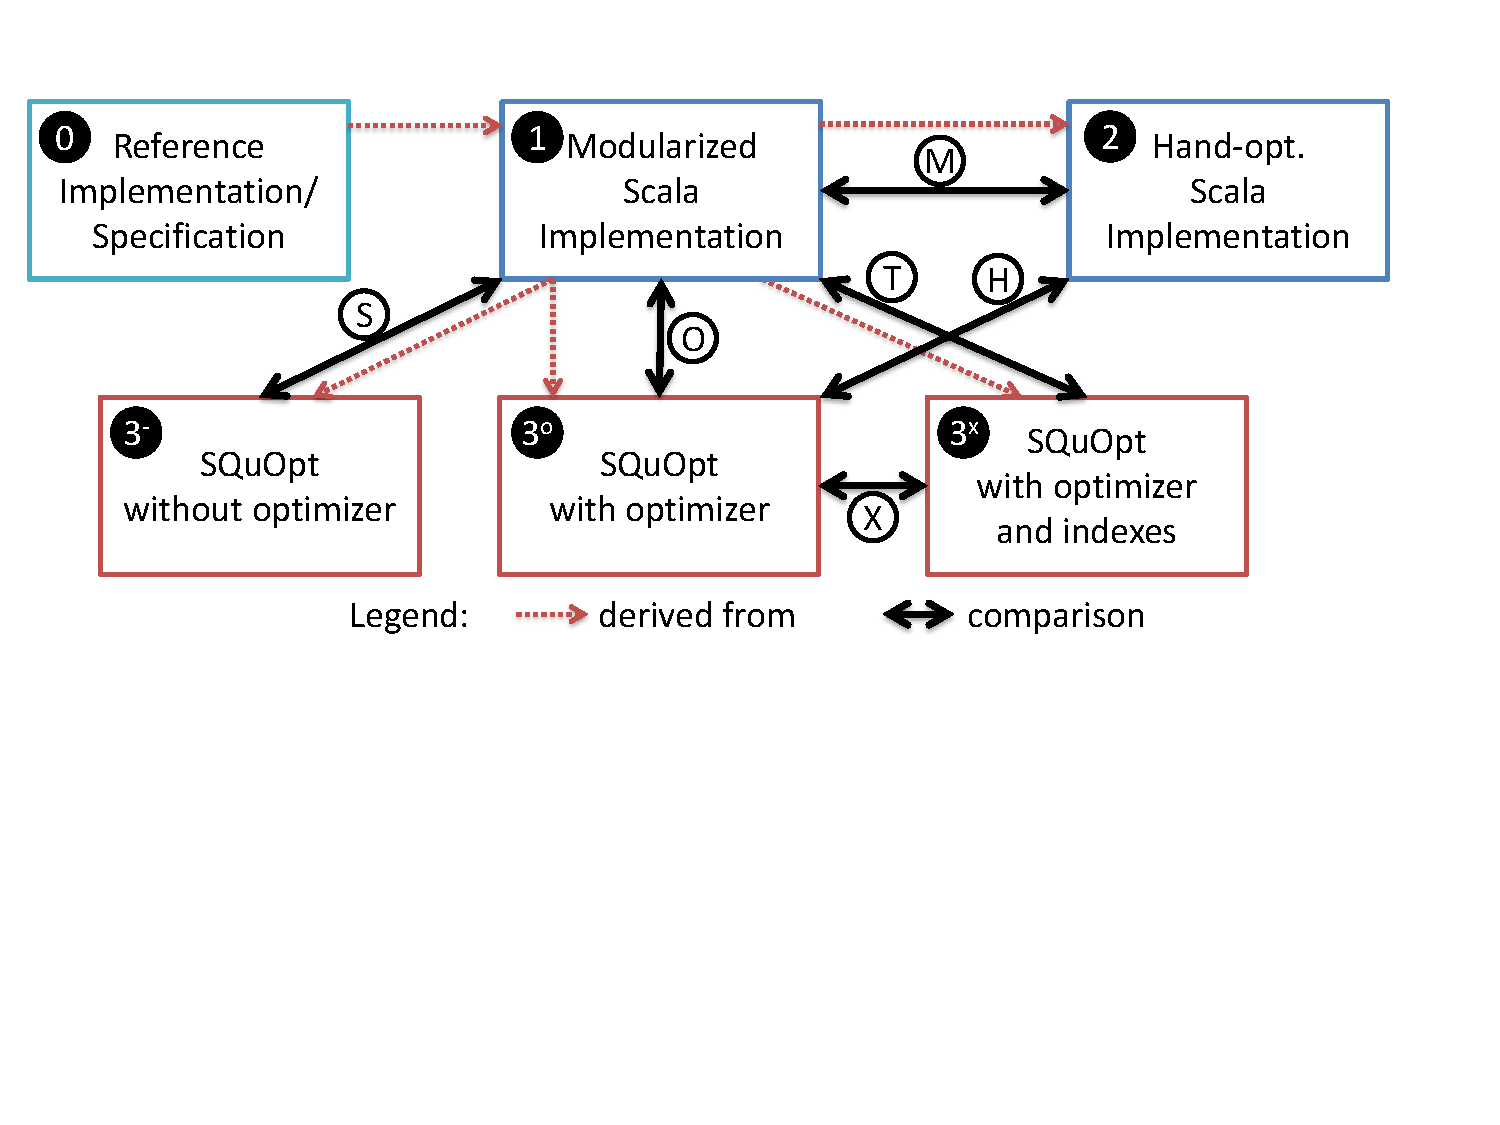
\includegraphics[width=\linewidth]{aosd13/graphs/measurements-overview}
	\caption{Measurement Setup: Overview}
	\label{fig:measurements-overview}
\end{figure}


\section{Experimental Units}




%selecting queries
%\begin{table*}
%\begin{tabular}{ll}\toprule
%Identifier & Description \\ \midrule
%PROTECTED\_FIELD % Findbugs: CI\_CONFUSED\_INHERITANCE
%%	& % Idealized: 4
%	& Class is final but declares protected field \\
%NO\_CLONE % Findbugs: CN\_IDOM
%%	& % Idealized: 9
%	&  Class implements Cloneable but does not define or use clone method \\
%SUPER\_CLONE\_MISSING % Findbugs: CN\_IDIOM\_NO\_SUPER\_CALL
%%	& % Idealized: 11
%	& The clone method does not call super.clone() \\
%NOT\_CLONEABLE % Findbugs: CN\_IMPLEMENTS\_CLONE\_BUT\_NOT\_CLONEABLE
%%	& % Idealized: 5
%	& Class defines clone() but doesn't implement Cloneable\\
%COVARIANT\_COMPARETO % Findbugs CO\_ABSTRACT\_SELF \& CO\_SELF\_NO\_OBJECT
%%	& % Idealized: 7
%	& Covariant compareTo() method defined\\
%GC\_CALL % Findbugs:  DM\_GC
%%	& % Idealized: 12
%	& Explicit garbage collection; extremely dubious except in benchmarking code\\
%RUN\_FINALIZERS\_ON\_EXIT % Findbugs DM\_RUN\_FINALIZERS\_ON\_EXIT
%%	& % Idealized: 12
%	& Method invokes dangerous method runFinalizersOnExit\\
%COVARIANT\_EQUALS %Findbugs: EQ\_ABSTRACT\_SELF
%%	& % Idealized: 4
%	& Abstract class defines covariant equals() method \\
%FINALIZER\_NOT\_PROTECTED % Findbugs: FI_PUBLIC_SHOULD_BE_PROTECTED
%%	& % Idealized: 6
%	& Finalizer should be protected, not public\\
%%NO\_SUITABLE\_CONSTRUCTOR% Findbugs: SE\_NO\_SUITABLE\_CONSTRUCTOR
%%	& % Idealized: 7
%%	& Class is Serializable but its superclass doesn't define a void constructor\\
%UNUSED\_PRIVATE\_FIELD % Findbugs: UUF\_UNUSED\_FIELD
%%	& % Idealized: 23
%	& The value of a private field is not read\\
%DONT\_CATCH\_IMSE  %Findbugs: IMSE\_DONT\_CATCH\_IMSE
%%	& % Idealized: 5
%	& Dubious catching of IllegalMonitorStateException \\\bottomrule
%\end{tabular}
%\nocaptionrule\caption{Implemented Analyses}
%\label{table:implemented-analyses}
%\end{table*}


\newcommand{\captionEvalTable}{%
As in in \cref{sec:implemenationsandspeedups}, (1) denotes the modular Scala
implementation, (2) the hand-optimized Scala one, and ($3^-$), ($3^o$), ($3^x$)
refer to the {\LoS} implementation when run, respectively, without
optimizations, with optimizations, with optimizations and indexing.
Queries marked with the $R$ superscript were selected by random sampling.}
\newcommand{\tablerowsize}{\scriptsize}
\begin{sidewaystable}[ph!]
\centering
\input{\graphPath{EvalTable}}
\nocaptionrule\caption{Performance results. \captionEvalTable}
\label{table:performance}
\end{sidewaystable}



\begin{table}[h]
  \centering
  \footnotesize
\input{\graphPath{EvalSummaryTable}}
\nocaptionrule\caption{Average performance ratios.
This table summarizes all interesting performance ratios across all queries,
using the geometric mean~\citep{Fleming86}.
The meaning of speedups is discussed in \cref{sec:implemenationsandspeedups}.}
\label{table:performanceAvg}
\end{table}

\begin{table}[h!]
\begin{tabular}{p{7cm}r}\toprule
Abstraction & Used \\ \midrule
% calculate class hierarchy & 5 \\
All fields in all class files	& 4\\
All methods in all class files	& 3\\
All method bodies in all class files	& 3\\
All instructions in all method bodies and their bytecode index	& 5\\
Sliding window (size $n$) over all instructions (and their index) &	3\\
\bottomrule
\end{tabular}\\
\nocaptionrule\caption{Description of abstractions removed during hand-optimization and number of queries where the abstraction is used (and optimized away).}
\label{table:implemented-abstractions}
\end{table}

\begin{extraEval}
\begin{table*}[tb]
\centering
\begin{tabular}{l*{3}{r@{}c@{}l}r*{2}{r@{}c@{}l}}\toprule
Name&\multicolumn{3}{c}{Base impl.\ (in ms)}&\multicolumn{3}{c}{Modular impl}&\multicolumn{3}{c}{Optimiz.\ time}&IS&\multicolumn{3}{c}{OS}&\multicolumn{3}{c}{OS-Opt}\\\midrule
\input{\graphPath{table}}
\bottomrule
\end{tabular}
\nocaptionrule\caption{Old performance results table}
\label{table:performanceOld}
\end{table*}
\end{extraEval}


As experimental units, we sampled a set of queries on code structures from FindBugs 2.0~\citep{DBLP:journals/sigplan/HovemeyerP04}. FindBugs is a popular bug-finding tool for Java Bytecode available as open source. To detect instances of bug patterns, it queries a structural in-memory representation of a code base (extracted from bytecode).
Concretely, a single loop traverses each class and invokes all visitors (implemented as listeners) on each element of the class. Many visitors, in turn, perform activities concerning multiple bug detectors which are fused together. An extreme example is that, in FindBugs, query \queryRUNFINALIZERSONEXIT{} is defined in class \code{DumbMethods} together with other 41 bug detectors for distinct types of bugs.
Typically a bug detector is furthermore scattered across the different methods of the visitor, which handle different elements of the class.
We believe this architecture has been chosen to achieve good performance; however, we do not consider such manual fusion of distinct bug detectors together as modular. We selected queries from FindBugs because they represent typical non-trivial queries on in-memory collections and because we believe our framework allows expressing them more modularly.

We sampled queries in two batches. First, we manually selected \manualQueryCount~queries (from approx.\ 400~queries in FindBugs), chosen mainly to evaluate the potential speedups of indexing (queries that primarily looked for declarations of classes, methods, or fields with specific properties, queries that inspect the type hierarchy, and queries that required analyzing methods implementation).
Subsequently, we \emph{randomly} selected a batch of \randomQueryCount~additional queries.
The batch excluded queries that rely on control-/dataflow analyses (i.e., analyzing the effect of bytecode instructions on the stack), due to limitations of the bytecode tookit we use.
In total, we have \queryCount{} queries as listed in \cref{table:performance} (the randomly selected queries are marked with the superscript $R$).




%Omit - this only showcases BAT, not our code. Show our implementation instead.
\begin{figure}[htb]
\centering
%\begin{lstlisting}
%for {
%  cf <- classFiles
%  m @ Method(_, "equals", MethodDescriptor(Seq(cf.thisClass), BooleanType), _) <- cf.methods
%  if m.isAbstract
%} yield (cf, m)
%\end{lstlisting}
%import BATLifting._
\begin{lstlisting}
for {
  classFile <- classFiles.asSquopt
  method <- classFile.methods
  if method.isAbstract && method.name ==# "equals" &&
     method.descriptor.returnType ==# BooleanType
  parameterTypes <- Let(method.descriptor.parameterTypes)
  if parameterTypes.length ==# 1 &&
     parameterTypes(0) ==# classFile.thisClass
} yield (classFile, method)
\end{lstlisting}
\caption{Find covariant \code{equals} methods.}
\label{fig:covariant-equals}
\end{figure}



%reimplementation
We implemented each query three times (see implementations (1)--(3) in \cref{sec:implemenationsandspeedups}) following the specifications given in the FindBugs documentation (0). Instead of using a hierarchy of visitors as the original implementations of the queries in FindBugs, we wrote the queries as for-comprehensions in Scala on an in-memory representation created by the Scala toolkit BAT\@.\footnote{\url{http://github.com/Delors/BAT}}
BAT in particular provides comprehensive support for
writing queries against Java bytecode in an idiomatic way.
We exemplify an analysis in \cref{fig:covariant-equals}: It detects all co-variant \code{equals} methods in a project by iterating over all class files (line 2) and all methods, searching for methods named ``\code{equals}'' that return a boolean value and define a single parameter of the type of the current class.


\smartParagraph{Abstractions}
In the reference implementations (1), we identified several reusable abstractions as shown in \cref{table:implemented-abstractions}.
The reference implementations of all queries except \querySEBADFIELDINNERCLASS{} use exactly one of these abstractions, which encapsulate the main loops of the queries.

\smartParagraph{Indexes}
For executing ($3^x$) (\LoS\ with indexes), we have constructed three indexes to speed up navigation over the queried data of queries 1--\manualQueryCount{}: Indexes for method name, exception handlers, and instruction types. We illustrate the implementation of the method-name index in \cref{fig:indexes}: it produces a collection of all methods and then indexes them using \code{indexBy}; its argument extracts from an entry the key, that is the method name.
We selected which indexes to implement using guidance from \LoS{} itself; during optimizations, \LoS{} reports which indexes it could have applied to the given query. Among those, we tried to select indexes giving a reasonable compromise between construction cost and optimization speedup.
%% If we want to show the raw data, we could use this LaTeX code - but we need updated, and correct, data!
We first measured the construction cost of these indexes:

\begin{center}
\begin{tabular}{l*{1}{r@{}c@{}l}}\toprule
Index&\multicolumn{3}{c}{Elapsed time (ms)}\\\midrule

Method name&$97.99$&$\pm$&$2.94$\\
Exception handlers&$179.29$&$\pm$&$3.21$\\
Instruction type&$4166.49$&$\pm$&$202.85$\\

\bottomrule
\end{tabular}
\end{center}
For our test data, index construction takes less than 200 ms for the first two indexes, which is moderate compared to the time for loading the bytecode in the BAT representation ($\readingClassFilesTime$). Building the instruction index took around 4 seconds, which we consider acceptable since this index maps each type of instruction (e.g.\ \code{INSTANCEOF}) to a collection of all bytecode instructions of that type.
%Valid question: why does the exception-handler index take so much more than the query it optimizes? That's because indexes are interpreted. But it's best not to say it. Also, we already discuss this later convincingly.

%The first index maps any method name to the corresponding methods (together with containing classes), and is used by many different queries. Its implementation is shown in \cref{fig:indexes}: the code shown first produces a collection of all methods and then indexes them using \code{indexBy}; its argument extracts from an entry the key, that is the method name.
%The second index maps any exception type to exception handlers catching them (together with the containing method bodies, methods and class).
%The third index allows to look for occurrences of bytecode instructions of a given type; it maps any type of bytecode instruction (like \code{INVOKESTATIC}, \code{INVOKEVIRTUAL} and so on) to its occurrences.

\begin{figure}
\centering
\begin{lstlisting}
val methodNameIdx: Exp[Map[String, Seq[(ClassFile, Method)]]] = (for {
  classFile <- classFiles.asSquopt
  method <- classFile.methods
} yield (classFile, method)).indexBy(entry => entry._2.name)
\end{lstlisting}
\caption{A simple index definition}
\label{fig:indexes}
\end{figure}



\section{Measurement Setup}
To measure performance, we executed the queries on the preinstalled JDK class library (\texttt{rt.jar}), containing 58M of uncompressed Java bytecode.
We also performed a preliminary evaluation by running queries on the much smaller ScalaTest library, getting comparable results that we hence do not discuss.
Experiments were run on a 8-core Intel Core i7-2600, 3.40 GHz, with 8 GB of RAM, running Scientific Linux release 6.2.
The benchmark code itself is single-threaded, so it uses only one core; however the JVM used also other cores to offload garbage collection.
We used the preinstalled OpenJDK Java version 1.7.0\_05-icedtea and Scala 2.10.0-M7.

We measure steady-state performance as recommended by \citet{Georges07rigorousJavaPerformance}. We invoke the JVM $p = 15$ times;
at the beginning of each JVM invocation, all the bytecode to analyze is loaded in memory and converted into BAT's representation.
In each JVM invocation, we iterate each benchmark until the variations of results becomes low enough. We measure the variations of results through the coefficient of variation (CoV; standard deviation divided by the mean). Thus, we iterate each benchmark until the CoV in the last $k = \kZrememberedSampleLoops$ iterations drops under the threshold $\theta = \thetaZmaxCov$, or until we complete $q = \qZmaxLoops$ iterations.
We report the arithmetic mean of these measurements (and also report the usually low standard deviation on our web page).
%PG: I had p = 3, k = 50, theta = 0.02, q = 1000, but changed the parameters when running more queries.

\section{Results}

\smartParagraph{Correctness} We machine-checked that for each query, all variants in \cref{table:performance} agree.

\smartParagraph{Modularization Overhead}
We first observe that performance suffers significantly when using the abstractions we described in \cref{table:implemented-abstractions}. These abstractions, while natural in the domain and in the setting of a declarative language, are not idiomatic in Java or Scala because, without optimization, they
will obviously lead to bad performance. They are still useful abstractions from the point of view of modularity, though---as indicated by \cref{table:implemented-abstractions}---and as such it would be desirable if one could use them without paying the performance penalty.


\smartParagraph{Scala Implementations vs.\ FindBugs}
Before actually comparing between the different Scala and \LoS\ implementations, we first ensured that the implementations are comparable to the original FindBugs implementation. A direct comparison between the FindBugs reference implementation and any of our implementations is not possible in a rigorous and fair manner. FindBugs bug detectors are not fully modularized, therefore we cannot reasonably isolate the implementation of the selected queries from support code. Furthermore, the architecture of the implementation has many differences that affect performance: among others, FindBugs also uses multithreading. Moreover, while in our case each query loops over all classes, in FindBugs, as discussed above, a single loop considers each class and invokes all visitors (implemented as listeners) on it.

We measured \emph{startup performance}~\citep{Georges07rigorousJavaPerformance}, that is the performance of running the queries only once, to minimize the effect of compiler optimizations.
We setup our \LoS-based analyses to only perform optimization and run the optimized query. To setup FindBugs, we manually disabled all unrelated bug detectors; we also made the modified FindBugs source code available. The result is that the performance of the Scala implementations of the queries ($3^-$) has performance of the same order of magnitude as the original FindBugs queries -- in our tests, the \LoS\ implementation was about twice as fast. However, since the comparison cannot be made fair, we refrained from a more detailed investigation.

% XXX HACK
\smartParagraph{SQuOpt Overhead and Optimization Potential}
We present the results of our benchmarks in \cref{table:performance}.
Column names refer to a few of the definitions described above; for readability, we do not present all the ratios previously introduced for each query, but report the raw data.
In \cref{table:performanceAvg}, we report the geometric mean \cite{Fleming86} of each ratio, computed with the same weight for each query.

%queries are between \maxInterpOver{}x slower and \maxInvInterpOver{}x faster; on average \LoS\ queries are \geoMeanInvInterpOver{}x faster.
%\minInvInterpOver{}x and \maxInvInterpOver{}x---that is, queries are between \minInterpOver{}x and
We see that, in its current implementation, \LoS\ can cause a overhead S
(1/$3^-$) up to \maxInterpOver{}x. On average \LoS\ queries are
\geoMeanInterpOver{}x faster. These differences are due to minor implementation
details of certain collection operators.
For query $18^R$, instead, we have that the the basic \LoS\ implementation is \maxInvInterpOver{}x faster and are investigating the reason; we suspect this might be related to the use of pattern matching in the original query.

As expected, not all queries benefit from optimizations;
out of \queryCount{} queries, optimization affords for \nSpeededUpQueries{} of them significant speedups ranging from a \minOptimSpeedup{} factor to a \maxOptimSpeedup{} factor; \nBigSpeededUpQueries{} queries are faster by a factor of at least \speedupBigThreshold{}.
Only queries \queryMSPKGPROTECT{}, \querySICINNERSHOULDBESTATICANON{} and \queryITAINEFFICIENTTOARRAY{} fail to recover any modularization overhead.

We have analyzed the behavior of a few queries after optimization, to understand why their performance has
(or has not) improved.

Optimization makes query \querySEBADFIELDINNERCLASS{} slower; we believe this is because optimization replaces filtering by lazy filtering, which is usually faster, but not here.
Among queries where indexing succeeds, query \queryGCCALL{} has the least speedup. After optimization, this query uses the instruction-type index to find all occurrences of invocation opcodes (\code{INVOKESTATIC} and \code{INVOKEVIRTUAL}); after this step the query looks, among those invocations, for ones targeting \code{runFinalizersOnExit}. Since invocation opcodes are quite frequent, the used index is not very specific, hence it allows for little speedup (\speedupTGCCALL). However no other index applies to this query; moreover, our framework does not maintain any selectivity statistics on indexes to predict these effects.
Query \queryFIUSELESS{} benefits from indexing without any specific tuning on our part, because it looks for implementations of \code{finalize} with some characteristic, hence the highly selective method-name index applies.
After optimization, query \queryDONTCATCHIMSE{} becomes simply an index lookup on the index for exception handlers, looking for handlers of \code{IllegalMonitorStateException}; it is thus not surprising that its speedup is thus extremely high (\maxOptimSpeedup{}). This speedup relies on an index which is specific for this kind of query, and building this index is slower than executing the unoptimized query. On the other hand, building this index is entirely appropriate in a situation where similar queries are common enough. Similar considerations apply to usage of indexing in general, similarly to what happens in databases.

\smartParagraph{Optimization Overhead}
The current implementation of the optimizer is not yet optimized for speed (of the optimization algorithm). For instance, expression trees are traversed and rebuilt completely once for each transformation.
However, the optimization overhead is usually not excessive and
is $\avgOptimTime \pm \stdDevOptimTime$ ms, varying between \minOptimTime{} ms and \maxOptimTime{} ms (mostly depending on the query size).

\smartParagraph{Limitations}
Although many speedups are encouraging, our optimizer is currently a proof-of-concept and we experienced some limitations:
\begin{itemize}
\item In a few cases hand-optimized queries are still faster than what the optimizer can produce. We believe these problems could be addressed by adding further optimizations.
\item Our implementation of indexing is currently limited to immutable collections. For mutable collections, indexes must be maintained incrementally.
Since indexes are defined as special queries in {\LoS},  incremental index maintenance becomes an instance of incremental maintenance of query results, that is, of incremental view maintenance. We plan to support incremental view maintenance as part of future work; however,
indexing in the current form is already useful, as illustrated by our experimental results.
\end{itemize}

\smartParagraph{Threats to Validity}
With rigorous performance measurements and the chosen setup, our study was setup to maximize internal and construct validity. Although we did not involve an external domain expert and we did not compare the results of our queries with the ones from FindBugs (except while developing the queries), we believe that the queries adequately represent the modularity and performance characteristics of FindBugs and {\LoS}. However, since we selected only queries from a single project, external validity is limited.
While we cannot generalize our results beyond FindBugs yet, we believe that the FindBugs queries are representative for complex in-memory queries performed by applications.


\smartParagraph{Summary}
We demonstrated on our real-world queries that relying on declarative abstractions in collection queries often causes a significant slowdown. As we have seen, using \LoS\ without optimization, or when no optimizations are possible, usually provides performance comparable to using standard Scala; however, \LoS\ optimizations can in most cases remove the slowdown due to declarative abstractions. Furthermore, relying on indexing allows to achieve even greater speedups while still using a declarative programming style.
Some implementation limitations restrict the effectiveness of our optimizer, but since this is a preliminary implementation, we believe our evaluation shows the great potential of optimizing queries to in-memory collections.


% vim: set tw=0:


\section{Related Work}
\label{sec:relwork}
This paper builds on prior work on language-integrated queries, query optimization, techniques for DSL embedding, and other works on code querying.

\smartParagraph{Language-Integrated Queries}
Microsoft's Language-Integrated Query technology (\LINQ)~\citep{Meijer:2006:LRO:1142473.1142552,Bierman:2007:LTF:1297027.1297063} is similar to our work in that it also
reifies queries on collections to enable analysis and optimization. Such queries can be executed against a variety of backends (such as SQL databases or in-memory objects), and adding new back-ends is supported. Its implementation uses \emph{expression trees}, a compiler-supported
implicit conversion between expressions and their reification as a syntax tree. There are various major differences, though.
First, the support for expression trees is hard-coded into the compiler. This means that the techniques are not applicable in languages 
that do not explicitly support expression trees. More importantly, the way expression trees are created in \LINQ\ is generic and fixed.
For instance, it is not possible to create different tree nodes for method calls that are relevant to an analysis (such as the \code{map} method) than for method calls that are irrelevant for the analysis (such as the \code{toString} method). For this reason, expression trees in \LINQ\ 
cannot be customized to the task at hand and contain too much low-level information. It is well-known that this makes it quite hard to
implement programs operating on expression trees~\citep{Eini11Pain}. 

\LINQ\ queries can also not easily be decomposed and modularized. For instance, consider the task of refactoring the filter in the query {\tt from x in y where x.z == 1 select x}
into a function. Defining this function as {\tt bool comp(int v) \{ return v == 1; \}} would destroy the possibility of analyzing the filter for optimization, since
the resulting expression tree would only contain a reference to an opaque function. The function could be declared as returning an expression tree instead, but then
this function could not be used in the original query anymore, since the compiler expects an expression of type {\tt bool} and not an expression tree of type {\tt bool}.
It could only be integrated if the expression tree of the original query is created by hand, without using the built-in support for expression trees.

% Klaus: since we do not talk much about the embedding technique we should not talk about type safety here
%Expression trees in \LINQ\ also provide little type safety. While they appear to be typed superficially (quoting an expression of type \code{T} yields 
%an expression tree of type \code{Expression<T>}) they are untyped internally. For instance, when one decomposes a node into its components,
%the components are untyped. 
% Klaus: let's not distract by talking superficially about Haskell
% This is similar to deep embedding of expressions in Haskell, which typically use a phantom type wrapper around untyped expressions.

%In contrast, expression trees in our approach are typed and simple transformations can be statically checked to be type-preserving. More complex optimizations require however type casts and rely on erasure of type parameters at run time, as we will discuss in detail later on.

Although queries against in-memory collections could theoretically also be optimized in \LINQ, the standard implementation, {\LINQ}2Objects, performs no optimizations. 

A few optimized embedded DSLs allow executing queries or computations on distributed clusters.
DryadLINQ~\citep{Yu08}, based on \LINQ, optimizes queries for distributed
execution. It inherits \LINQ's limitations and thus does not support decomposing queries in different modules.
Modularizing queries is supported instead by FlumeJava~\citep{Chambers10},
another library (in Java) for distributed query execution.
However, FlumeJava cannot express many optimizations because its representation
of expressions is more
limited; also, its query language is more cumbersome. Both problems are rooted
in Java's limited support for embedded DSLs.
Other embedded DSLs support parallel platforms such as GPUs or many-core CPUs,
such as Delite~\citep{Rompf13}.

\citet{Willis06JQL,Willis08} add first-class queries to Java through a source-to-source translator and implement a few selected optimizations, including join order optimization and incremental maintenance of query results.
They investigate how well their techniques apply to Java programs, and they suggest that programmers use manual optimizations to avoid expensive constructs like nested loops. While the goal of these works is similar to ours, their implementation as an external source-to-source-translator makes
the adoption, extensibility, and composability of their technique difficult%
%~\citep{ErdwegGR12}
.
%KO: not sure whether the reference here helps
%PG: Remove it if we have space limits.

There have been many approaches for a closer integration of SQL queries into programs, such as
HaskellDB~\citep{Leijen99DSEC} (which also inspired \LINQ), or Ferry~\citep{Grust:2009:FDP:1559845.1559982} 
(which moves part of a program execution to a database). In Scala, there are also
APIs which integrate SQL queries more closely such as
Slick.\footnote{\url{http://slick.typesafe.com/}} Its frontend allows to define
and combine type-safe queries, similarly to ours (also in the way it is
implemented).
However, the language for defining queries maps to SQL, so it does not support nesting collections
in other collections (a feature which simplified our example in
Sec.~\ref{sec:motivation}), nor distinguishes statically between different kinds of
collections, such as \code{Set} or \code{Seq}.
Based on Ferry, ScalaQL~\citep{JOT:issue_2010_07/article3} extends Scala with a compiler-plugin to integrate a query language on top of a relational database. The work by \citet{Spiewak09scalaql:language-integrated} is
 unrelated to~\citep{JOT:issue_2010_07/article3} but also called ScalaQL\@. It is similar to our approach in that it also 
proposes to reify queries based on for-comprehensions, but it is not clear from the paper how the reification 
works.\footnote{We contacted the authors; they were not willing to provide more details or the sources of their approach.}


\smartParagraph{Query Optimization}
Query optimization on relational data is a long-standing issue in the database community, but there
are also many works on query optimization on objects~\citep{Fegaras00,Grust99PhD}.
Compared to these works, we have only implemented a few simple query optimizations, so there is potential
for further improvement of our work by incorporating more advanced optimizations.

%CQEngine (\url{http://code.google.com/p/cqengine/}) does not support path
%indexes. It support standing queries - but those are just incrementally
%maintained queries, as far as it seems. But the system is quite cool.
%---

% That's not strictly true, and is not the point. The point is a consequence: in a monoid comprehension for a given monoid, a generator cannot range over a monoid which is weaker wrt.\ idempotence or commutativity.

%For instance, while the formal analogous of folds in their calculus is a monoid homomorphism, computing the size of a Set can be expressed through a fold but not through a monoid homomorphism, since it is a fold from an idempotent to a non-idempotent monoid.

% Klaus: I think this is not that relevant for ICSE
%\citet{Henglein10} present an embedding of the relational algebra in Haskell.
%Queries are not reified in their approach, but due to a particularly sophisticated
%representation of multisets it is possible to execute some queries containing
%cross-products using faster equi-joins.


\smartParagraph{Scala and DSL Embedding}
\label{sec:rwdsl}
Technically, our implementation of \LoS\ is a deep embedding of a part of the Scala collections API~\citep{odersky2009fighting}.
Deep embeddings were pionereed by \citet{Leijen99DSEC} and \citet{elliott03compiling}. The technical
details of the embedding are not the main topic of this paper; we are using some of the 
Scala techniques presented by \citet{rompf2010lightweight} for using implicits and for
adding infix operators to a type. Similar to \citet{rompf2010lightweight}, we also 
use the Scala compiler on-the-fly. A plausible alternative backend for \LoS\ would
have been to use Delite~\citep{Rompf11BBlocks}, a framework for
building highly efficient DSLs in Scala.
Using this framework, in concurrent work, \citet{Rompf13} also optimize
collection queries; while their work allows for imperative programs, they do
not support embedding arbitrary libraries in an automated way. On the other
hand, they can reuse support for automatic parallelization and multiple platforms present in Delite.
\citet{Ackermann12} present Jet, which also optimizes collection queries but
targets MapReduce-style computations in a distributed environment.
Moreover, both works do not apply typical database optimizations such as
indexing or filter hoisting.


We regard the Scala collections API~\citep{odersky2009fighting} as a shallowly embedded query DSL\@. Query operators immediately perform collection operations when called, so that it is not possible to optimize queries before execution. In addition to these eager query operators, the Scala collections API also provides \emph{views} to create lazy collections.
Views are somewhat similar to {\LoS} in that they reify query operators as data structures and interpret them later.
However, views are not used for automatic query optimization, but for explicitly changing the evaluation order of collection processing. Unfortunately, views are not suited as a basis for the implementation of {\LoS} because they only reify the outermost pipeline of collection operators, whereas nested collection operators as well as other Scala code in queries, such as filter predicates or \code{map} and \code{flatMap} arguments, are only shallowly embedded.
Deep embedding of the whole query is necessary for many optimizations, as discussed in Sec.~\ref{sec:solution}.

\smartParagraph{Code Querying}
In our evaluation we explore the usage of \LoS\ to express queries on code and re-implement a subset of the FindBugs~\citep{DBLP:journals/sigplan/HovemeyerP04} analyses. There are various other specialized code query languages such as 
CodeQuest~\citep{Hajiyev06CodeQuest} or D-CUBED~\citep{Wegrzynowicz:2009:GBU:1639950.1640032}. 
Since these are special-purpose query languages that are not embedded into a host language, they are not directly comparable to our approach.



\section{Future Work}
As part of future work we plan to add support for \emph{incremental view
maintenance}~\citep{GlucheGrust97Incr} to \LoS. This would allow, for instance,
to update incrementally both indexes and query results.

To make our DSL more convenient to use, it would be useful to use the
virtualized pattern matcher of Scala 2.10, when it will be more robust, to add
support for pattern matching in our virtualized queries.

Finally, while our optimizations are type-safe, as they rewrite an expression
tree to another of the same type, currently the Scala
type-checker cannot verify this statically, because of its limited support for
GADTs.
Solving this problem conveniently would allow checking statically that
transformations are safe and make developing them easier.

\section{Conclusions}

We have illustrated the tradeoff between performance and modularity for queries on in-memory collections. We have shown that it is possible to design a deep embedding of a version of the collections API which reifies queries and can optimize them at runtime.
Writing queries using this framework is, except minor syntactic details, the same as writing queries using the collection library, hence the adoption barrier to using our optimizer is low. 

Our evaluation shows that using abstractions in queries introduces a significant
performance overhead with native Scala code, while \LoS{}, in most cases, makes
the overhead much more tolerable or removes it completely. Optimizations are not
sufficient on some queries, but since our optimizer is a proof-of-concept with
many opportunities for improvement, we believe a more elaborate version will
achieve even better performance and reduce these limitations.


%\section*{Acknowledgements}
\smartParagraph{Acknowledgements}
The authors thank Sebastian Erdweg for helpful discussions on
this project, Katharina Haselhorst for help
implementing the code generator, and the anonymous reviewers, Jacques Carette and Karl Klose
for their helpful comments on this paper.
This work is supported in part by the European Research Council, grant \#203099 ``ScalPL''.



\part{Incrementalization}
\label{part:incr}
\chapter{Introduction to static differentiation}
% Emacs, this is -*- latex -*-!

\section{Introduction}
\label{sec:intro}

Incremental computation has a long-standing history in computer
science~\citep{Ramalingam93}. Often, a program needs to update its
output efficiently to reflect input
changes~\citep{Salvaneschi13reactive}. Instead of rerunning such a
program from scratch on its updated input, incremental
computation research looks for alternatives that are cheaper in a common scenario:
namely, when the input change is much smaller than the input itself.

For instance, consider the $\Program$ program, which calculates
the sum of all numbers in collections $\Xs$, $\Ys$.
\begin{align*}
\Program & = \ProgramBody\\
\Output & = \Program~\Set{1,1}~\Set{2,3,4}=11
\end{align*}
With $\Set{\ldots}$ we represent a multiset or \emph{bag}, that is an unordered collection (like a set)
where elements are allowed to appear more than once (unlike a set).
Now assume that the input $\Xs$ changes from $\Set{1,1}$ to
$\Set{1}$, and $\Ys$ changes from $\Set{2,3,4}$ to $\Set{2,3,4,5}$.
Instead of recomputing $\Output$ from scratch, we could also compute it incrementally. If we have a
representation for the changes to the inputs (say,
$\DXs = \Set{\Keyword{remove} \; 1}$,
$\DYs = \Set{\Keyword{add} \; 5}$), we can compute the new
result through a function $\Derivative$ that takes the old inputs
$\Xs = \Set{1,1}$, $\Ys=\Set{2,3,4}$ and the changes $\DXs$,
$\DYs$ to produce the output change.
In this case, it would compute the change
$\Derivative~\Xs~\DXs~\Ys~\DYs = \Keyword{plus} \; 4$,
which can then be used to update the original output $11$
%
to yield the updated result $15$. We call $\Derivative$ the \emph{derivative} of $\Program$.
It is a function in the
same language as $\Program$, accepting and producing changes, which
are simple first-class values of this language.
%
If we increase the size of the original inputs $\Xs$ and $\Ys$, the time
complexity of $\Program~\Xs~\Ys$ increases linearly, while the time complexity
of $\Derivative~\Xs~\DXs~\Ys~\DYs$ only depends on the size of $\DXs$ and $\DYs$,
which is smaller both in our example and in general.

To support automatic incrementalization, in this chapter we introduce the \ILC\
(incrementalizing $\Gl$-calculi) framework. We define
an automatic program transformation $\DERIVE$
that \emph{differentiates} programs, that is, computes their
derivatives; $\DERIVE$ guarantees that
\begin{equation}
  \label{eq:correctness}
\App{f}{\Apply*{\D a}{a}}
\cong
\Apply{\App*{\App{\Derive{f}}{a}}{\D a}}{\App*{f}{a}}.
\end{equation}
where
$\cong$ is denotational equality,
$\D a$ is a change on $a$ and $\Apply{\D a}{a}$ denotes $a$
updated with change $\D a$, that is, the updated input of $f$.
Hence, we can optimize programs by replacing the left-hand side,
which recomputes the output from scratch, with the right-hand
side, which computes the output incrementally using derivatives.
% KO: I think this forward references confuses more than it helps.
%Our approach relates to \emph{finite differencing} but has a more
%general theory and support for first-class functions (see
%\cref{sec:finite-diff}).

\ILC\ is based on a simply-typed $\Gl$-calculus
parameterized by \emph{plugins}. A plugin
defines
%
(a) base types and primitive operations, and
%
(b) a change representation for each base type, and an
incremental version for each primitive. In other words, the plugin
specifies the primitives and their respective derivatives, and
\ILC\ can glue together these simple derivatives in such a way
that derivatives for arbitrary simply-typed $\Gl$-calculus expressions
using these primitives can be computed. Both our implementation and our correctness proof 
is parametric in the plugins, hence it is easy to support (and prove correct)
new plugins.

This chapter makes the following contributions:
\begin{itemize}
\item We present a novel mathematical theory of changes and derivatives, which is more
  general than other work in the field because changes are
  first-class entities, they are distinct from base values and
  they are defined also for functions (\cref{sec:1st-order-changes}).
  %KO: I think the next sentence cannot be understood at this point.
  %We introduce changes for complex types, defined compositionally.
%
\item We present the first approach to incremental computation for
pure $\lambda$-calculi by a source-to-source transformation, $\DERIVE$, that requires no run-time
support. The transformation produces an incremental program in the same language;
all optimization techniques for the original program are
applicable to the incremental program as well.
%KO: commented this out. I think the purity is not important enough
%to deserve another sentence here, since we only vaguely hint
%at "further research".
%Since our incremental programs use no impure features, they are
%especially amenable to further optimizations, making this approach
%very suitable for further research.
%
% KO: Let's have one bullet point per section. Also, a conjecture
% sounds like a rather weak contribution
%\item We argue that incrementalization is efficient on
%  \emph{self-maintainable programs}, and discuss how further research on
%  static or dynamic memoization can speed up a larger class of programs (\cref{sec:performance-cons}).
%  \pg{This contribution references text which is now commented
%    out. I believe the text should be brought back in.}
%
We prove that our incrementalizing transformation $\DERIVE$
is correct~(\cref{eq:correctness})
by a machine-checked formalization in Agda~\citep{agda-head}.
The proof gives insight into the definition of $\DERIVE$: we
first construct the derivative $\EvalInc{-}$ of the denotational
semantics of a simply-typed $\lambda$-calculus term, that is, its
\emph{change semantics}.
%
Then, we show that $\DERIVE$ is produced by erasing
$\EvalInc{-}$ to a simply-typed program (\cref{sec:correctness}).

\item While we focus mainly on the theory of changes
and derivatives, we also perform a performance case study.
We implement the derivation transformation in Scala,
with a plug-in architecture that can be extended with new base
types and primitives. We define a plugin with support for
different collection types and use the plugin to 
incrementalize a variant of the MapReduce programming model~\citep{Lammel07}.
  Benchmarks show that on this program,
  incrementalization can reduce asymptotic complexity and can turn $O(n)$
  performance into $O(1)$, improving running time by over 4
  orders of magnitude on realistic inputs (\cref{sec:applying}).

\end{itemize}

% KO: We said all that is in this paragraph before.
% Our formalization is generic in the set of base types and the set
% of primitives that operate on these base types. That is, we
% present only the core of the formalization that deals with
% function types, lambda abstraction, application and variable
% references. Base types and primitives on base types have to be
% added as plugins. The interface between the core formalization
% and the plugins is formalized as well. It consists of the sets,
% operations, and lemmas that a plugin has to provide in order to
% fit into the core formalization. We hope that the generic
% formalization allows us and other researchers to experiment with
% different choices of base types, and different incrementalization
% strategies for these base types.

%We mechanized the formalization, including the separation between
%core and plugins, in the dependently typed programming language
%Agda~\cite{agda-head}.
Our Agda formalization, Scala implementation and benchmark
results are available at the URL
\url{http://inc-lc.github.io/}.
All lemmas and theorems presented
in this chapter have been proven in Agda.
In the chapter, we present an overview of
the formalization in more human-readable form, glossing over some
technical details.

% KO: Old stuff which contains snippets to be integrated in other sections, in 
% particular Related Work.


\chapter{A theory of changes}
% Include either-or, one includes the other.
%\input{change-theory-reconstruct}
% Emacs, this is -*- latex -*-!
%\section{Changes as First-Class Values}
\section{A theory of changes}
\label{sec:1st-order-changes}

This section introduces a formal concept of changes; this
concept was already used informally in \cref{eq:correctness} and is central
to our approach. We first define change structures formally, then construct 
change structures for functions between change structures,
and conclude with a theorem that relates function changes to derivatives. 

\subsection{Change structures}\label{ssec:change-structures}
Consider a set of values, for instance the set of natural numbers
$\mathbb{N}$. A change $\D v$ for $v \in \mathbb{N}$ should
describe the difference between $v$ and another natural $\New{v}
\in \mathbb{N}$. We do not define changes directly, but we
specify operations which must be defined on them. They are:
\begin{itemize}
\item We can \emph{update} a base value $v$ with a
  change $\D v$ to obtain an updated or \emph{new} value
  $\New{v}$. We write $\New{v} = \Apply{\D v}{v}$.
\item We can compute a change between two arbitrary
  values $\Old{v}$ and $\New{v}$ of the set we are considering.
  We write $\D v = \Diff{\New{v}}{\Old{v}}$.
\end{itemize}

For naturals, it is usual to describe changes using standard
subtraction and addition. That is, for naturals we can define
$\Apply{\D v}{v} = v + \D v$ and $\Diff{\New{v}}{\Old{v}} =
\New{v} - \Old{v}$. To ensure that $\APPLY$ and $\DIFF$ are
always defined, we need to define the set of changes carefully.
$\mathbb{N}$ is too small, because subtraction does not always
produce a natural; the set of integers $\mathbb{Z}$ is instead
too big, since adding a natural and an integer does not always
produce a natural. In fact, we cannot use the same set of all
changes for all naturals. Hence we must adjust the requirements:
for each base value $v$ we introduce a set $\Change{v}$ of
changes for $v$, and require $\Diff{\New{v}}{\Old{v}}$ to produce
values in $\Change{\Old{v}}$, and $\Apply{\D v}{v}$ to be defined
for $\D v$ in $\Change{v}$. For natural $v$, we set $\Change{v} =
\left\{\D v \mid v + \D v \geq 0 \right\}$; $\DIFF$ and $\APPLY$ are
then always defined.

\begin{oldSec}

\ldots, we could use \emph{functional
changes}, that is by defining changes to be functions from the
old value to the new value:
\begin{align*}
\Change{\Gt} & = \Gt \r \Gt, \\
\Apply{\D v}{\Old{v}} & = \App{\D v}{\Old{v}},\\
\Diff{\New{v}}{\Old{v}} & = \Lam{x}{\New{v}}.
\end{align*}
However,
this definition does not allow derivatives to analyze changes to
be more efficient than recomputation. To understand why, let us
consider the following example.

Let $\Old{v} = \{1, 2, \ldots, n\}$ be a bag (or multiset) of
integers, let $f$ be a function from bags to integers summing the
elements of its argument, and let $\Old{s} = \App{f}{\Old{v}}$.

Later during program execution, assume we add $n + 1$ to
$\Old{v}$ and need to update $\Old{s}$. Hence,
 $\New{v} = \{1, 2, \ldots, n, n + 1\}$, $\D v$ represent the change of $v$,
and we need to compute the result of $\New{s} = \App{f}{\New{v}}$.
%
Thanks to \cref{eq:correctness}, we can guarantee that
$\New{s} = \Apply{\App{\App{\Derive{f}}{\Old{v}}}{\D
    v}}{\Old{v}}$.

Now, if $\Derive{f}$ would know that $\D v$ only added $n + 1$ to
the bag, it could produce in $O(1)$ a change $\D s$ such that
$\Apply{\D s}{s} = n + 1 + s$. But if $\D v$ is simply a function
such that $\App{\D v}{\Old{v}} = \New{v}$, we have no way of
inspecting its intension, since in $\lambda$-calculus functions
are opaque. Instead, the difference between two bags can be
described as another bag, and $\APPLY$ for bags can be defined as
bag merge.%
\footnote{Negative multiplicities are required to represent
  removals, as we discuss in Sec.~\ref{sec:plugins}.} Similarly,
we can describe the difference between two numbers $x$ and $y$ as
their arithmetical difference $x-y$. In this case, the change
application operator $\APPLY$ would be the normal addition
operator $+$. With these definitions, thanks to the structure of
$+$, $\App{\App{\Derive{f}}{\Old{v}}}{\D v}$ can produce its
result without even using $\Old{v}$, in time $O(|\D v|)$ (we
explain later how to compute $\Derive{f}$ automatically).

For now, we simply note that we cannot fix $\Change{\Gt} = \Gt \r
\Gt$. We need a more flexible encoding of changes, which allows
inspecting their structure; moreover, this structure needs to
allow writing efficient derivatives, in particular efficient
derivatives for the primitives acting on $\Gt$.

Hence, to make our general framework
independent of such domain- and application-specific
considerations, we simply require language plugins to define not
only base types and primitives for them, but also $\Change{\tau}$
whenever $\tau$ is a base type, and operators $\APPLY_\tau$ and
$\DIFF_\tau$.
Using $\APPLY$, we can recover a function $\Gt\r\Gt$
from any $\D x$ of type $\Change{\Gt}$; it is $\Lam*x{\Apply{\D
x}{x}}$.
\end{oldSec}

\pg{We never say why we use ``structure''. On second thought,
  this might be OK since we have little space.}
The following definition sums up the discussion so far:

\pg{Consider less heavyweight phrasing, such as: ``To each $v \in V$
  we associate a set of changes $\Change{v}$. But do this consistently.}
\begin{definition}[Change structures]
  \label{def:change-struct}
  A tuple $\ChangeStruct{V} = (V, \CHANGE,
  \UPDATE,
  \DIFF)$ is a \emph{change structure} (for $V$) if:

  \begin{subdefinition}
  \item $V$ is a set, called the \emph{base set}.
  \item Given $v \in V$, $\Change{v}$ is a set, called the \emph{change set}.
  \item Given $v \in V$ and $\D v \in \Change{v}$, $\Apply{\D v}{v} \in V$.
    \label{def:update}
  \item Given $u, v \in V$, $\Diff{u}{v} \in \Change{v}$.
    \label{def:diff}
  \item Given $u, v \in V$, $\Apply{\Diff*{u}{v}}{v}$ equals $u$.
    \qed
    \label{def:update-diff}
  \end{subdefinition}
\end{definition}

One might expect a further assumption that
$\Diff{\Apply*{\D v}{v}}{v} = \D v$. While it does hold
for the change structure of $\mathbb{N}$, it is not needed in general.
This means that multiple changes can represent the difference between
the same two base values. Throughout our theory, we only discuss equality of
base values, not of changes.

\paragraph{Notation}
We overload operators $\CHANGE$, $\DIFF$ and $\UPDATE$ to refer
to the corresponding operations of different change structures;
we will subscript these symbols when needed to prevent ambiguity.
For any $\ChangeStruct{S}$, we write $S$ for its first component,
as above. We make $\UPDATE$ left-associative, that is,
$\Update{\Update{v}{dv_1}}{dv_2}$ means $\Update{\Update*{v}{dv_1}}{dv_2}$.
We assign precedence to function application over
$\UPDATE$ and $\DIFF$, that is, $\Update{\App{f}{a}}{\App{\App{g}{a}}{\D a}}$ means
$\Update{\App*{f}{a}}{\App*{\App{g}{a}}{\D a}}$.

\begin{examples}
We demonstrate a change structure on \emph{bags with signed
multiplicities}~\citep{Koch10IQE}.
These are
unordered collections where each element can appear an integer
number of times. 
\begin{enumerate}[(a)]
\item
Let $S$ be any set.
The base set $V=\Bag S$ is the set of bags of elements of $S$ with signed
multiplicities. The bag $\Set{1,1,\bar2}$ contains two positive
occurrences of $1$ and a negative occurrence of $2$.

\item For each bag $v\in V$, set the change set $\Change v = V$.
Every bag can be a change to any other bag. The bag
$\Set{1,1,\bar5}$ represents two insertions of $1$ and one
deletion of $5$.

\item The update operator is bag merge: $\UPDATE=\MERGE$. The
merge of two bags is the element-wise sum of multiplicities:
\[
\Merge{\Set{\bar1,2}}{\Set{1,1,\bar5}}=\Set{1,2,\bar5}.
\]

\item Let $\NEGATE$ be the negation of multiplicities:
\[
\Negate{\Set{1,1,\bar5}}=\Set{\bar1,\bar1,5}.
\]
To compute the
difference of two bags, compute the merge with a negated bag:
\[
\Diff{u}{v}=\Merge{u}{\Negate*{v}}.
\]

\item Given the above definition of $\UPDATE$ and $\DIFF$, it is
not hard to show that $\Apply{\Diff*{u}{v}}{v}$ for all bags
$u,v\in V$.
\end{enumerate}
The change structure we just described is written succinctly
\begin{alignat*}3
\ChangeStruct{\Bag S} = (
&\Bag S,
&&\Lam*{v} {\Bag S},
\\
&\MERGE,
&&\Lam*{x\; y}{\Merge{x}{\Negate*{y}}}).
\end{alignat*}

This change structure is an instance of a general construction:
we can build a change structure from an arbitrary \emph{abelian group}.
An abelian group is a tuple $(G, \boxplus,
\boxminus, e)$, where $\boxplus$ is a commutative
and associative binary operation, $e$ is its identity
element, and $\boxminus$ produces inverses of elements $g$
of $G$, such that $(\boxminus g) \boxplus g = g \boxplus
(\boxminus g) = e$. For instance, integers,
unlike naturals, form the abelian group $(\mathbb{Z}, +, -, 0)$
(where $-$ represents the unary minus). Each abelian group
$(G, \boxplus, \boxminus, e)$ induces a change structure,
namely $\left(G, \Lam{g}{G}, \boxplus, \Lam{g\; h}{g
    \boxplus (\boxminus h)}\right)$, where the change set
for any $g \in G$ is the whole $G$. Change structures
are more general, though, as the example with natural numbers illustrates.
%
If $\Empty$ represents the empty bag, then $(\Bag{S}, \MERGE,
\NEGATE, \Empty)$ is an abelian group, which induces the
change structure we have just seen.

The abelian group on integers induces also a change structure on
integers, namely $\ChangeStruct{\mathbb{Z}} = (\mathbb{Z},
\Lam*{v} {\mathbb{Z}}, +, -)$.
\end{examples}

\paragraph{Nil changes and derivatives}
A particularly important change is the \emph{nil change} of a value:
\begin{definition}[Nil change]
  \label{def:nil-change}
  Given a change structure $\ChangeStruct{V}$ and a value $v \in V$, the change
  $\Diff{v}{v}$ is the nil change for $v$.
  \[
    \Nil{v} = \Diff{v}{v} \qed
  \]
\end{definition}
The nil change for a value does indeed not change it.
\begin{lemma}[Behavior of $\NIL$]
  \label{thm:update-nil}
  Given a change structure $\ChangeStruct{V}$ and a value $v \in V$,
  $\Apply{\Nil{v}}{v} = v$.
\end{lemma}

\begin{optionalproof}
Follows from \cref{def:update-diff,def:nil-change}.
\end{optionalproof}

\pg{Maybe should move this before nil changes?}
After defining change structures, we can restate the definition of derivatives from \cref{eq:correctness}.

\begin{definition}[Derivatives]
  \label{def:derivatives}
  Given change structures $\ChangeStruct{A}$ and $\ChangeStruct{B}$ and a function $f \in A \to
  B$ on the change sets of these change structures, we call a binary function $f'$ the \emph{derivative} of $f$ if
  for all values $a \in A$ and corresponding changes $\D a \in
  \Change[A]{a}$,
  \[\App{f}{\Apply*{\D a}{a}} = \Apply{\App{\App{f'}{a}}{\D a}}{\App{f}{a}}\text{.}\qed\]
\end{definition}

Applying a derivative to a value and its nil change gives a nil
change.%
\footnote{Post-print note: There's a small technical mistake in
  the following lemma. See \cref{sec:change-eq} for a corrected
  statement.}
%
\begin{lemma}[Behavior of derivatives on $\NIL$]
  \label{thm:deriv-nil}
  Given change structures $\ChangeStruct{A}$ and
  $\ChangeStruct{B}$, a function $f \in A \to B$, an element $a$
  of $A$, and the derivative $f'$ of $f$, we have
  $\App{\App{f'}{a}}{\Nil{a}} = \Nil{\App* f a}$.
\end{lemma}

\begin{examples}
Let $\Term{f}:\Fun{\Bag S}{\Bag S}$ be the constant function mapping
everything to the empty bag. Its derivative
$\Term{f'}:\Fun{\Bag S}{\Fun{\Bag S}{\Bag S}}$ has to ignore its two
arguments and produce the empty bag in all cases.

Let $\Term{id}:\Fun{\Bag S}{\Bag S}$ be the identity function between
bags. Its derivative $\Term{id'}$ is defined by
$\Term{id'}~v~\D v = \D v$.
\end{examples}

% Emacs, this is -*- latex -*-!
\subsection{Function changes}
\label{sec:function-change}

% moved here to avoid annoying out-of-order figures.
% Emacs, this is -*- latex -*-!
\begin{figure*}
\begin{tabular}{>{$}r<{$}@{$\;::=\;$}>{$}c<{$}@{$\;$}>{$}l<{$}@{\quad}>{(}l<{)}}
\Gi      & \rlap{\ldots} &                       & base types\\
\Gs, \Gt & \Gi           & \mid \Fun{\Gt}{\Gt}   & types\\
\GG      & \EmptyContext & \mid \Extend{x}{\tau} & typing contexts\\
c        & \rlap{\ldots} &                       & constants\\
s, t     & c             & \mid \Lam{x}{t}
                           \mid \App{t}{t}
                           \mid x                & terms
\end{tabular}
\caption{Our base calculus: Syntax}
\label{fig:syntax}
\end{figure*}

\begin{figure*}
\begin{typing}
\noindent
\Rule[Const]
  {\ldots}
  {\Typing[]{c}{\tau}}

\Axiom[Lookup]
  {\Typing[\Append{\GG_1}{\Append{\HasType{x}{\tau}}{\GG_2}}]{\Var{x}}{\tau}}

\raisebox{0.5\baselineskip}{\fbox{$\Typing{t}{\tau}$}}

\Rule[Lam]
  {\Typing[\Extend{x}{\Gs}]{t}{\Gt}}
  {\Typing{\Lam{x}{t}}{\Fun{\Gs}{\Gt}}}

\Rule[App]
  {\Typing{s}{\Fun{\Gs}{\Gt}}\\
   \Typing{t}{\Gs}}
  {\Typing{\App{s}{t}}{\Gt}}
\end{typing}
\caption{Our base calculus: Typing}
\label{fig:typing}
\end{figure*}


Allowing values to change is useful, but we need to enable also functions to change.
To understand why, think about the curried function
$\Program$: it takes $\Xs$ to a function value (closure) knowing the value of $\Xs$.
Its derivative $\Derivative$ should satisfy
\begin{align*}
& \Program~(\Xs \UPDATE \DXs) = \\
& \Program~\Xs \UPDATE \Derivative~\Xs~\DXs.
\end{align*}
That is, $\Derivative$ must take $\Xs$ and its change to a change
of a closure; updating the closure with this change must give the
same result as $\Program~(\Xs \UPDATE \DXs)$, that is a closure
knowing the value of $\Xs \UPDATE \DXs$.
%
Similarly, since lambda-calculus functions can also take other
functions as arguments, derivatives can take function changes as
arguments.

In this section, we will demonstrate how we can construct change structures
for functions $f \in A
\to B$, assuming change structures for $A$ and $B$.

\paragraph{Definitions}
As seen, the derivative of $f$ computes the change of
$\App f a$ when $a$ becomes $\Upd{a}$. However, also $f$ can
change: As we'll see in \cref{ssec:differentiation},
to incrementalize a function application $f \APP a$ we need to compute the difference $\Upd*{f} \APP
\Upd*{a} \DIFF f \APP a$ without rerunning $\Upd*{f} \APP
\Upd*{a}$. We compute this difference using function changes,
and define change structures on functions precisely to make this possible.
A function change $\D f$ must be a function such that $\Update{\App {f} {a}}{\App{\App{\D f}{a}}{\D a}} = \App
{\Upd*{f}} {\Upd*{a}}$ (\cref{thm:incrementalization})!
Since however $\Upd{f}$ can't be defined yet, we impose a
requirement (\cref{def:function-changes:validity}) that we'll
later show equivalent to \cref{thm:incrementalization}.

% Our definition of function changes
%will guarantee that a function change $\D f$ accepts as arguments
%the original value ${a}$ and a change for it, $\D a \in \Change{{a}}$, and returns a
%change for ${a}$ --- in particular, we will ensure that
%$\Update{\App {f} {{a}}}{\App{\App{\D f}{a}}{\D a}} = \App
%{\Upd*{f}} {\Upd*{a}}$ (\cref{thm:incrementalization}).

% moreover, we impose an additional condition which
%will be equivalent to
%it must be possible to ``flip''
%an element change $\D a$ from a function change to its associated
%function:

\begin{definition}
  \label{def:function-changes:change}
  Given change structures $\ChangeStruct{A}$ and $\ChangeStruct{B}$ and
  $f \in A \to B$,
  the set $\Change[A \to B]{f}$ contains all binary functions $\D
  f$ such that
  \NewDocumentCommand{\TheNewValue}{}{\Upd*{a}}
  \begin{subdefinition}
    \item
      \label{def:function-changes:signature}
      $\App{\App{\D f}{a}}{\D a} \in \Change[B]{\App*{f}{a}}$ and
    \item
      \label{def:function-changes:validity}
      $\App{f}{a} \UPDATE \App{\App{\D f}{a}}{\D a} =
      {\App{f}{\TheNewValue}}
      \UPDATE
      \App{\App{\D f}{\TheNewValue}}{\NilC{\TheNewValue}}$
  \end{subdefinition}
  for all values $a \in A$ and corresponding changes $\D a \in
  \Change[A]{a}$.
\end{definition}

\begin{examples}
Suppose $f\in\Fun{\Bag S}{\Bag S}$ and consider a member $\D f$ of
the change set $\Change[A \to B]{f}$. Condition~(a) says that $\D
f$ should map a bag and a bag change to another bag change.
Condition~(b) requires $\D f$ to mimic the incremental behavior
of $f$. Taken together, they codify what we consider appropriate
incremental adjustments to $f$.

In particular, different functions of the same type can have
different sets of changes. Consider two functions of type
$\Fun{\Bag S}{\Bag S}$.
\begin{align*}
\App{f}{x} & = \Empty & \App{\Var{id}}{x} & = x
\end{align*}
The set
$\Change[\Fun{\Bag S}{\Bag S}] f$ contains ``changes'' to $f$,
namely all binary bag functions $df$ satisfying
(b): $\D{f}~a~\D{a}=\D{f}\APP\Upd*{a}\APP\NilC{\Upd*{a}}= \D{f}~(\MERGE~a~\D{a})~\Empty$.
Such binary functions include
$\MERGE$ and all constant functions.

The set $\Change[\Fun{\Bag S}{\Bag S}]\Term{id}$ contains changes to $id$,
namely all binary bag functions $\D{id}$ satisfying
(b):
$\Term{id}\APP a \UPDATE \D{id} \APP a \APP \D{a} =
\Term{id} \APP \Upd*{a} \UPDATE \D{id} \APP \Upd*{a} \APP
\NilC{\Upd*{a}}$, which simplifies to
$\MERGE~a~(\D{id}~a~\D{a})=
\MERGE~(\MERGE~a~\D{a})~(\D{id}~(\MERGE~a~\D{a})~\Empty)$.
Neither $\MERGE$ nor any constant function is a change to
$\Term{id}$,
but the function
$
\D{id}~a~\D a = \Merge{\D a}{\Set{1,2}}
$ is.
\end{examples}

The change-structure operations on functions can now be defined
similarly to a distributive law.

% Maybe reduce subscripts here?
\begin{definition}[Operations on function changes]
  \label{def:function-changes:update}
  \label{def:function-changes:diff}
  Given change structures $\ChangeStruct{A}$ and $\ChangeStruct{B}$,
  the operations $\APPLY[A \to B]$ and $\DIFF[A \to B]$ are
  defined as follows.
  %
  \begin{alignat*}{5}
    &\App{(\Update[A \to B]{f&&}{\D f})}{&&v}
      && = \Update[B]{\App{f}{v}&&}{\App{\App{\D f}{v}}{\NilC[A]{v}}}\\
    &\App{\App{(\Diff[A \to B]{f_2&&}{f_1})}{&&v}}{\D v}
      && = \Diff[B]{\App{f_2}{\Update*[A]{v}{\D v}}&&}{\App{f_1}{v}}\qedAligned
  \end{alignat*}
\end{definition}


\begin{optionallemma}
  \label{thm:diff-valid}
  Given change structures $\ChangeStruct{A}, \ChangeStruct{B}$ and functions $f_1, f_2 \in A
  \to B$, then $\Diff[A \to B]{f_2}{f_1} \in \Change[A \to B]{f_1}$.
\end{optionallemma}

\begin{optionalproof}
  We have to verify the two properties of
  \cref{def:function-changes:change}. The first follows from
  \cref{def:diff} for the change structure $\ChangeStruct{B}$. It remains to
  verify \cref{def:function-changes:validity}.

  Let $a_1 \in A$ be an arbitrary value with a corresponding
  change $\D a \in \Change[A]{a}$, and let $a_2$ be
  $\Apply{\D a}{a_1}$, then
  \begin{align*}
  & \Apply[B]
      {\App{\App{\Diff*[A \to B]{f_2}{f_1}}{a_1}}{\D a}}
      {\App{f_1}{a_1}}\\
  & \quad = \Apply[B]
               {\Diff*[B]
                 {\App{f_2}{a_2}}
                 {\App{f_1}{a_1}}}
               {\App{f_1}{a_1}}\\
  & \quad = \App{f_2}{a_2}\\
  & \quad = \Apply[B]
              {\Diff*[B]
                {\App{f_2}{a_2}}
                {\App{f_1}{a_2}}}
              {\App{f_1}{a_2}}\\
  & \quad = \Apply[B]
              {\Diff*[B]
                {\App{f_2}{\Apply*{\NilC[B]{a_2}}{a_2}}}
                {\App{f_1}{a_2}}}
              {\App{f_1}{a_2}}\\
  & \quad = \Apply[B]
              {\App{\App{\Diff*[A \to B]{f_2}{f_1}}{a_2}}{\NilC{a_2}}}
              {\App{f_1}{a_2}}
  \end{align*}
  by
  \cref{def:function-changes:diff,def:update-diff,thm:update-nil}.
\end{optionalproof}

All these definitions have been carefully set up to ensure that we have
in fact lifted change structures to function spaces.


\begin{theorem}
  \label{thm:func-changestruct}
  Given change structures $\ChangeStruct{A}$ and $\ChangeStruct{B}$, the tuple $(A \to B, \CHANGE[A
  \to B], \UPDATE[A \to B], \DIFF[A \to B])$ is a
  change structure, which we denote by $\ChangeStruct{A} \to \ChangeStruct{B}$.
\end{theorem}

\begin{optionalproof}
  We have to verify the five properties of
  \cref{def:change-struct}. The first two follow by
  construction. \Cref{def:update} follows from the corresponding
  property of the change structure $\ChangeStruct{B}$. \Cref{def:diff} is
  verified in \cref{thm:diff-valid}. It remains to verify
  \cref{def:update-diff}.

  Let $f_1, f_2 \in A \to B$ be arbitrary functions. We show that
  $\Apply[A \to B]{\Diff*[A \to B]{f_2}{f_1}}{f_1}$ is
  extensionally equal to $f_2$. Let $a \in A$ be an arbitrary
  value, then
  \begin{align*}
    & \App{\Apply*[A \to B]{\Diff*[A \to B]{f_2}{f_1}}{f_1}}{a}\\
    & \quad = \Apply[B]
                {\App{\App{\Diff*[A \to B]{f_2}{f_1}}{a}}{\NilC[A]{a}}}
                {\App{f_1}{a}}\\
    & \quad = \Apply[B]
                {\Diff*[B]{\App{f_2}{\Apply*[A]{a}{\NilC[A]{a}}}}{\App{f_1}{a}}}
                {\App{f_1}{a}}\\
    & \quad = \Apply[B]
                {\Diff*[B]{\App{f_2}{a}}{\App{f_1}{a}}}
                {\App{f_1}{a}}\\
    & \quad = \App{f_2}{a}
  \end{align*}
  by the definitions of $\APPLY[A \to B]$ and $\DIFF[A \to B]$,
  \cref{thm:update-nil} for the change structure $\ChangeStruct{A}$ and
  \cref{def:update-diff} for the change structure $\ChangeStruct{B}$.
\end{optionalproof}

After defining this change structure, we can talk about $f
\UPDATE df$. So we can restate \cref{def:function-changes:validity}
to show that a function change $\D f$ reacts to
%
input changes $\D a$ like the incremental version of $f$, that is,
$\App{\App{\D f}{a}}{\D a}$ computes the change from
$\App{f}{a}$ to
$\App{\Apply*{\D f}{f}}{\Apply*{\D a}{a}}$:

\begin{theorem}[Incrementalization]
  \label{thm:incrementalization}
  Given change structures $\ChangeStruct{A}$ and $\ChangeStruct{B}$, a function $f \in A \to B$
  and a value $a \in A$ with corresponding changes $\D f \in
  \Change[A \to B]{f}$ and $\D a \in \Change[A]{a}$, we have that
  \[\App{\Apply*{\D f}{f}}{\Apply*{\D a}{a}}
  = \Apply{\App{\App{\D f}{a}}{\D a}}{\App{f}{a}}\text{.}\qed\]
\end{theorem}

\begin{optionalproof}
  \NewDocumentCommand{\TheNewValue}{}{\Apply*[A]{\D a}{a}}

  Let $f$, $a$, $\D f$ and $\D a$ be arbitrary, as in the statement. Then
  \begin{align*}
    & \App{\Apply*[A \to B]{\D f}{f}}{\Apply*[A]{\D a}{a}}\\
    & \quad = \Apply[B]{\App{\App{\D f}{\TheNewValue}}{\NilC{\TheNewValue}}}{\App{f}{\TheNewValue}}\\
    & \quad = \Apply[B]{\App{\App{\D f}{a}}{\D a}}{\App{f}{a}}
  \end{align*}
  by
  \cref{def:function-changes:update,def:function-changes:validity}
  as required.
\end{optionalproof}

For instance,
incrementalizing
\[
\APPFun = \Lam{f}{\Lam{x}{\App f x}}
\]
with respect to the input changes $\D f$, $\D x$ amounts to
calling $\D f$ on the original second argument $\Old x$ and on
the change $\D x$. In other words, incrementalizing $\APPFun$ gives
$\Lam{f} {\Lam{\D f} {\Lam{x} {\Lam{\D x} {\App {\App {\D f} x} {\D x}}}}}$.
\begin{oldSec}
We hence solve difficulties described in
section~\ref{ss:pointwise-limit}.
\end{oldSec}

\paragraph{Understanding function changes}
To understand function changes, we can decompose them
into two orthogonal concepts. With a function change $\D f$, we can compute at
once $\App{\App{\D f}{\Old{a}}}{\D a}$, the difference between $\App {\Upd*{f}} {\Upd*{a}}$ and $\App
{{f}} {{a}}$, even though both the function and its argument change.
But the effect of those two changes can be described separately.
We can account for changes to $a$ using $f'$, the derivative of $f$: $\App{{f}} {\Upd*{a}} \DIFF \App{{f}} {{a}} = \App{\App{f'}{{a}}}{\D a}$.
We can account for changes to $f$ using the \emph{pointwise difference} of two functions, $\nabla
f = \Lam{a}{\App{\Upd*{f}}{a} \DIFF \App{{f}}{a}}$; in particular, $\Upd*{f} \APP \Upd*{a} \DIFF {f} \APP \Upd*{a} = \nabla f \APP \Upd*{a}$.
Using then the incrementalization theorem, we can show that a function change simply \emph{combines} a derivative with a pointwise change:
\pg{I don't say ``compose'' because that's overloaded with function composition.}
%
%To account for changes to $a$, we can use
%$f'$, the derivative of $f$. To account for changes to $f$, we
%can use the \emph{pointwise difference} of two functions, $\nabla
%f = \Lam{a}{\App{\New{f}}{a} \DIFF \App{\Old{f}}{a}}$.
%
% Now,
%assuming for the moment the incrementalization theorem, we can
%show the meaning of a function change $df$ in terms of
%derivatives and pointwise changes:
%
\begin{align*}
  & \Update{\App {\Old{f}} {\Old{a}}}{\App{\App{\D f}{\Old{a}}}{\D a}} \\
%= & \App{\New{f}}{\New{a}} = \App{\Old{f}}{\New{a}} \UPDATE \App{\nabla f}{\New{a}} \\
= & \Update{\App{\Old{f}}{\Old{a}}}{\App{\App{f'}{\Old{a}}}{\D a}} \UPDATE \App{\nabla f}{\New{a}}
\end{align*}

One can also compute a pointwise change from a function change:
%In particular, a pointwise change can be obtained from a function
%change by substituting to $da$ a nil change $\NilC{a}$. The result of
%$\App{\App{f'}{\Old{a}}}{\NilC{a}}$ is also a nil change (by
%\cref{thm:deriv-nil}), and $\New{a} = \Old{a}$, so we obtain:
\[
  \Update{\App {f} {a}}{\App{\App{\D f}{a}}{\NilC{a}}}
= \App{f}{a} \UPDATE \App{\nabla f}{a}
\]

%If we substitute $\App{\nabla f}{\New{a}}$ away in the equation before, we obtain the equality:
%\begin{align*}
%  & \Update{\App {\Old{f}} {\Old{a}}}{\App{\App{\D f}{\Old{a}}}{\D a}} \\
%= & \App{\Old{f}}{\New{a}} \UPDATE \App{\nabla f}{\New{a}} \\
%= & \App{\Old{f}}{\New{a}} \UPDATE \App{\App{\D f}{\New{a}}}{\NilC{\New{a}}}
%\end{align*}
%
%The above discussion was informal. To formalize it, we must
%proceed in the opposite way: we incorporate this equality in the
%definition of function changes, define $\UPDATE$ and $\DIFF$ for
%changes, and only then we can finally state and prove the
%incrementalization theorem, since the formal statement depends on
%the definition of change structures.

%% Alternative one: write the actual equation. But that's very complicated.
%% Here a partial one, without the correctness condition.
%Symbolically
%
%\[
%% \Change[\Fun*{\Gs}{\Gt}]{f} =
%\D f \in
%\HasType*{\Old{a}}{\Eval{\Gs}} \to
%            \Change[\Gs]{\Old{a}} \to
%            \Change[\Gt]{\App*{f}{a}}
%\]
%\pg{revise remaining text after adding the above paragraph.}
%
%% Alternative two (what we did in the submission).
%If a function has type $\Fun* \Gs \Gt$, we represent a change to that function
%by a function of type $\Fun{\Gs}{\Fun{\Change\Gs}{\Change\Gt}}$. By syntactically
%abusing $\Delta$ as a type operator, we can write this as:
%\begin{equation}
%\label{eq:conflation-intro}
%\Change{\Fun* \Gs \Gt} = \Fun{\Gs}{\Fun{\Change\Gs}{\Change\Gt}}.
%\end{equation}

%Once we define change structures for
%functions, we will show that a function change produces as output
%the difference between the updated output $\App {\Update*{f}{\D f}}
%{\Update*{a}{\D a}}$ and the original output $\App f a$. This
%difference is caused by two changes: the change to $a$ given by
%$\D a$ and the change of $f$ itself given by $\D f$. \pg{Maybe add
%  one sentence to highlight the importance of this conflation?}

\ILC\ is based on function changes instead of pointwise changes
because a function
change receives strictly more information than a pointwise
change, and is therefore more readily optimized.

\subsection{Nil changes are derivatives}

\cref{thm:incrementalization} tells us about the form an
incremental program may take. If $\D f$ doesn't change $f$
at all, that is, if
$
\Apply{\D f}{f}= f
$,
then \cref{thm:incrementalization} becomes
\[
 \App {f} {\Apply* {\D a} {a}}
 =
\Apply {\App {\App {\D f} {a}} {\D a}} {\App{f}{a}}.
\]
It says that $\D f$ computes the change upon the output of $f$ 
given a change $\D a$ upon the input $a$ of $f$. In
other words, the nil change to a function is exactly its
derivative (see \cref{def:derivatives}):


\begin{theorem}[Nil changes are derivatives]
  \label{thm:nil-is-derivative}
  Given change structures $\ChangeStruct{A}$ and $\ChangeStruct{B}$ and a function $f \in A \to B$,
  the change $\NilC[A \to B]{f}$ is the derivative $f'$ of $f$.
\end{theorem}

\begin{optionalproof}
  Let $a \in A$ be an arbitrary value with a corresponding change
  $\D a \in \Change[A]{a}$. Then
  \begin{align*}
    & \App{f}{\Apply*[A]{\D a}{a}}\\
    & \quad = \App{\Apply*[A \to B]{\NilC[A \to B]{f}}{f}}{\Apply*[A]{\D a}{a}}\\
    & \quad = \Apply[B]{\App{\App{\NilC[A]{f}}{a}}{\D a}}{\App{f}{a}}
  \end{align*}
  holds by \cref{thm:update-nil,thm:incrementalization}, as
  required for derivatives by \cref{def:derivatives}.
\end{optionalproof}

\begin{oldSec}
\pg{The following two paragraphs are too verbose, and possibly
  unneeded.}

It is theoretically sound to equate function changes and
incremental functions according to
equation~\ref{eq:conflation-intro}: We prove, in
section~\ref{sec:correctness}, that the differentiation
transformation produces correct incremental programs.

The identification between function changes and incremental functions
is practically feasible. In section~\ref{sec:plugins}, we fully
instantiate the differentiation transformation with a concrete
plugin of ground types and primitive operators, expressive enough
for many use cases of MapReduce. In section~\ref{sec:eval}, we
demonstrate, by benchmark, the efficiency of incremental programs
obtained via differentiation.

% Emacs, this is -*- latex -*-!
\begin{figure}
\centering
\begin{tikzpicture}
\tikzset{y=2cm}
\path
(-90:1)node(fv)  {$\App {\Old f} {\Old x}$}
( 90:1)node(f'v'){$\App{\Apply*{\D f} {\Old f}} {\Apply*{\D x} {\Old x}}$}
;
\draw[-stealth](fv)--(f'v')
node[pos=.5,right]{$\App{\App{\D f}{\Old x}}{\D x}$};
\end{tikzpicture}
\caption{Functional changes react to input changes and produce
the difference between the new function on the new input and the
old function on the old input:
$\GD(\Gs\r\Gt)=\Gs\r\GD\Gs\r\GD\Gt$.}
\label{fig:function-change}
\end{figure}

\end{oldSec}


\begin{oldSec}
There is a technical subtlety in interpreting incremental
functions as changes. If we update
$\HasType {\Old f} {\Fun\Gs\Gt}$
according to
$\HasType {\D f} {\Fun \Gs {\Fun {\Change\Gs} {\Change\Gt}}}$,
then we expect the result of updating $\Old f$ according to
$\D f$ would be a function from $\Gs$ to $\Gt$ just like $f$:
\[
\New f = \HasType {\Apply* {\D f} {\Old f}} {\Fun \Gs \Gt}.
\]
How are we to compute the value of $\App* {\New f} x$ on each
argument $x$ of type $\Gs$? The change $\D f$ needs an additional
argument of type $\Change\Gs$ in order to compute a change to the
old result $\App* {\Old f} x$. If we can obtain the nil change
$\HasType {\D x_0} {\Change\Gs}$ such that
\[
\Apply {\D x_0} x = x,
\]
then reading \cref{eq:validity-intro} from right to
left gives
\[
\App {\Apply* {\D f} {\Old f}} x
=
\App {\Apply* {\D f} {\Old f}} {\Apply* {\D x_0} x}
=
\Apply {\App* {\App {\D f} x} {\D x_0}} {\App*{\Old f} x},
\]
which is a reasonable way to define $\APPLY$ recursively on
function types. It remains to procure the nil change $\D x_0$.

It is possible to set up the system in a number of ways to make
$\D x_0$ available. We chose to define an infix difference
operator
\[
\HasType \DIFF {\Fun \Gt {\Fun \Gt {\Change\Gt}}}
\]
such that $\Diff y x$ is the change from $x$ to $y$. The
difference operator $\DIFF$ constrains the choice of $\Change\Gt$
to types with enough inhabitants to describe changes between all
value pairs of type $\Gt$, but this constraint is offset by the
operator's usefulness in the correctness proof. On the practical
side, recomputation on the updated input may be inevitable in
some situations, and the difference operator $\DIFF$ is an
elegant way for the incremental program to proclaim that it
cannot do any better than recomputation.
\pg{$\DIFF$ is/should be introduced earlier.}

\pg{We could have a \texttt{nil-term} type-indexed term / term
  family (we don't write that $\DIFF$ and $\APPLY$ are
  type-indexed). For functions we can use the above definition,
  relying on $\DIFF$, but for all other types we have better
  definitions. Moreover, \texttt{nil-term} fits nicely in the
  algebra of changes.}
\end{oldSec}


In this section, we developed the theory of changes to define
formally what a derivative is (\cref{def:derivatives}) and to
recognize that in order to find the derivative of a function, we
only have to find its nil change
(\cref{thm:nil-is-derivative}). Next, we want to provide a fully
automatic method for finding the nil change of a given function.



% Emacs, this is -*- latex -*-!



\section{Incrementalizing \TitleLambda{}-calculi}
\label{sec:differentiate}
\label{sec:correctness}

\pg{Here we need an example like the one in Sec. 2.2, using the syntactic counterpart to closures, that is open terms.}
In this section, we show how to incrementalize an arbitrary
program in simply-typed $\Gl$-calculus. To this end, we define
the source-to-source transformation $\DERIVE$. Using the
denotational semantics $\Eval{-}$ we define later (in
\cref{sec:denotational-sem}), we can specify $\DERIVE$'s intended
behavior: to ensure \cref{eq:correctness},
$\Eval{\Derive{f}}$ must be the derivative of $\Eval{f}$
for any closed term $\HasType{f}{A \to B}$. We will overload the word
``derivative'' and say simply that $\Derive{f}$ is the derivative of
$f$.

It is easy to define derivatives of arbitrary functions as:
\[\App{\App{f'}{x}}{\D x} = \Diff{\App{f}{\Update*{x}{\D x}}}{\App f x}\text{.}\]
We could implement $\DERIVE$ following the same strategy.
However, the resulting incremental programs would be no faster
than recomputation. We cannot do better for arbitrary mathematical functions,
since they are infinite objects which we cannot fully inspect.
%
\pg{Revise - I reordered sentences to sort them logically with minimal rewriting.}
Therefore, we resort to a source-to-source transformation
on simply-typed $\Gl$-calculus as defined in 
\cref{fig:base-calculus}. In this section, we focus on the
incrementalization of the features that are shared among all
instances of the plugin interface, that is, function types and the
associated syntactic forms, $\Gl$-abstraction, application and
variable references.

The sets of base types and primitive
constants, as well as the typing rules for primitive constants, are
on purpose left unspecified and only defined by plugins --- they are \emph{extensions points}.
Definitions provided by the plugin are replaced, in figures, by ellipses
(``$\ldots$'').
Defining different plugins allows to experiment with
sets of base types, associated primitives and incrementalization strategies.
We summarize requirements on plugins in \cref{ssec:plugin}:
Satisfying these requirements is sufficient to ensure
correct incrementalization.
We show an example plugin in our case study
(\cref{sec:plugins}).

\subsection{Change types and erased change structures}
\label{ssec:change-types}

% Emacs, this is -*- latex -*-!
\begin{figure}
\begin{signature}
\CHANGE  & \Fun{\ast}{\ast}
         & the type of changes\\[0.5ex]
\APPLY   & \Fun{\tau}{\Fun{\Change{\tau}}{\tau}}
         & update a value with a change\\
\DIFF    & \Fun{\tau}{\Fun{\tau}{\Change{\tau}}}
         & the change between two values\\
\end{signature}
\caption{Erased change structures on simple types.}
\label{fig:change-operations}
\end{figure}

% Emacs, this is -*- latex -*-!
\begin{figure}
\begin{align*}
\Change{\Fun* \Gs \Gt} &= \Fun{\Gs}{\Fun{\Change\Gs}{\Change\Gt}}\\
\DIFF_{\Fun{\Gs}{\Gt}} & = \Lam{g\ f\ x\ \D x}
  {\Diff{\App*g{\Apply*{\D x}{x}}}{\App*f x}}\\
\APPLY_{\Fun{\Gs}{\Gt}} & = \Lam{f\ \D f\ x}
  {\Apply{\App*{\App{\D f}{x}}{\Diff*xx}}{\App*f x}}
\end{align*}
\caption{The erased change structures for function types.}
\label{fig:diff-apply}
\end{figure}


We developed the theory of change structures in the previous
section to guide our implementation of $\DERIVE$. By
\cref{thm:nil-is-derivative}, $\DERIVE$ has only to find the nil
change to the program itself, because nil changes \emph{are}
derivatives. However, the theory of change structures is not
directly applicable to the simply-typed $\Gl$-calculus, 
because a precise implementation of
change structures requires dependent types. For instance,  
we cannot describe the set of
changes $\Change[\Gt]{v}$ precisely as a non-dependent type, because it depends on the value we plan
to update with these changes. 




To work around this limitation of
our object language, we use a form of \emph{erasure} of dependent types
to simple types. In \cref{fig:change-operations} and \cref{fig:correctness:change-types}, we
define change types $\Change{\Gt}$ as an approximate description
of change sets $\Change[\Gt]{v}$ (\cref{fig:correctness:changes}). 
In particular, all changes in $\Change[\Gt]{v}$ correspond to values of terms with type $\Change{\Gt}$,
but not necessarily the other way around. 
For instance, in the
change structure for natural numbers described in \cref{ssec:change-structures}, we would
have $\Change{\Nat} = \Int$, even though not every
integer is a change for every natural number.
For primitive types $\iota$, 
$\Change{\iota}$ and its associated $\UPDATE$ and $\DIFF$ operator
must be provided by the plugin developer.
For function types, erased change structures are given by \cref{fig:diff-apply}.
%
Erasing dependent types in all components of a change structure,
we obtain \emph{erased change structures}, which represent change
structures as simply-typed $\Gl$-terms
where $\UPDATE$ and $\DIFF$ are
families of $\Gl$-terms. 

Erased change structures are not change structures themselves.
However, we will show how change structures and erased changes
structures have ``almost the same'' behavior
(\cref{sec:differentiate-correct}). We will hence be able to
apply our theory of changes.

\subsection{Differentiation}
\label{ssec:differentiation}
% The following should explain the invariant for \DERIVE.

When $f$ is a closed term of function type,
$\Derive{f}$ should be its derivative, that is its nil change.
Since $\DERIVE$ recurses on open terms, we need a more general
specification.
%
% We don't need to mention parameters, and not mentioning them
% simplifies the discussion. We will mention them again in the case for abstraction.
We require that if $\Typing{t}{\tau}$, then $\Derive{t}$
represents the change in $t$ (of type $\Change{\Gt}$) in terms of
changes to the values of its free variables. As a special case,
when $t$ is a closed term, there is no free variable to change;
hence, the change to $t$ will be, as desired, the nil change of
$t$.

The following typing rule shows the static semantics of
$\DERIVE$:
\begin{typing}
\Rule[Derive]
  {\Typing{t}{\tau}}
  {\Typing[\Append{\GG}{\DeltaContext{\GG}}]{\Derive{t}}{\DeltaType{\tau}}}
\end{typing}

We see that $\Derive{t}$ has access both to the
free variables in $t$ (from $\GG$) and to their changes (from
$\DeltaContext{\GG}$, defined in
\cref{fig:correctness:change-contexts}).
For example, if a
well-typed term $t$ contains $x$ free, then $\GG$ contains an
assumption $\HasType{x}{\Gt}$ for some $\Gt$ and
$\DeltaContext{\GG}$ contains the corresponding assumption
$\HasType{\D x}{\DeltaType{\Gt}}$. Hence, $\Derive{t}$ can
access the change of $x$ by using $\D x$. For simplicity, 
we assume that the original program contains no variable names
that start with $\D{}$.
The definition of $\DERIVE$ will ensure that
the $\D x$ variables are bound if the original term is closed.

Let us analyzes each case of the definition of $\Derive{u}$
(\cref{fig:correctness:derive}):
\begin{itemize}
\item If $u = x$, $\Derive{x}$ must be the change of $x$, that is
$\D x$.
\item If $u = \Lam{x}{t}$, $\Derive{t}$ is the change of
  $u$ given the change in its free variables. The change of $u$
  is then the change of $t$ as a function of the \emph{base input}
  $x$ and its change
  $\D x$, with respect to changes in other open variables. Hence,
  we simply need to bind $\D x$ by defining $\Derive{\Lam{x}{t}}
  = \Lam{x}{\Lam{\D x}{\Derive{t}}}$.
\item If $u = \App{s}{t}$, $\Derive{s}$ is the change of $s$ as a function
  of its base input and change. Hence, we simply apply $\Derive{s}$ to 
  the actual base input $t$ and change $\Derive{t}$, giving
  $\Derive{\App{s}{t}} =
  \App{\App{\Derive{s}}{t}}{\Derive{t}}$.
\item If $t = c$: since $c$ is a closed term, its
  change is a nil change, hence (by \cref{thm:nil-is-derivative}) $c$'s derivative. We can
  obtain a correct derivative for constants by setting:
  \[
  \Derive{c} =
  \Diff{c}{c} = \Nil{c} = c'
  \]
  This definition is inefficient for functional constants; hence plugins must provide derivatives
  of the primitives they define.
\end{itemize}

This might seem deceptively simple. But $\lambda$-calculus only
implements binding of values, leaving ``real work'' to
primitives; likewise, differentiation for $\lambda$-calculus only
implement binding of changes, leaving ``real work'' to
derivatives of primitives.
However, our support for
$\Gl$-calculus allows to \emph{glue} the primitives together.

\begin{examples}
Let us apply the transformation on the program $\Program$ defined
in \cref{sec:intro}.
{\DeriveProgramEnv
\begin{align*}
&\Program = \ProgramBody\\
&\Derive\Program=\\
&\zero
\Lam{\Xs}{\Lam{\DXs}{}}\Lam{\Ys}{\Lam{\DYs}{}}\\
&\one
\FOLD'~(+)~(+')~0~0'\\
&\two
(\Merge\Xs\Ys)\\
&\two
(\MERGE'~\Xs~\DXs~\Ys~\DYs)
\end{align*}
}%
The names $\FOLD'$, $\MERGE'$, $+'$, $0'$ stand for the
derivatives of the corresponding primitives. The variables
$\DXs$ and $\DYs$ are systematically named after $\Xs$
and $\Ys$ to stand for their changes. As we shall see in
\cref{ssec:plugin},
\[
\MERGE'=\Lam{u}{\Lam{\D u}{\Lam{v}{\Lam{\D v}{\Merge{\D u}{\D v}}}}},
\]
so the derivative of $\Program$ is $\beta$-equivalent to
{\DeriveProgramEnv
\begin{align*}
&\zero
\Lam{\Xs}{\Lam{\DXs}{}}\Lam{\Ys}{\Lam{\DYs}{}}\\
&\one
\FOLD'~(+)~(+')~0~0'\\
&\two
(\Merge\Xs\Ys)~(\MERGE~\DXs~\DYs).
\end{align*}}%
%
This derivative is inefficient because it needlessly recomputes
$\Merge\Xs\Ys$. But we still need to inline the derivatives of
$\FOLD$ and other primitives to complete derivation. We'll
complete the derivation process and see how to avoid this waste in
\cref{ssec:self-maint}.
\end{examples}

We have now informally
derived the definition of $\DERIVE$ (\cref{fig:correctness:derive})
from its specification (\cref{eq:correctness}) and
its typing. But formally speaking,
$\DERIVE$ is instead a \emph{definition}. So in the rest of this section,
we'll have to
prove that $\DERIVE$ satisfies \cref{eq:correctness}.

% Emacs, this is -*- latex -*-!

\begin{figure*}
  \small

  \NewDocumentCommand{\Subcaption}{mm}
    {\subfigure[\label{#1}{#2}]{\rule{\linewidth}{0pt}}\vspace{0.8cm}}

  \NewDocumentCommand{\Align}{m}
    {{\begin{align*}#1\end{align*}}\vspace*{-0.8cm}}

  \centering
  \begin{tabular}{p{0.25\linewidth}p{0.40\linewidth}p{0.25\linewidth}}
    \hfill
    \FramedSignature{\Change{\Gt}}
    &
    \hfill
    \FramedSignature{\D v, \D f \in \Change[\Gt]{v}}
    &
    \hfill
    \FramedSignature{v, f \in \Eval{\Gt}}
    \\
    \Align{
      \Change{\iota}
        & = \ldots\\
      \Change{\Fun*{\Gs}{\Gt}}
        & = \Gs \to
            \Change{\Gs} \to
            \Change{\Gt}
    }
    &
    \Align{
      \Change[\iota]{v}
        & = \ldots \subseteq \Eval{\Change{\Gi}}\\
      \Change[\Fun*{\Gs}{\Gt}]{f}
        & = \left\{ \D f \in \HasType*{x}{\Eval{\Gs}} \to
            \Change[\Gs]{x} \to
            \Change[\Gt]{\App*{f}{x}} \mid \right.\\
        & \left.\qquad
          \App{\Apply*[A \to B]{\D f}{f}}{\Apply*[A]{\D a}{a}}
          = \Apply[B]{\App{\App{\D f}{a}}{\D a}}{\App{f}{a}}
        \right\}
    }
    &
    \Align{
      \Eval{\iota}
        & = \ldots\\
      \Eval{\Fun{\Gs}{\Gt}}
        & = \Eval{\Gs} \to \Eval{\Gt}
    }
    \\
    \Subcaption{fig:correctness:change-types}{
      Change types.
    }
    &
    \Subcaption{fig:correctness:changes}{
      Change values.
    }
    &
    \Subcaption{fig:correctness:values}{
      Standard values.
    }
    \\
    \hfill
    \FramedSignature{\Change{\GG}}
    &
    \hfill
    \FramedSignature{\D \Gr \in \Change[\GG]{\Gr}}
    &
    \hfill
    \FramedSignature{\Gr \in \Eval{\GG}}
    \\
    \Align{
      \Change{\EmptyContext}
        & = \EmptyContext \\
      \Change{\Extend*{x}{\Gt}}
        & = \Extend[\Change{\GG}]{\D x}{\Change{\Gt}}
    }
    &
    \Align{
      \Change[\EmptyContext]{\EmptyEnv}
        & = \left\{ \EmptyEnv \right\} \\
      \Change[\Extend*{x}{\Gt}]{\ExtendEnv*{x}{v}}
        & = \left\{ \ExtendEnv*[\D \Gr]{\D x}{\D v} \mid \D \Gr \in \Change[\GG]{\Gr} \land \D v \in \Change[\Gt]{v} \right\}
    }
    &
    \Align{
      \Eval{\EmptyContext}
        & = \left\{ \EmptyEnv \right\} \\
      \Eval{\Extend{x}{\Gt}}
        & = \left\{ \ExtendEnv*{x}{v} \mid \Gr \in \Eval{\GG} \land v \in \Eval{\Gt}\right\}
    }
    \\
    \Subcaption{fig:correctness:change-contexts}{
      Change contexts.
    }
    &
    \Subcaption{fig:correctness:change-environments}{
      Change environments.
    }
    &
    \Subcaption{fig:correctness:environments}{
      Standard environments.\pg{Fix overfull hbox!}
    }
    \\
    \hfill
    \FramedSignature{\Change{t}}
    &
    \hfill
    \FramedSignature{\EvalIncSmashWith{t}{\Gr}{\D \Gr}}
    &
    \hfill
    \FramedSignature{\EvalWith{t}{\Gr}}
    \\
    \Align{
      \Derive{\Const{c}}
        & = \ldots\\
      \Derive{\Lam{x}{t}}
        & = \lambda x\;\D x.\ \Derive{t}\\
      \Derive{\App{s}{t}}
        & = \App{\App{\Derive{s}}{t}}{\Derive{t}}\\
      \Derive{\Var{x}}
        & = \Var{\D x}
    }
    &
    \Align{
      \EvalIncSmashWith{c}{\rho}{\D \rho}
        & = \ldots\\
      \EvalIncSmashWith{\Lam{x}{t}}{\rho}{\D \rho}
        & = \lambda v\;\D v.\ 
                   \EvalIncSmashWith
                   {t}
                   {\ExtendEnv*{x}{v}}
                   {\ExtendEnv*[\D \rho]{\D x}{\D v}}\\
      \EvalIncSmashWith{\App{s}{t}}{\rho}{\D \rho}
        & = \App
                   {\App
                     {\EvalIncSmashWith*{s}{\rho}{\D \rho}}
                     {\EvalWith*{t}{\rho}}}
                   {\EvalIncSmashWith*{t}{\rho}{\D \rho}}\\
      \EvalIncSmashWith{x}{\Gr}{\D \Gr}
        & = \textit{lookup $\D x$ in $\D \Gr$}
    }
    &
    \Align{
      \EvalWith{c}{\rho}
        & =\ldots\\
      \EvalWith{\Lam{x}{t}}{\rho}
        & = \lambda v.\ \EvalWith{t}{\ExtendEnv*{x}{v}}\\
      \EvalWith{\App{s}{t}}{\rho}
        & = \App{\EvalWith*{s}{\rho}}{\EvalWith*{t}{\rho}}\\
      \EvalWith{x}{\Gr}
        & = \textit{lookup $x$ in $\Gr$}
    }
    \\
    \Subcaption{fig:correctness:derive}{
      Differentiation.
    }
    &
    \Subcaption{fig:correctness:change-evaluation}{
      Differential evaluation.
    }
    &
    \Subcaption{fig:correctness:evaluation}{
      Standard evaluation.
    }
  \end{tabular}

  \caption{Standard and differential behavior of the simply-typed
    $\lambda$-calculus.
    %
    The left column defines differentiation as a source-to-source
    transformation.
    %
    The right column defines the standard semantics of the
    simply-typed lambda calculus.
    %
    The middle column connects these artifacts via a differential
    semantics that maps $\Gl$-terms to the derivative of their
    standard semantics.}
  \label{fig:correctness}
\end{figure*}



\subsection{Architecture of the proof}

$\Derive{t}$ is defined using change types. As discussed in
\cref{ssec:change-types}, change types impose on their members
less restrictions than corresponding change structures -- they
contain ``junk'' (such as the change $-5$ for the natural number $3$). 
We cannot constrain the behavior of
$\Derive{t}$ on such junk; a direct correctness proof fails. To
avoid this problem, our proof defines a version of $\DERIVE$
which uses change structures instead.


To this end, we first present a standard denotational semantics
$\Eval{-}$ for simply-typed $\Gl$-calculus. Using our theory of
changes, we associate change structures to our domains. We define
a non-standard denotational semantics $\EvalInc{-}$, which is
analogous to $\DERIVE$ but operates on elements of change
structures, so that it needn't deal with junk. As a consequence,
we can prove that $\EvalInc{t}$ is the derivative of $\Eval{t}$:
this is our key result.

Finally, we define a correspondence between change sets and
domains associated with change types, and show that whenever
$\EvalInc{t}$ has a certain behavior on an input,
$\Eval{\Derive{t}}$ has the corresponding behavior on the
corresponding input. Our correctness property follows as a
corollary.

\subsection{Denotational semantics}
\label{sec:denotational-sem}

In order to prove that incrementalization preserves the meaning
of terms, we define a denotational semantics of the object
language. We first associate a domain with every type, given the
domains of base types provided by the plugin. Since our calculus
is strongly normalizing and all functions are total, we can
avoid using domain theory to model partiality: our domains are
simply sets. Likewise, we can use functions as the domain of function types.


\begin{definition}[Domains]
  The domain $\Eval{\Gt}$ of a type $\Gt$ is defined as in
  \cref{fig:correctness:values}.
\end{definition}

Given this domain
construction, we can now define an evaluation function for
terms. The plugin has to provide the evaluation function for
constants. In general, the evaluation function $\Eval{t}$ computes the value of a
well-typed term $t$ given the values of all free variables in
$t$. The values of the free variables are provided in an
environment.

\begin{definition}[Environments]
  An environment $\Gr$ assigns values to the names of free
  variables.

  \begin{syntax}
    \Gr ::= \EmptyContext \mid \ExtendEnv{x}{v}
  \end{syntax}

  We write $\Eval{\GG}$ for the set of environments that assign
  values to the names bound in $\GG$ (see
  \cref{fig:correctness:environments}).
\end{definition}

\begin{definition}[Evaluation]
  \label{def:evaluation}
  Given $\Typing{t}{\tau}$, the meaning of $t$ is defined by the
  function $\Eval{t}$ of type $\Fun{\Eval{\GG}}{\Eval{\tau}}$
  in \cref{fig:correctness:evaluation}.
\end{definition}

This is the standard semantics of the simply-typed
$\Gl$-calculus.
We can now specify what it means to incrementalize the
simply-typed $\Gl$ calculus with respect to this semantics.

\subsection{Change semantics}
The informal specification of differentiation is to map
changes in a program's input to changes in the program's
output. In order to formalize this specification in terms of
change structures and the denotational semantics of the object
language,
we now define a non-standard denotational semantics of the object
language that computes changes. The evaluation function
$\EvalInc{t}$ computes how the value of a well-typed term $t$
changes given both the values and the changes of all free
variables in $t$.
In the special case that none of the free variables change,
$\EvalInc{t}$ computes the nil change. By
\cref{thm:nil-is-derivative}, this is the derivative of
$\Eval{t}$ which maps changes to the input of $\Eval{t}$ to
changes of the output of $\Eval{t}$, as required.

First, we define a change structure on $\Eval{\Gt}$ for all
$\Gt$. The carrier $\Change[\Gt]$ of these change structures will
serve as non-standard domain for the change semantics. The plugin
provides a change structure $\ChangeStruct{C}_\Gi$ on base type
$\Gi$ such that $\forall v. \Change[\Gi]{v} \subseteq \Eval{\Change{\Gi}}$.


\begin{definition}[Changes]
  Given a type $\Gt$, we define a change structure
  $\ChangeStruct{C}_\Gt$ for $\Eval{\Gt}$ by induction on the
  structure of $\Gt$. If $\Gt$ is a base type $\Gi$, then
  the result $\ChangeStruct{C}_\Gi$ is supplied by the plugin.
  Otherwise we use the construction from \cref{thm:func-changestruct} and
  define
  \begin{align*}
%    \ChangeStruct{C}_{\Gi} & = \ChangeStruct{C}_\Gi\\
    \ChangeStruct{C}_{\Fun{\Gs}{\Gt}} & = \ChangeStruct{C}_{\Gs} \to \ChangeStruct{C}_{\Gt}.
  \qedAligned
  \end{align*}
\end{definition}

To talk about the derivative of $\Eval{t}$, we need a change
structure on its domain, the set of environments.
Since environments are (heterogeneous) lists of values, we
can lift operations on change structures to change structures on
environments acting pointwise.

\begin{definition}[Change environments]
  \label{def:change-environments}
  Given a context $\GG$, we define a change
  structure $\ChangeStruct{C}_\GG$ on the corresponding
  environments $\Eval{\GG}$ and change environments $\Change[\GG]{\Gr}$
  in \cref{fig:correctness:change-environments}.

  The operations $\APPLY[\Gr]$ and $\DIFF[\Gr]$ are defined as follows.
%
  \begin{align*}
    \Apply{\EmptyContext}{\EmptyContext} &= {\EmptyContext} \\
    \Apply{\ExtendEnv*[\D \Gr]{\D x}{\D v}}{\ExtendEnv*{x}{v}} &= \ExtendEnv[\Apply*{\D \Gr}{\Gr}]{x}{\Apply*{\D v}{v}} \\[\eqsep]
    \Diff{\EmptyContext}{\EmptyContext} &= {\EmptyContext} \\
    \Diff{\ExtendEnv*[\Gr_2]{x}{v_2}}{\ExtendEnv*[\Gr_1]{x}{v_1}} &= \ExtendEnv[\Diff*{\Gr_2}{\Gr_1}]{x}{\Diff*{v_2}{v_1}}
  \end{align*}
%
  The properties in \Cref{def:change-struct} follow directly from the same properties
  for the underlying change structures $\ChangeStruct{C}_\Gt$.
\end{definition}

At this point, we can define the change semantics of terms and
prove that $\EvalInc{t}$ it is the derivative of $\Eval{t}$. For
each constant $c$, the plugin provides $\EvalInc{c}$, the derivative
of $\Eval{c}$.

\begin{definition}[Change semantics]
  \label{def:change-evaluation}
  The function $\EvalInc{t}$ is defined in
  \cref{fig:correctness:change-evaluation}.
\end{definition}

\begin{lemma}
  \label{lem:change-semantics-correct}
  Given $\Typing{t}{\Gt}$, $\EvalInc{t}$ is the derivative of $\Eval{t}$.
\end{lemma}

\begin{optionalproof}
\pg{This optional proof is phrased for fully applied constants.}
  Given a derivation of $\Typing{t}{\Gt}$, an environment $\Gr
  \in \Eval{\GG}$, and a corresponding change environments $\D
  \Gr \in \Change[\GG]{\Gr}$, we prove
  \[
    \Apply{\EvalIncWith*{t}{\Gr}{\D \Gr}}
          {\EvalWith*{t}{\Gr}}
    =
    \EvalWith{t}{\Apply*{\D \Gr}{\Gr}}
  \]
  by induction on the structure of the derivation of
  $\Typing{t}{\Gt}$. There is one case for each of the typing
  rules in \cref{fig:typing}.

  \Case \Lam{x}{t_1}: In this case, $\Gt = \Fun{\Gs}{\Gt}$
  and we prove extensional equality of two functions. For an
  arbitrary value $v \in \Eval{\Gs}$, we have
  \begin{align*}
    &         \App
                {\Apply*
                  {\EvalIncWith{\Lam{x}{t_1}}{\Gr}{\D \Gr}}
                  {\EvalWith{\Lam{x}{t_1}}{\Gr}}}
                {v}\\
    & \quad = \Apply
                {\App
                  {\App
                    {\EvalIncWith*{\Lam{x}{t_1}}{\Gr}{\D \Gr}}
                    {v}}
                  {\NilC[\Gt _1]{v}}}
                {\App
                  {\EvalWith*{\Lam{x}{t_1}}{\Gr}}
                  {v}}\\
    & \quad = \Apply
                {\EvalIncWith
                  {t_1}
                  {\ExtendEnv*[\Gr]{x}{v}}
                  {\ExtendEnv*[\D \Gr]{\D x}{\NilC{v}}}}
                {\EvalWith
                  {t_1}
                  {\ExtendEnv*[\Gr]{x}{v}}}\\
    & \quad = \EvalWith
                {t_1}
                {\Apply*
                  {\ExtendEnv*[\D \Gr]{\D x}{\NilC{v}}}
                  {\ExtendEnv*[\Gr]{x}{v}}}\\
    & \quad = \EvalWith
                {t_1}
                {\ExtendEnv*
                  [\Apply{\D \Gr}{\Gr}]
                  {x}
                  {\Apply{\NilC{v}}{v}}}\\
    & \quad = \App
                {\EvalWith*
                  {\Lam{x}{t_1}}
                  {\Apply*{\D \Gr}{\Gr}}}
                {\Apply*{\NilC{v}}{v}}\\
    & \quad = \App
                {\EvalWith*
                  {\Lam{x}{t_1}}
                  {\Apply*{\D \Gr}{\Gr}}}
                {v}
  \end{align*}
  by
  \cref{def:function-changes:update,def:evaluation,def:change-evaluation},
  the induction hypothesis on $t_1$,
  \cref{def:change-environments,thm:update-nil}.

  \Case \App{s}{t_1}: We have
  \begin{align*}
    &         \Apply
                {\EvalIncWith{\App{s}{t_1}}{\Gr}{\D \Gr}}
                {\EvalWith{\App{s}{t_1}}{\Gr}}\\
    & \quad = \Apply
                {\App
                  {\App
                    {\EvalIncWith*{s}{\rho}{\D \rho}}
                    {\EvalWith*{t_1}{\rho}}}
                  {\EvalIncWith*{t_1}{\rho}{\D \rho}}}
                {\App
                  {\EvalWith*{s}{\Gr}}
                  {\EvalWith*{t_1}{\Gr}}}\\
    & \quad = \App
                {\Apply*
                  {\EvalIncWith{s}{\Gr}{\D \Gr}}
                  {\EvalWith{s}{\Gr}}}
                {\Apply*
                  {\EvalIncWith{t_1}{\Gr}{\D \Gr}}
                  {\EvalWith{t_1}{\Gr}}}\\
    & \quad = \App
                {\EvalWith*{s}{\Apply*{\D \Gr}{\Gr}}}
                {\EvalWith*{t_1}{\Apply*{\D \Gr}{\Gr}}}\\
    & \quad = \EvalWith
                {\App{s}{t_1}}
                {\Apply*{\D \Gr}{\Gr}}
  \end{align*}
  by
  \cref{def:evaluation,def:change-evaluation,thm:incrementalization}
  and the induction hypotheses on $s$ and $t_1$.

  \Case \Var{x}: Let $v$ be the entry for $\Var{x}$ in $\Gr$, and
  let $\D v$ be the entry for $\Var{\D x}$ in $\D \Gr$. We know that
  these entries exist from $\Typing{\Var{x}}{\Gt}$ with $\Gr \in
  \Eval{\GG}$ and $\D \Gr \in \Change[\GG]{\Gr}$. The entry for
  $\Var{x}$ in $\Apply{\D \Gr}{\Gr}$ is $\Apply{\D v}{v}$, so we
  have
  \begin{align*}
    &         \Apply
                {\EvalIncWith*{\Var{x}}{\Gr}{\D \Gr}}
                {\EvalWith*{\Var{x}}{\Gr}}\\
    & \quad = \Apply{\D v}{v}\\
    & \quad = \EvalWith{\Var{x}}{\Apply*{\Gr}{\D \Gr}}
  \end{align*}
  as required.

\pg{Drop arguments here to update the proof!}
  \Case \Const{c}{\List{t}}: We have
  \begin{align*}
    &         \Apply
                {\EvalIncWith*{\Const{c}{\List{t}}}{\Gr}{\D \Gr}}
                {\EvalWith*{\Const{c}{\List{t}}}{\Gr}}\\
    & \quad = \Apply
                {\EvalIncConst*
                  {\Const{c}}
                  {\List*{\EvalWith{t}{\Gr}}}
                  {\List*{\EvalIncWith{t}{\Gr}{\D \Gr}}}}
                {\EvalConst*
                  {\Const{c}}
                  {\List*{\EvalWith{t}{\Gr}}}}\\
    & \quad = \EvalConst
                {c}
                {\List*{\EvalIncWith{t}{\Gr}{\D \Gr}}}\\
    & \quad = \EvalConst
                {c}
                {\List*{\EvalWith{t}{\Apply*{\D \Gr}{\Gr}}}}\\
    & \quad = \EvalWith
                {\Const{c}{\List{t}}}
                {\Apply*{\D \Gr}{\Gr}}
  \end{align*}
  by \cref{def:change-evaluation} and
  the induction hypotheses on the terms $\List{t}$.
\end{optionalproof}

\subsection{Correctness of differentiation}
\label{sec:differentiate-correct}

\DeclareFixedFootnote{\EmptyEmptyNote}{%
To evaluate a closed term $t$, we need no environment entries, so
the empty environment $\EmptyEnv$ suffices:
$\EvalWith*{t}{\EmptyEnv}$ is the value of $t$ in the empty environment, and
$\;\EvalIncSmashWith*{t}{\EmptyEnv}{\EmptyEnv}$
is the value of $t$ using the change semantics, the empty environment and the empty change
environment.}

We can now
prove that the behavior of $\Eval{\Derive{t}}$ is consistent with
the behavior of $\EvalInc{t}$. This leads us to the proof of the
correctness theorem mentioned in the introduction.

The logical relation~\citep[Chapter 8]{Mitchell1996foundations}
of \emph{erasure} captures the idea that an
element of a change structure stays almost the same after we
erase all traces of dependent types from it.

\begin{definition}[Erasure]\label{def:erasure}
Let $\D v \in \Change[\Gt]v$ and $\D v' \in \Eval{\Change\Gt}$.
We say $\D v$ erases to $\D v'$, or
$\Implements[\Gt][v]{\D v}{\D v'}$,
if one of the following holds:
\begin{subdefinition}
\item $\Gt$ is a base type and $\D v=\D v'$.
\item $\Gt=\Fun{\Gs_0}{\Gs_1}$ and for all $w$, $\D w$, $\D w'$
such that $\Implements[\Gs_0][w]{\D w}{\D w'}$, we have
$\Implements[\Gs_1][\App* v w]
{\App*{\App{\D v}w}{\D w}}
{\App*{\App{\D v'}w}{\D w'}}$. \qed
\end{subdefinition}
\end{definition}

Sometimes we shall also say that $\D v \in \Change[\Gt] v$ erases
to a closed term $\HasType{\D t}{\GD t}$, in which case we mean
$\D v$ erases to $(\EvalWith{\D t}{\EmptyEnv})$.\EmptyEmptyNote

The following lemma makes precise what we meant by
``almost the same''.

\begin{lemma}\label{lem:almost-the-same}
Suppose $\Implements[\Gt][v]{\D v}{\D v'}$. If $\UPDATE'$ is the
erased version of the update operator $\UPDATE$ of the change
structure of $\Gt$ (\cref{ssec:change-types}), then
\[
v \UPDATE \D v = v \UPDATE' \D v'. \qed
\]
\end{lemma}

It turns out that $\EvalIncWith{t}$ and $\Derive{t}$ are ``almost the
same''. For closed terms, we make this precise by:

\begin{lemma}
  \label{lem:derive-correct}
If $(\HasType t \Gt)$ is closed, then $\EvalIncSmashWith*{t}\EmptyEnv\EmptyEnv$ erases to
$\Derive{t}$.
\end{lemma}

\begin{optionalproof}
  \pg{Say that we omit the proof because it's extremely boring.
    The recursion scheme seems less obvious than I'd have
    expected since it uses a logical relation but also deals with open terms.}
\end{optionalproof}

We omit for lack of space a more general version of
\cref{lem:derive-correct}, which holds also for open terms, but
requires defining erasure on environments.
The main correctness theorem is a corollary of
\cref{lem:almost-the-same,lem:derive-correct,lem:change-semantics-correct}.

\begin{theorem}[Correctness of differentiation]
\label{thm:main}
Let $\HasType{f}{\Fun \Gs \Gt}$ be a closed term of function
type. For every closed base term $\HasType{s}{\Gs}$ and for every closed change term
$\HasType{\D s}{\Change\Gs}$ such that some change
$\D v\in\Change[\Gs]{\Eval{s}}$ erases to $\D s$, we
have
\[
  \App{f}{\Update*{s}{\D s}}
\cong
  \Update{\App*{f}{s}}{\App*{\App{\Derive f}{s}}{\D s}},
\]
where $\cong$ is denotational equality ($a \cong b$ iff $\Eval{a} = \Eval{b}$).
\end{theorem}
\cref{thm:main} is a more precise restatement of
\cref{eq:correctness}. Requiring the existence of $\D v$ ensures
that $\D s$ evaluates to a change, and not to junk in
$\Eval{\Change\Gs}$.

\begin{oldSec}
\begin{parameter}
  \label{def:implements-base}
  For every base type $\Gi$ and base value $b \in \Eval{\Gi}$,
  base changes $\D b \in \Change[\Gi]{b}$ and values $v' \in
  \Eval{\Change{\Gi}}$ that implement the same change are related
  by $\Implements[\Gi][b]{\D b}{v'}$.
\end{parameter}

\begin{parameter}
  \label{lem:carry-over-base}
  If $\Implements[\Gi][b]{\D b}{v'}$,
  then $\Apply{\D b}{b} = \Apply{v'}{b}$.
\end{parameter}

\begin{parameter}
  \label{lem:diff-implements-diff-base}
  \[\Implements[\Gi][b_1]{\Diff{b_2}{b_1}}{\Diff{b_2}{b_1}}\]
\end{parameter}

\begin{definition}
  \label{def:implements}
  For every type $\Gt$ and value $v \in \Eval{\Gt}$, changes $\D
  v \in \Change[\Gt]{v}$ and values $v' \in \Eval{\Change{\Gt}}$
  that implement the same change are related by
  $\Implements[\Gt][v]{\D v}{v'}$. This relation is defined
  inductively in the structure of $\Gt$ as follows.

  \begin{itemize}
  \item $\Implements[\Gi][b]{\D b}{v'}$ 
    if and only if
    $\Implements[\Gi][b]{\D b}{v'}$.
  \item $\Implements[\Fun{\Gs}{\Gt}][f]{\D f}{f'}$
    if and only if
    \[
      \Implements[\Gs][v]
        {\D v}
        {v'}
      \implies
      \Implements[\Gt][\App*{f}{v}] 
        {\App{\App{\D f}{\D v}}{v}}
        {\App{\App{f'}{v'}}{v}}
    \]
    for all
    $v \in \Eval{\Gs}$,
    $\D v \in \Change[\Gs]{v}$, and
    $v' \in \Eval{\Change{\Gs}}$.
  \end{itemize}
\end{definition}

\begin{lemma}
  \label{lem:carry-over}
  If $\Implements[\Gt][v]{\D v}{v'}$,
  then $\Apply{\D v}{v} = \Apply{v'}{v}$.
  \tr{That should be different $\APPLY$, somehow.}
\end{lemma}
\end{oldSec}

\begin{oldSec}

\subsection{Old contents of this section}

\begin{theorem}[correctness of differentiation]
\label{thm:main-findiff}
if $s$ is a closed term of type $\Fun*\Gs\Gt$ and $t_0$, $t_1$
closed terms of type $\Gs$, then
\[
\Eval{\App s{t_1}}
=
\Eval{\Apply
{\App*{\App{\Derive s}{t_0}}{\Diff*{t_1}{t_0}}}
{\App* s{t_0}}}.
\]
\end{theorem}

Although theorem~\ref{thm:main-findiff} is quantified over
programs with all types of inputs and outputs, in practice we
care only about programs that take values of base type (i.\ e.,
numbers, bags and other non-functions) as input
and produce concrete data as output.
\yc{Here be a justification for using the term difference
operator to produce input change. Any idea how to formulate it
succinctly?}

To prove theorem~\ref{thm:main-findiff}, we need two lemmas about derivatives.

First, consider an open term $t$, its derivative
$\Derive{t}$ and an environment $\Gr$ which closes $\Derive{t}$.
Then, $\Derive{t}$ is the change of $t$ with respect to changes
to values denoted by its free variables in an environment $\Gr$.
This property can be expected to hold
%
only if the environment $\Gr$ does not assign garbage to some $\D
x$ that cannot be interpreted as a \emph{valid} change to
$\Gr(x)$. We defer defining when a change is valid for a
value; assuming this notion, we define when an environment
is \emph{consistent}:
%
\pg{variable pairs have not been defined, so I commented out the definition
%
''
if it assigns variable pairs to values valid
for each other.
''}

\begin{definition}
\label{def:consistency}
An environment $\Gr$ is consistent if $\Gr(\D x)$ is a valid
change to $\Gr(x)$ for every variable $x$.
\end{definition}

\begin{lemma}
\label{lem:freevars}
Let $t$ be a well-typed term, $\Gr$ a consistent environment, and
$\Gr'$ the updated version of $\Gr$. Then
\[
\EvalWith{ \Apply{\Derive t}{t} } \Gr = \EvalWith{t}{\Gr'}.
\]
\end{lemma}

Second, the value denoted by the
derivative responds correctly to changes to all future
arguments.

\begin{lemma}
\label{lem:future-args}
Let $t$ be a term of type $\Fun*\Gs\Gt$ and $\Gr$ a consistent
environment. If $\D v\in\Dom{\GD\Gs}$ is a valid change to
$v\in\Dom\Gs$, then
\begin{alignat*}{2}
&&&
(\EvalWith{\Apply{\Derive t}t}{\Gr})(\Apply{\D v}{v})\\
&=\;&&
\Apply
{(\EvalWith{\Derive t}{\Gr})(v)(\D v)}
{(\EvalWith{t}{\Gr})(v)}.
\end{alignat*}
\end{lemma}

Theorem~\ref{thm:main-findiff} is a consequence of lemmas
\ref{lem:freevars}~and \ref{lem:future-args} on closed terms. It
is difficult to prove the two lemmas directly. We shall encode
the idea behind lemma~\ref{lem:future-args} into a logical
relation on the semantic domains that allows us to show both
lemmas by one induction on typing judgements. A logical relation
$R$ has the characteristic that if two functions are related by
$R$, then they map $R$-related arguments to $R$-related results.
Let us call our logical relation the \emph{validity} of changes.
It makes precise the notion of meaningful changes to a value.

\begin{definition}[validity of changes]\label{def:valid}
The validity of changes is the union of relations between
$\Dom{\Gs}$ and $\Dom{\GD\Gs}$ defined inductively on the type
$\Gs$ thus:
\begin{itemize}
\item Every integer in $\Dom{\Int}$ is a valid change to every
integer in $\Dom{\Int}$.
\item Every bag in $\Dom{\Bag}$ is a valid change to every bag in
$\Dom{\Bag}$.
\item
A function $\D f \in \Dom{\Fun\Gs{\Fun{\GD\Gs}{\GD\Gt}}}$ is a
valid change to $f \in \Dom{\Fun\Gs\Gt}$ if for every
$v\in\Dom\Gs$ and every change $\D v\in\Dom{\GD\Gs}$ valid for
$v$ we have
\begin{enumerate}[(1)]
\item the result $\D f(v)(\D v)$ in the domain $\Dom{\GD\Gt}$ is
a valid change to $f(v)\in\Dom\Gt$,
\item the following equation holds:
\[
\Apply*{\D f}{f}(\Apply{\D v}{v}) = \Apply{f(v)}{\D f(v)(\D v)}.
\]
\end{enumerate}
\end{itemize}
\end{definition}

Intuitively, a valid change to a function $f$ must not only
modify the result at every point of input, but also respond to
changes to input in a manner similar to the incremental version
of $f$. We are ready to write down the induction hypothesis
strong enough to give us lemmas \ref{lem:freevars}~and
\ref{lem:future-args}.

\begin{lemma}[inductive reformulation of lemmas
\ref{lem:freevars}~and \ref{lem:future-args}]
\label{lem:hypothesis}
Let $t$ be a well-typed term, $\Gr$ a consistent environment and
$\Gr'$ the updated version of $\Gr$.
\begin{enumerate}[(i)]
\item\label{itm:freevars}
We have
$\EvalWith*{t}{\Gr'}=
\Apply{\EvalWith*{\Derive t}\Gr}{\EvalWith*{t}\Gr}$.
\item\label{itm:future-args}
$\EvalWith*{\Derive t}\Gr$ is a valid change to
$\EvalWith*{t}\Gr$.
\end{enumerate}
\end{lemma}

\begin{proof}[Proof fragment]
We prove it by induction on a typing judgement of the term $t$.
Here we show only the most nontrivial case where $t=\Lam x s$.

Suppose $\Gs\r\Gt$ is the type of $t$. Choose arbitrary $v\in
\Dom\Gs$ and let $\D v\in\Dom{\GD\Gs}$ be a valid change to $v$.
Define these shorthands:
\begin{align*}
f     & = \mean[\Gr]{\Lam{x} s} \\
\D f  & = \mean[\Gr]{\Lam{x}{\Lam{\D x}{\Derive s}}} \\
v'    & = \Apply{\D v}v,\\
\Gr_1 & = \Gr[x\mapsto v,\D x\mapsto\D v]
\end{align*}

For part~\itref{itm:freevars}, let
\begin{align*}
\Gr_2  & = \Gr[x\mapsto v,\D x\mapsto \Diff vv],\\
\Gr_2' & = \Gr'[x\mapsto v',\D x\mapsto \Diff{v'}{v'}].
\end{align*}
It is clear that $\Gr_2'$ is the updated version of $\Gr_2$. By
induction hypothesis on $s$,
\begin{align*}
\mean*[\Gr']t(v)
& = \mean[\Gr_2']s\\
& = \Apply{\mean*[\Gr_2]{\Derive s}}{\mean*[\Gr_2]s}\\
& = \Apply{\D f(v)(\Diff vv)}{f(v)}\\
& = \Apply*{\mean*[\Gr]{\Derive t}}{\mean*[\Gr]t}(v).
\end{align*}
Since $v$ is arbitrary, $\mean*[\Gr']t$ and
$\Apply*{\mean*[\Gr]{\Derive t}}{\mean*[\Gr]t}$ are equal as
functions.

For part~\itref{itm:future-args},
notice that
\begin{align*}
\D f(v')(\Diff{v'}{v'})
& = \mean[\Gr[x\mapsto v',\D x\mapsto\Diff{v'}{v'}]]{\Derive
s},\\
f(v')
& = \mean[\Gr[x\mapsto v']]s,
\end{align*}
and by induction hypothesis on $s$ and lemma \pg{was ref{lem:apply-diff}},
\begin{align*}
(\Apply{\D f}f)(\Apply{\D v}v)
& = (\Apply{\D f}f)(v')\\
& = \Apply{\D f(v')(\Diff{v'}{v'})}{f(v')}\\
& = \mean[\Gr'[x\mapsto\Apply{\Diff*{v'}{v'}}{v'}]]{s}\\
& = \mean[\Gr'[x\mapsto\Apply{\D v}{v}]]s\\
& = \Apply{\mean*[\Gr_1]{\Derive s}}
          {\mean*[\Gr_1]s}\\
& = \Apply{\D f(v)(\D v)}{f(v)}.
\end{align*}
Together with the validity of $\D f(v)(\D v)$ as a change to
$f(v)$ given by the induction hypothesis on $s$, we obtain
part~\itref{itm:future-args} of the lemma.
\end{proof}

%The reader may find a more complete version of the development of
%this section in appendix~\ref{sec:STLC-correct}.

Although we use a fixed set of primitives in the formalization,
the proof of the main correctness theorem does not depend on the
primitives beyond that their derivatives satisfy the
theorem themselves. It is possible to generalize the most
important induction steps, those on abstractions and
applications, to calculi with any suitable primitives. Thus, the
choice of primitives is unimportant; it serves mostly as an
understanding aid. A planned future work is to express this idea
in Agda by making our calculi and proofs parametric in term
constructors. \yc{or simply parametric in terms of primitives?}
\yc{This paragraph is intended to discourage objections of our
choice of primitives. Where is the best place to put it?}

\yc{If we have examples involving merge and sum alone, it is
possible to solve them right here.}

\end{oldSec}



\subsection{Plugins}\label{ssec:plugin}

Both our correctness proof and the differentiation framework (which is the 
basis for our implementation) are parametric in the plugin. 
Instantiating the differentiation framework requires a \emph{differentiation plugin};
instantiating the correctness proof for it  requires a \emph{proof           plugin}, containing additional definitions and lemmas.

To allow executing and differentiating $\Gl$-terms, a differentiation plugin must
provide:
\begin{itemize}
\item base types, and for each base type $\Gi$, the erased change structure of $\Gi$ as specified in
\cref{fig:change-operations},
\item primitives, and for each primitive $c$, the term $\Derive{c}$.
\end{itemize}
\begin{examples}
With bags of numbers as a primitive type, and a change structure
erased from $\ChangeStruct{\Bag S}$ (defined in
\cref{ssec:change-structures}), the derivative of $\MERGE$ is
easy to write down:
\[
\Derive{\MERGE}=\Lam{u}{\Lam{\D u}{\Lam{v}{\Lam{\D v}{\Merge{\D u}{\D v}}}}}
\]
In other words, the change to the merge of two bags is the merge of changes to
each bag.
\end{examples}

For each base type $\Gi$, a proof plugin must provide:
\begin{itemize}
\item a semantic domain $\Eval{\Gi}$,
\item a change structure $\ChangeStruct{C}_\Gi$ such that $\forall v. \Change[\Gi]{v} \subseteq \Eval{\Change{\Gi}}$,
\item a proof that $\ChangeStruct{C}_\Gi$ erases to the corresponding erased change structure in the differentiation plugin.
\end{itemize}
For each primitive $\HasType c \Gt$, the proof plugin must provide:
\begin{itemize}
\item its value $\Eval{c}$ in the domain $\Eval{\Gt}$,

\item its derivative $\EvalIncSmashWith*{c}{\EmptyEnv}{\EmptyEnv}$\EmptyEmptyNote{} in the change set of $\Gt$,
\item a proof that $\EvalIncSmashWith*{c}{\EmptyEnv}{\EmptyEnv}$ erases to the term $\Derive{c}$.
\end{itemize}

To show that the interface for proof plugins
can be implemented, we wrote a small proof plugin with
integers and bags of integers\yc{link to agda}.
To show that differentiation plugins are practicable, we 
have implemented the transformation and a differentiation plugin
which allows the incrementalization of non-trivial programs.
This is presented in the next section.

% Emacs, this is -*- latex -*-!
\section{Differentiation in practice}
\label{sec:applying}

In practice, successful incrementalization requires both
correctness and performance of the derivatives. Correctness of
derivatives is guaranteed by the theoretical development the
previous sections, together with the interface for
differentiation and proof plugins, whereas performance of
derivatives has to come from careful design and implementation of
differentiation plugins.

\subsection{The role of differentiation plugins}
\label{ssec:methodology}
Users of our approach need to
%
(1) choose which base types and primitives they need,
%
(2) implement suitable differentiation plugins for these base
types and primitives,
%
(3) rewrite (relevant parts of) their programs in terms of these primitives and
%
(4) arrange for their program to be called on changes instead of
updated inputs.

As discussed in \cref{ssec:differentiation}, differentiation
supports abstraction, application and variables, but since
computation on base types is performed by primitives for those
types, efficient derivatives for primitives are essential for
good performance.

To make such derivatives efficient, change
types must also have efficient implementations, and allow
describing precisely what changed. The efficient derivative of
$\Term{sum}$ in \cref{sec:intro} is possible only if bag changes
can describe deletions and insertions, and integer changes can
describe additive differences.

For many conceivable base types, we do not have to design the
differentiation plugins from scratch. Instead, we can reuse the
large body of existing research on incrementalization in
first-order and domain-specific settings. For instance, we reuse
the approach from \citet{GlucheGrust97Incr} to support incremental
bags and maps. By wrapping a
domain-specific incrementalization result in a differentiation
plugin, we adapt it to be usable in the context of a higher-order
and general-purpose programming language, and in interaction with
other differentiation plugins for the other base types of that
language.

% Emacs, this is -*- latex -*-!
\begin{figure*}
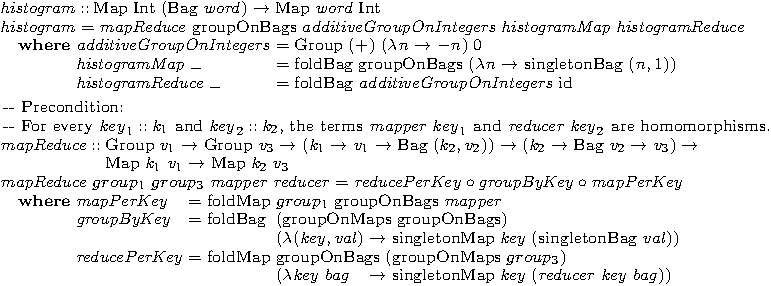
\includegraphics{pldi14/fig-mapReduce.pdf}
\caption{The $\Gl$-term $\HISTOGRAM$ with Haskell-like syntactic
  sugar. $\Term{additiveGroupOnIntegers}$ is the abelian group induced on
  integers by addition $(\mathbb{Z}, +, 0, -)$.}
\label{fig:case-study-pseudocode}
\end{figure*}

  
For base types with no known incrementalization strategy,
the precise interfaces for differentiation and
proof plugins can guide the implementation effort. These
interfaces could also from the basis for a library of
differentiation plugins that work well together.

Rewriting whole programs in our language would be an excessive
requirements. Instead, we embed our object language as an EDSL in
some more expressive meta-language (Scala in our case study), so
that embedded programs are reified. The embedded language can be
made to resemble the metalanguage~\citep{rompf2010lightweight}.
To incrementalize a part of a computation, we write it in our
embedded object language, invoke $\DERIVE$ on the embedded
program, optionally optimize the resulting programs and finally
invoke them. The metalanguage also acts as a macro system for the
object language, as usual. This allows us to simulate polymorphic
collections such as $\Bag*[\Gi]$ even though the object language is
simply-typed; technically, our plugin exposes a family of base
types to the object language.

\pg{Explain how we construct changes? The metalanguage can then
  construct changes in different ways?}



  \begin{oldSec}
\subsection{Methodology}
\label{ssec:methodology}


\begin{itemize}
\item We identify (classes of) base types which are relevant for
  our application, together with any relevant equational properties.
\item We define change representations for these base
  types.
\pg{Here we should give some criteria, if we can.}
\pg{For instance, restrictions on change structures which are
  erased become additional invariant for the change types.}
\pg{For instance, we should
  discuss the point of this paragraph:
``Furthermore, derivatives need to inspect the intensional
structure of changes, which are typically small, without applying
them to their base value, which is typically big. The interface
to do this depends on the specific change structure, hence we
specify no generic operation to allow this.''
}
\item We design for each (class of) base type a relevant set of
  primitives.  Where
  useful, we provide optimized derivatives for such primitives.
  We try to define primitives which capture
  incrementalizable computation skeletons; if such primitives are
  not general enough, we can add additional primitives which are
  more general but whose derivatives are less efficient.
\item We transform target programs to use our primitives.
\end{itemize}

\pg{I need self-maintainability and predicting nil changes here
  to discuss the example. So maybe the example should just be
  part of the case study.}
For instance, \citet{GlucheGrust97Incr} incrementalize bags for a
first-order language. By adapting/extending those techniques, we
can integrate bags into our higher-order language.

\pg{We should say dictionary, not map, for reduced ambiguity with the map operation.}
Using similar techniques, we also implemented support for the
operation on maps needed in our case study.

\pg{This section should also explain where changes come from.}
\end{oldSec}



\subsection{Predicting nil changes}
Handling changes to all inputs can induce excessive overhead in incremental
programs~\citep{Acar09}. It is also often
unnecessary; for instance, the function argument of $\Term{fold}$ in 
\cref{sec:intro} does not change since it is a closed subterm of the program, so
$\Term{fold}$ will receive a nil change for it.
A (conservative) static analysis can detect changes that are guaranteed to be nil at runtime. 
We can then specialize derivatives that receive this change, so that they need not
inspect the change at runtime.

For our case study, we have implemented a simple static analysis which
detects and propagates information about closed terms. The analysis is not interesting and 
we omit details for lack of space.



% Emacs, this is -*- latex -*-!

\subsection{Self-maintainability}
\label{sec:performance-cons}
\label{ssec:self-maint}

\begin{oldSec}
On its own, deriving $\Gl$-abstractions, applications and
variables (\cref{fig:correctness:derive}) does not improve performance.
It only relates the computations embodied in the primitives in
an incremental and higher-order setting, and provides a method to
generalize the vast quantity of research on first-order incremental
computation in the field of databases.
Our first approach toward performance gain is based on the idea of \emph{self-maintainable uses of primitives};
other approaches are certainly feasible. We did not formalize the
optimizations or prove them correct.
\end{oldSec}

In databases, a self-maintainable view~\citep{Gupta99MMV} is a function that can
update its result from input changes alone, without looking at
the actual input. By analogy, we call a derivative
\emph{self-maintainable} if it uses no
base parameters, only their changes. Self-maintainable derivatives
describe efficient incremental computations: since they do not
use their base input, their running time does not have to depend on the input
size.

\begin{examples}
$\Derive{\MERGE} = \Lam {x\; \D x\; y \; \D y}{\Merge{\D x}{\D y}}$
is self-maintainable with the
change structure $\ChangeStruct{\Bag{S}}$ described in
\cref{ssec:change-structures}, because it does not use the base
inputs $x$ and $y$.
Other derivatives are self-maintainable only in certain contexts.
The derivative of element-wise function application
$\App*{\App\MAP f}{\mathit{xs}}$ ignores the original
value of the bag $\mathit{xs}$ if the changes to
%
$f$ are always nil, because the underlying primitive $\FOLDBAG$
is self-maintainable in this case (as discussed in next section).
%
We take advantage of this by implementing a specialized
derivative for $\FOLDBAG$.

We have seen in \cref{ssec:differentiation} that $\Derivative$
needlessly recomputes $\Merge\Xs\Ys$. However, the result is a
base input to $\FOLD'$.
%
In next section, we'll replace $\FOLD'$ by a self-maintainable
derivative (based again on $\FOLDBAG$) and will avoid this
recomputation.
\end{examples}

%% Rationale for previous statement. Too complicated; left out.
%deriving a closed term without primitives yields a term that is
%self-maintainable whenever its higher-order arguments receive
%self-maintainable changes.
%The default rule $\Derive{c} = \Diff c c$ does not yield
%self-maintainable derivatives, because $\DIFF$ and $\APPLY$ use
%the input~$x$ in a significant way (\cref{fig:diff-apply}).
%However,

To conservatively predict whether a derivative is going to be
self-maintainable (and thus efficient), one can inspect whether
the program restricts itself to (conditionally) self-maintainable
primitives, like $\MERGE$ (always) or $\MAP \APP f$ (only if $\D
f$ is nil, which is guaranteed when $f$ is a closed term).

%% From the author response.
%It is possible to give a conservative approximation of whether a program's derivative is self-maintainable:
%If the original program only uses primitives with fully
%self-maintainable derivatives, the derivative of the program will
%be self-maintainable, too. We can syntactically approximate full
%self-maintainability of a primitive by checking whether the code
%of its derivative uses the $x$ variable (in addition to $\D x$) \pg{bind x! What about multiple arguments?}. For
%instance, the derivative of $\MERGE$ uses only $\D x$ and $\D y$, never $x$
%or $y$, and is hence fully self-maintainable. The derivative of
%$\FOLDBAG$ uses both $f$ and $\D f$; it is only self-maintainable
%sometimes (when df is the nil change).

\begin{oldSec}
Sometimes we can safely replace the derivative of a primitive by
a self-maintainable term, in which case we call it a
\emph{self-maintainable use of a primitive.}
Terms have self-maintainable derivatives if they use
primitives in a self-maintainable manner.

\pg{As Klaus points out, this is not true until we fix the set of
  changes - discussed in \#265. So we should specify the set of
  changes, or use a different example. We should also motivate
  it.}
%
\pg{Agreed: Convert to bags and to our running example, using foldBag.}
To illustrate, suppose $\MAP$ is a primitive of sets of
integers,
and changes to sets consist of insertions and deletions only.
The term
\[
\Lam x {\MapT {\Lam*n {n + 1}} x}
\]
contains a self-maintainable use of $\MAP$, because any change to
the input set~$x$, say $\{\App\INSERT5, \App\DELETE7\}$, can be
converted to an output change, say $\{\App\INSERT6,
\App\DELETE8\}$, without looking at $x$ itself. The use of $\MAP$
in the following term is not self-maintainable:
\[
\Lam x {\MapT {\Lam*n {n + \Sum* x}} x}.
\]
Even one insertion to the input set~$x$ generates a sweeping
change over all elements of the output set that is impossible to
express in terms of insertions and deletions without knowledge of $x$.

\pg{Before this, show that some of our primitives are
  self-maintainable, and some are self-maintainable if some
  inputs are nil.}
Our prototype optimization framework proceeds in two steps.
\begin{enumerate}
\item A static analysis identifies when changes are guaranteed to be nil.
\item During the differentiation transformation, $\DERIVE$
selects an appropriate self-maintainable function whenever possible,
considering the results of the static analysis.
\end{enumerate}
Due to space constraint, we cannot go into details of those
steps.
%
\yc{link to code}
%
\end{oldSec}

To avoid recomputing base arguments for self-maintainable derivatives
(which never need them), we
currently employ lazy evaluation.  Since we could use standard techniques for dead-code
elimination~\citep{Appel97} instead, laziness is not central to our
approach.

A significant restriction is that not-self-maintainable derivatives can require expensive computations to supply their base
arguments, which can be expensive to compute. Since they are also
computed while running the base program, one could reuse the previously
computed value through memoization or extensions of static
caching (as discussed in \cref{ssec:staticmemo}). We leave implementing these optimizations for future work. As a consequence,
our current implementation delivers good results only if
most derivatives are self-maintainable.

\begin{oldSec} % ID=Appel97
\pg{Do not remove without universal agreement. I don't think the paper can avoid discussing this aspect. }
One important issue is left. In a call-by-value
implementation of lambda calculus, running the program
\[
\Derive{\App{s}{t}} = \App{\App{\Derive{s}}{t}}{\Derive{t}}
\]
computes $t$
again, even though it was computed in the base program, thus
leading to wasteful repeated computation.
However, we claim this is a simpler problem to solve.
Three possibilities arise:
\begin{enumerate}
\item $t$ is very cheap to compute (for instance, it is a
  literal), so the problem does not occur.
\item $t$ is passed to a function which does not use it, hence
  we can avoid computing it using separate optimization steps, by
  executing the derivative with a lazy semantics (as done in our
  benchmarks) or (we expect) by using known techniques for
  interprocedural dead-code elimination~\citep{Appel97}.
\item Otherwise, since the term $t$
  was already computed while running the base
  program, we can save its value for use in the derivative.
  Approaches to
  implement this include memoization~\pg{cite} and extensions of
  static caching (as discussed in Sec.~\ref{sec:rw}).
  We leave investigating the different
  approaches to future work.
\end{enumerate}
\end{oldSec}

\begin{oldSec} % ID=Gupta99MMV
We next analyze when $t$ is going to be unused.
Inspecting the definition of $\DERIVE$ shows that only derivatives of (functions
containing) primitives can use $t$. For instance,
$\Derive{\Lam{x}{x}} = \Lam{x}{\Lam{\D x}{\D x}}$ does not use its
base input $x$, because $\Derive{x} = \D x$.
\pg{Make this more tentative. Remove 'prove'.}
It's easy to prove
by induction that if derivatives of primitives appearing in $s$
do not use their base input, neither does $s$.\footnote{Function
  changes coming from outside the program are not covered by this
  proof and are possible counterexamples.}

We term primitives whose derivative does not use their base input
self-maintainable, by analogy with the database concept of
self-maintainable views~\citep{Gupta99MMV}. \ko{Give example of 
self-maintainable and non-self-maintainable primitive}. 
We then extend this to programs: a
closed program is self-maintainable if its result does not depend
on base inputs or base intermediate results.
%
For programs which do not depend on functions as parameters (and
whose derivatives hence do not have function changes as
parameters), it should be straightforward to prove that being
self-maintainable is equivalent to only using self-maintainable
primitives.

Hence, we can argue informally that if a program only uses
self-maintainable primitives, its derivative will not recompute
base intermediate results (except if they are computed for
unrelated reasons). In our case study (Sec.~\ref{sec:eval}),
such derivatives are already
extremely efficient.

\pg{This should be somehow better integrated in the rest of the section.}
\end{oldSec}


\subsection{Case study}
\label{sec:plugins}


We perform a case study on a nontrivial realistic program to
demonstrate that \ILC\ can speed it up.
We take the MapReduce-based skeleton of the
word-count example~\citep{Lammel07}. We define a
suitable differentiation plugin, adapt the program to use it and show
that incremental computation is faster than recomputation.
%
We designed and implemented the differentiation plugin 
following the requirements of the corresponding proof plugin,
even though we did not formalize
the proof plugin (e.g. in Agda).
For lack of space, we focus on base types
which are crucial for our example and its performance, that is,
collections.
%
The plugin also implements tuples, tagged unions, Booleans and
integers with the usual introduction and elimination forms, with
few optimizations for their derivatives.

$\WORDCOUNT$ takes a map
from document IDs to documents and produces a map
from words appearing in the input to the count of their
appearances, that is, a histogram:
\[
\HasType \WORDCOUNT {\Fun {\HashMap \DOCUMENTID \DOCUMENT} {\HashMap \WORD \Int}}
\]
For simplicity, instead of modeling strings, we model documents
as bags of words and document IDs as integers. Hence, what we implement is:
\[
\HasType \HISTOGRAM {\Fun {\HashMap \Int {\Bag*[a]}} {\HashMap a \Int}}
\]
We model words by integers ($a = Int$), but treat them parametrically.
Other than that, we adapt directly
\citeauthor{Lammel07}'s code to our language.
\pg{But it cannot accept all the same parameters... Ah, but it
  depends on which foldMap we call. OK.}
\Cref{fig:case-study-pseudocode} shows the $\Gl$-term
$\HISTOGRAM$.

% Emacs, this is -*- latex -*-!
\begin{figure}

\centering

\lstinputlisting[language=scala,
firstline=10,
escapechar=|,
literate=
{=>}{$\Rightarrow\,$}2
{>=}{$\ge\;$}2
{<-}{$\leftarrow\;$}2
{!=}{$\ne\;$}2
{Abelian-group-based}{\text{Abelian-group-based }}1
{<}{$<$}2
{bag1}{{bag$_1$}}4
{bag2}{{bag$_2$}}4
{value1}{{value$_1$}}6
{value2}{{value$_2$}}6
{dict1}{{dict$_1$}}5
{dict2}{{dict$_2$}}5
{v1}{{v$_1$}}2
{v2}{{v$_2$}}2
{???}{$\ldots$}3
]{pldi14/mapReduce.scala}
\caption[A Scala implementation of primitives for bags and maps]{A Scala implementation of primitives for bags and maps.
In the code, we call $\boxplus$, $\boxminus$ and $e$ respectively \emph{merge}, \emph{inverse}, and \emph{zero}.
We also omit the relatively standard primitives.\pg{Can we now move this code to an appendix, since we explain so much in text?}}
\label{fig:primitives}
\end{figure}


\pg{Why does 'target language' show up all of a sudden? Shouldn't
  we say that we generate Scala code for execution
  \textbf{elsewhere}? Right now, we say it in next section. Confusing.}
%
\Cref{fig:primitives} shows a simplified
Scala implementation of the primitives
used in \cref{fig:case-study-pseudocode}.
As bag primitives, we provide constructors and a fold operation,
following \citet{GlucheGrust97Incr}. The constructors for bags
are $\Empty$ (constructing the empty bag), $\SINGLETON$
(constructing a bag with one element), $\MERGE$ (constructing the
merge of two bags) and $\NEGATE$ ($\Negate{b}$ constructs a bag
with the same elements as $b$ but negated multiplicities); all but $\SINGLETON$ represent
abelian group operations.
%
Unlike for usual ADT constructors, the same bag can be
constructed in different ways, which are equivalent by the equations defining abelian groups;
for instance, since $\MERGE$ is commutative, $\Merge{x}{y} = \Merge{y}{x}$.
%
Folding on a bag will represent the bag through constructors in
an arbitrary way, and then replace constructors with arguments;
to ensure a well-defined result, the arguments of fold should
respect the same equations, that is, they should form an abelian group;
for instance, the binary operator should be commutative.
%
Hence, the fold operator $\FOLDBAG$ can be defined to take a
function (corresponding to $\SINGLETON$) and an abelian group
(for the other constructors). $\FOLDBAG$ is then defined by equations:
%
\begin{alignat*}{2}
&  \HasType{\FOLDBAG}{\mathbf{Group}\; \Gt \to (\Gs \to \Gt) \to &&\Bag[\Gs] \to \Gt}\\
&  \App{\FoldBag {g @ (\_, \boxplus, \boxminus, e)}{f}}{\Empty}
    &&= e \displaybreak[0]\\
&  \App{\FoldBag {g @ (\_, \boxplus, \boxminus, e)}{f}}{\Merge* {b_1} {b_2}}
   &&= \App{\FoldBag{g}{f}}{b_1} \displaybreak[0]\\
&&& \boxplus
  \App{\FoldBag{g}{f}}{b_1} \displaybreak[0]\\
&  \App{\FoldBag {g @ (\_, \boxplus, \boxminus, e)}{f}}{\Negate* b}
   && = \boxminus \; \App*{\FoldBag{g}{f}}{b}\displaybreak[0]\\
&  \App{\FoldBag {g @ (\_, \boxplus, \boxminus, e)}{f}}{\Singleton*{v}}
   &&= \App{f}{v}
\end{alignat*}
%
If $g$ is a group,
these equations specify $\App{\FOLDBAG} g$ precisely~\citep{GlucheGrust97Incr}.
%
Moreover, the first three equations mean that $\FoldBag{g}{f}$ is \emph{abelian group
  homomorphism} between the abelian group on bags and the group
$g$ (because those equations coincide with the definition).
%
\Cref{fig:primitives} shows an implementation of $\FOLDBAG$ as
specified above.
Moreover, all functions which deconstruct a bag can be expressed in
terms of $\FOLDBAG$ with suitable arguments.
%
For instance, we can sum the elements of a bag of integers with
$\FoldBag{\Term{gZ}}{\Lam*{x}{x}}$, where
$\Term{gZ}$ is the abelian group on integers defined in
\cref{ssec:change-structures}.
Users of $\FOLDBAG$ can define different abelian groups to specify
different operations (for instance, to multiply floating-point numbers).

If $g$ and $f$ do not change, $\FoldBag{g}{f}$ has a self-maintainable
derivative.
By the equations above,
\pg{Non-standard alignment, because the last line doesn't fit.}
\begin{align*}
& \FoldBag{g}{f} \Update*{b}{\D b}\displaybreak[0]\\
=\;& \FoldBag{g}{f} {(\Merge b {\D b})}\\
=\;& \App{\FoldBag{g}{f}}{b}  \boxplus \App{\FoldBag{g}{f}}{\D b} \\
=\;& \Update{\App{\FoldBag{g}{f}}{b}}{\Term{GroupChange} \; g \; \left(\App{\FoldBag{g}{f}}{\D b}\right)}
\end{align*}
We will describe the $\Term{GroupChange}$ change constructor in a moment.
Before that, we note that as a consequence, the derivative of $\FoldBag{g}{f} $ is
\[
\Lam{b \; db} \Term{GroupChange} \; g \; \left(\App{\FoldBag{g}{f}}{\D b}\right)\text{,}
\]
and we can see it does not use $b$: as desired, it is
\emph{self-maintainable}. Additional restrictions are require to
make $\FOLDMAP$'s derivative self-maintainable. Those restrictions require the
precondition on $\Term{mapReduce}$ in
\cref{fig:case-study-pseudocode}. $\Term{foldMapGen}$ has the
same implementation but without those restrictions; as a
consequence, its derivative is not self-maintainable, but it is more generally applicable.
Lack of space prevents us from giving more details.

To define $\Term{GroupChange}$, we need a suitable erased change
structure on $\Gt$, such that $\UPDATE$ will be equivalent to
$\boxplus$. Since there might be multiple groups on $\Gt$, we
\emph{allow the changes to specify a group}, and have
$\UPDATE$ delegate to $\boxplus$:
\begin{align*}
& \Change{\Gt} = \Term{Replace}\; \Gt \mid \Term{GroupChange} \Abelian*{\Gt} \Gt \\
& \Update{v}{(\Term{Replace} \; u)} = u\\
& \Update{v}{(\Term{GroupChange} \; (\bullet, \Term{inverse}, \Term{zero})\; dv)} = v \bullet dv\\
& \Diff{v}{u} = \Term{Replace}\; v
\end{align*}
That is, a change between two values is either simply the new
value (which replaces the old one, triggering recomputation),
or their difference (computed with abelian group
operations, like in the changes structures for groups from
\cref{ssec:change-structures}. The operator $\DIFF$
does not know which group to use, so it does not take advantage
of the group structure.
However, $\FOLDBAG$ is now able to generate a group change.
% Rewrite:
%derivatives of primitives like $\FOLDBAG$ can
%use the group structure they have available when producing changes.
%
\pg{Clarify about user-defined groups.}

We rewrite $\Program$ in terms of $\FOLDBAG$ to take advantage of
group-based changes.
{\DeriveProgramEnv
\begin{align*}
&\Term{id}=\Lam{x}{x}\\
&G_+ = (\mathbb Z, +, -, 0)\\
&\Program = \Lam{\Xs}{\Lam{\Ys}{\FOLDBAG~G_+~\Term{id}~(\Merge\Xs\Ys)}}\\
&\Derive\Program=\\
&\zero
\Lam{\Xs}{\Lam{\DXs}{}}\Lam{\Ys}{\Lam{\DYs}{}}\\
&\one
\FOLDBAG'~G_+~G_+'~\Term{id}~\Term{id}'\\
&\two
(\Merge\Xs\Ys)\\
&\two
(\MERGE'~\Xs~\DXs~\Ys~\DYs)
\end{align*}
}%
It is now possible to write down the derivative of $\FOLDBAG$.
{\DeriveProgramEnv
\begin{align*}
&\text{(if static analysis detects that $\D G$ and $\D f$
are nil changes)}\\
&\FOLDBAG'=\Derive{\FOLDBAG}=\\
&\zero
\Lam{G}{\Lam{\D G}{\Lam{f}{\Lam{\D f}{
\Lam{\Zs}{\Lam{\DZs}{}}}}}}\\
&\one
\Term{GroupChange}~G~
(\FOLDBAG~G~f~\DZs)
\end{align*}
}%
We know from \cref{ssec:plugin} that
\[
\MERGE'=\Lam{u}{\Lam{\D u}{\Lam{v}{\Lam{\D v}{\Merge{\D u}{\D v}}}}}.
\]
Inlining $\FOLDBAG'$ and $\MERGE'$ gives us a more readable term
$\beta$-equivalent to the derivative of $\Program$:
{\DeriveProgramEnv
\begin{align*}
&\Derive\Program=\\
&\zero
\Lam{\Xs}{\Lam{\DXs}{}}\Lam{\Ys}{\Lam{\DYs}{}}
%
\FOLDBAG~G_+~\Term{id}~
(\MERGE~\DXs~\DYs).
\end{align*}
}%

\begin{oldSec}
Function destructing bags must be homomorphisms between abelian
groups~\citep{GlucheGrust97Incr}, and can all be defined in terms
of $\FOLDBAG$. More in general, bags form an abelian
\emph{collection group}.
%
%To incrementalize bags, we reuse the change structure on bags
%described in \cref{ssec:change-structures}.
%
An abelian group on $\Gi$ can be lifted to an abelian collection
group on $(\HashMap{\kappa}{\Gi})$ through \emph{mapGroup}, so that we
can apply similar ideas to maps. The resulting primitives for map
are expressive enough to efficiently incrementalize our example
program.

Destructing an abelian collection group produces a value in an
abelian group (such as integers or abelian collection groups). To
avoid hardcoding which group to use, we define a general change
structure for abelian groups. After erasure, the change structure is as follows
(cf.~\cref{fig:change-operations,fig:case-study-pseudocode}):\footnote{For clarity, we use ADTs and pattern matching instead of sum types.}
...

The derivative of $\App{\FOLDBAG}{f}$ is efficient on $\Term{Update}$ changes when $df$ is
known to be a nil change; in that case,
$\App{\FOLDBAG}{f}$ is a homomorphism, hence self-maintainable (\cref{sec:performance-cons}). To see why, take any homomorphism $\HasType f {\Fun \Gs \Gt}$ 
between user-defined
abelian groups $G_\Gs$ and $G_\Gt$, and suppose
$\D v = \HasType{\Term{Update} \; (G_\Gs, u)}{\Change \Gs}$. By homomorphism properties,
\begin{align*}
\App f {\Update*{v}{\D v}}
&= \App f {(v \bullet_\Gs u)}
= \App* f v  \bullet_\Gt \App* f u \\
&= \Update{\App* f v}{\Term{Update} \;(G_\Gt, \App f u)}.
\end{align*}
The derivative of $f$ on
$\Term{Update}$ changes is then $\App{\App{f'}{v}}{(\Term{Update} \; (G_\Gs, u))} = \Term{Update} \; (G_\Gt, \App f u)$,
by \cref{def:derivatives}.
$f'$
requires no information about $v$, therefore it is
self-maintainable. That is the
principle behind all derivatives in the plugin that are faster
than recomputation.
\end{oldSec}

\begin{oldSec}
\subsubsection{Bags}

We apply \citeauthor{GlucheGrust97Incr}'s approach to view
maintenance based on monoid- and group-homomorphisms
\citep{GlucheGrust97Incr}. An operation $f$ on a collection is
effectively incrementalized if the collection type forms a group
$G$, and $f$ is a homomorphism from $G$ to some group over its
result type. Bags with signed multiplicities%
%
\footnote{Bags with signed multiplicities correspond to databases
described in \citet{Koch10IQE}, where tuples are allowed to have
negative multiplicities. Bag elements with negative
multiplicities represent deletion of themselves.}
%
form the free abelian group over their element type; their nice
properties are particularly suitable for our purposes.
Incremental computation based on noncommutative groups requires
caching intermediate results, and we leave it for future work.

Bag constructors $\Empty$, $\SINGLETON$, $\MERGE$ are identical
to those used in \citet{GlucheGrust97Incr}. We add a primitive
$\NEGATE$ to create bags with negative multiplicities.
% listing order follows argument order of $\FOLDBAG$.
\begin{align*}
\HasTypeAligned{\MERGE}
  {\Fun{\Fun{\Bag[\Gi]}{\Bag[\Gi]}}{\Bag[\Gi]}}
\\
\HasTypeAligned{\NEGATE}
  {\Fun{\Gi}{\Bag[\Gi]}}
\\
\HasTypeAligned{\Empty}
  {\Bag[\Gi]}
\\
\HasTypeAligned{\SINGLETON}
  {\Fun{\Gi}{\Bag[\Gi]}}
\end{align*}
If we consider $\NEGATE$ to be another bag constructor, then a
natural elimination form of bags is the primitive $\FOLDBAG$:
\begin{align*}
\HasTypeAligned\FOLDBAG
  {\Fun {\Abelian \Gi}
    {\Fun {\Fun*{\Gi}{\Gt}} {\Gt}}}
\\
\Abelian\Gi
  & =      \Fun*{\Base\Gi}{\Fun{\Base\Gi}{\Base\Gi}} \\
  & \times \Fun*{\Base\Gi}{\Base\Gi} \\
  & \times \Base*\Gi.
\end{align*}
\citet{GlucheGrust97Incr} implement many object query language
views in terms of $\FOLDBAG$ to show that they are
homomorphisms and easily incrementalized. Since our framework
supports higher-order functions, we can actually offer
$\FOLDBAG$ to users, who are then free to write all kinds of
easily incrementalized homomorphisms
(\cref{foldBag-homomorphism}).

% Actually, the fact & lemma below talk about functions in the
% semantic domain. Semantic brackets are left out by abusing
% notation.
\begin{definition}[Semantics of bag primitives]~
\begin{subdefinition}
\item $\Eval{\Bag[\Gi]}$ is the free abelian group with basis $\Eval\Gi$.
\item $\MERGE$ evaluates to the binary operator of the free abelian
group.
\item $\NEGATE$ evaluates to the function that takes every
element of $\Eval{\Bag[\Gi]}$ to its inverse in the free abelian
group.
\item $\Empty$ evaluates to the identity element of the free
abelian group.
\item\label{foldBag-homomorphism} If
$\HasType{G_\tau}{\Abelian\tau}$ evaluates to an abelian group,
then for every term $\HasType f {\Fun\Gi\Gt}$, the term
$\App*{\App\FOLDBAG{G_\tau}}{f}$ evaluates to the unique
homomorphism%
\footnote{ The universal property of free abelian groups
guarantees the existence and uniqueness of such a homomorphism. A
constructive proof of the universal property doubles as a
specification of $\FOLDBAG$. } %
from the free abelian group on $\Gi$ to the group denoted by
$G_\tau$.
\end{subdefinition}
\end{definition}

\subsubsection{Maps}

There is no obvious abelian group structure on maps as there is
on bags. However, $\HashMap\Gk\Gi$ can be thought of as (possibly
infinite) vectors over nullable values of type $\Gi$ indexed by
all values of type $\Gk$. It suggests the group structure on maps
as an indexed direct product of a group structure on $\Gi$. The
formulation would be more elegant if there were dependent type
support in the object language.

These are the primitives on maps.
\begin{align*}
\HasTypeAligned\MAKEMAP
  {\Fun\Gk{\Fun\Gi{\HashMap\Gk\Gi}}}
\\
\HasTypeAligned\LOOKUP
  {\Fun\Gk{\Fun{\Map\Gk\Gi}{\Maybe\Gi}}}
\\
\HasTypeAligned\LIFTGROUP
  \Fun{\Abelian\Gi}{\Abelian{\HashMap\Gk\Gi}}
\\
\HasTypeAligned\FOLDMAP
  \Fun{\Abelian\Gi}
    {\Fun{\Abelian\Gt} \\ & \qquad
      {\Fun{ \Fun*\Gk{\Fun\Gi\Gt} }
        {\Fun{\HashMap\Gk\Gi} \Gt}}}
\end{align*}

\begin{definition}[Semantics of map primitives]~
\begin{subdefinition}
\item $\Eval{\Map\Gk\Gi}$ is the set of partial functions from
$\Eval\Gk$ to $\Eval\Gi$ defined only at a finite number of
points.
\item $\MAKEMAP$ evaluates to the function that converts a
key-value pair to the corresponding partial function defined at
1 point.
\item $\LOOKUP$ evaluates to the standard lookup function on
maps.
\item $\LIFTGROUP$ evaluates to a function that maps abelian
groups $G_\Gi$ over $\Eval\Gi$ to the abelian group formed by
direct product of copies of $G_\Gi$ indexed by $\Eval\Gk$. Its
identity element, binary operation and inverse function are the
empty map, map merge and map negation.
\item Given a map $\HasType m {\HashMap\Gk\Gi}$, abelian groups
$G_\Gi$, $G_\Gt$, and a function $\HasType f
{\Fun\Gk{\Fun\Gi\Gt}}$ such that $\App*fk$ is a homomorphism from
$G_\Gi$ to $G_\Gt$ for every $\HasType k\Gk$, the term
\[
\App{\App{\App{\App\FOLDMAP{G_\Gi}}{G_\Gt}}f}m
\]
evaluates to a value in $\Eval\Gt$ by the following steps (we
write $m(k)$ for the value of the map $m$ at key $k$).
\begin{enumerate}
\item Replace each $m(k)$ by $\App*{\App fk}{m(k)}$ to create the
map $\HasType{m'}{\HashMap\Gk\Gt}$.
\item Sum all values of $m'$ by the binary operation of $G_\Gt$.
\end{enumerate}
Since both steps are homomorphisms,
$\App*{\App{\App\FOLDMAP{G_\Gi}}{G_\Gt}}f$ is a homomorphism
from $\App*\LIFTGROUP{G_\Gi}$ to $G_\Gt$.
% to the unique homomorphism%
% \footnote{The existence and uniqueness of such a homomorphism is
% guaranteed by the universal property of indexed direct product
% as a product in the category of abelian groups.} %
% from $\App*\LIFTGROUP{G_\Gi}$ to $G_\Gt$ that agrees with
% $\App*fk$ for every $\HasType k \Gk$.
%
\end{subdefinition}
\end{definition}

Since our object language lacks dependent types, the user has to
make sure that the higher-order argument of $\FOLDMAP$ gives
rise to homomorphisms. This is the price paid for the
expressivity of user-defined groups.

\end{oldSec}
% Below are previous formulations.

% OLDSEC: rephrased skeleton & pointers
\begin{oldSec}
We perform a case study applying our technique to a MapReduce
skeleton. To this end, we implemented in Scala a language plugin
supporting some collections. We restricted ourselves to
primitives whose derivatives could be made self-maintainable.

To this end, we recast and extend some ideas by
\citet{GlucheGrust97Incr} and \citet{Koch10IQE} in our framework.
The collections we consider are maps and bags with negative
multiplicities. We use negative multiplicites to represent
removal of elements.%
%
\footnote{Our framework allows having standard bags as base types
  and bags with negative multiplicities as their change type. We
  leave this and a few other extension for future work.}
%
Bag elements must be comparable for equality, and this excludes
functions. Moreover, storing functions in data is hard because
the derivative of code extracting and using the function must
also have access to the derivative of that function. We plan to
augment base programs to also store function derivatives together
with the functions, but leave this for future work. \pg{Say
  something more.}

\pg{Write instantiation for bags.}
\begin{figure}[h]
\begin{align*}
\Change[\Bag \iota]{b} & = \Bag \iota\\
\Diff[\Bag \iota]{x}{y} & = \Merge x {\Negate*y}\\[\eqsep]
\Apply[\Bag \iota]{\D x}{x} & = \Merge x y
\end{align*}
%\caption{Term difference and change application.}
%\label{fig:plug-diff-apply}
\end{figure}
\end{oldSec}

% OLDSEC: skeleton.
% Refer for ideas.
\begin{oldSec}
We will illustrate a fully instantiated differentiation framework
by the simplest plugin expressive enough for nontrivial
applications. We will not prove the properties required of the
plugin for correctness to hold, but we believe that they are
true.

We designed the plugin around abelian groups.
Abelian groups are good for incrementalizing folds over a
collection because the irrelevance of folding order and the
possibility of removing an element from the fold via its inverse
means that we don't have to save any intermediate result. We
shall not investigate the caching aspect of incrementalization;
we do it later.

Some base types have changes based on abelian groups. Other base
types (sums) don't, but are still useful. Our plugin does not
make everything efficient. We give some primitives fast
derivatives now, and plan to support more and more primitives to
allow more and more fast derivatives.

By the way, we forbid functions in collections because nil
changes to functions have computation content and can't be
discarded. [Illustrating example: Klaus's f]

\subsection*{Details}

Listing: base types, their change types, DIFF, UPDATE

Those fall into 2 categories: those whose change we don't care
about (simply use replacement), and those whose change we care
about (change is either replacement value, or user-supplied
abelian group together with a group element.

Listing: derivatives

We can talk about foldBag and foldMap alone, leaving
everything else the difference with itself (that is, stupid
derivative by recomputation).
\end{oldSec}

% OLDSEC: abelian groups
% Refer to it when discussing AbelianDerivation traits.
\begin{oldSec}
Our approach is parametric in the concrete representation of
changes of type $\Change{\tau}$ as long as changes support the
operations listed in \cref{fig:change-operations}).
The update operator $\Apply{\D x}{x}$ updates a value $x$ with a
change $\D x$. The difference operator $\Diff{y}{x}$ computes the
change from $x$ to $y$.
And the nil change operator $\Nil{x}$
denotes the change that updates the value $x$ into itself.

In fact, if $\tau$ forms a group $\langle \tau, 0, +, -\rangle$,
we can define $\Diff{v_2}{v_1} = v_2 + (- v_1)$; for some groups,
we can use the resulting definition for incremental computation
\pg{not clear what this means yet}, as we will see later.
However, many interesting datatypes do not form groups, such as
functions or lists (\citet{GlucheGrust97Incr} introduce a group
structure for lists, but it is too restrictive\pg{elaborate});
hence we introduce here a more general abstraction, which can be
implemented via groups \pg{reorder this with the previous
  paragraph}.

\pg{I write $\cdot-\cdot$ for a binary operation, but I need something better.}
For instance, we can take $\tau$ to be the set of integers $\bz$. Integers are
the support of the commutative group $(\bz, \cdot + \cdot, 0, -\cdot)$, hence they are equipped
with a difference operation $\cdot-\cdot = \Gl x y. x + (-y)$. We can thus represent
changes for relative numbers with relative numbers: $\Diff{v_2}{v_1} = v_2 -
v_1$.

More formally, take an arbitrary type $\tau$ and values $v_1, v_2$ of
these type. We can describe the difference between these two values
with $\D v = \Diff{v_2}{v_1}$: this evaluates to a change $\D v$ which is
valid for $v_1$. Moreover, we can apply \pg{is this the term to use?} this change to a value
with $\Apply{\D v}v$. We have the guarantee that
$\Apply{\left(\Diff{v_2}{v_1}\right)}{v_1} = v_2$. In general, if we
apply changes to values for which they are not valid, our axioms do
not specify the result. Moreover, our axioms for arbitrary base types
only guarantee that a change $\Diff{v_2}{v_1}$ is valid for $v_1$,
even though, for many implementations of changes, $\Diff{v_2}{v_1}$ is
valid for values other than $v_1$. This is the case in particular if
the base type forms a group and we define changes reusing this group
structure, as we did for integers. In interesting applications, however, changes
are not generated directly by $\DIFF$.

Moreover, if $\D v$ is a valid change, we also have
$\Diff{\left(\Apply{\D v}v\right)}v = \D v$.

Our presentation of the behavior of changes on a datatype forms
an algebraic specification (excluding the concept of validity and
the properties which only apply to valid changes). In particular,
we can define a signature having sorts $\tau$ and $\Change{\tau}$,
the functions from \cref{fig:change-operations}
and equations (or axioms):
\begin{align*}
\Apply{\Diff*{s₂}{s₁}}{s₁} &= s₂\\
\Apply{\Nil{s}}{s} &= s\\
\end{align*}
\pg{Check which ones we have already proven.}

Since this set of axioms is algebraic (that is, purely first
order), we know from universal algebra~\citep{Mitchell1996foundations} that equational reasoning
is sound and complete for all models (implementations) of this
algebraic specification.

Moreover, we can show that those axioms are consistent by
providing models implementing them. \pg{Resume}
%Additionally, we have two implementations of those axioms.
\pg{A couple more axioms need to be checked.}
%
% (s₂ ⊝ (ds ⊕ s₁)) ∘ ds &= s₂ ⊝ s₁ (?)
%
% Special case:
%	(ds ⊕ s) ⊝ s = ds (EDIT: only if ds is valid for s).
%
% Therorems:
%
%s ⊝ s = nil s
%(s₁ ⊝ s₂) ∘ (s₂ ⊝ s₃) = s₁ ⊝ s₃
\end{oldSec}

\subsection{Benchmark results}

Our results show (\cref{fig:graph}) that our program reacts to input changes
in essentially constant time, as expected, hence orders of magnitude faster than
recomputation. Constant factors are small enough that the speedup is apparent on realistic input sizes.

For lack of space, details on benchmarking results and inputs
are available in the extended version of our paper (Appendix A).

Two important lessons from the evaluations are:
\begin{itemize}
\item As anticipated in \cref{ssec:self-maint}, to achieve good performance our current
  implementation requires some form of dead code elimination, such as laziness.
%Either laziness or dead-code elimination is required for
%good performance ().
\item Incrementalization increases code size significantly.
  Analyzing and addressing this increase is left for future work.
\end{itemize}

\begin{figure}
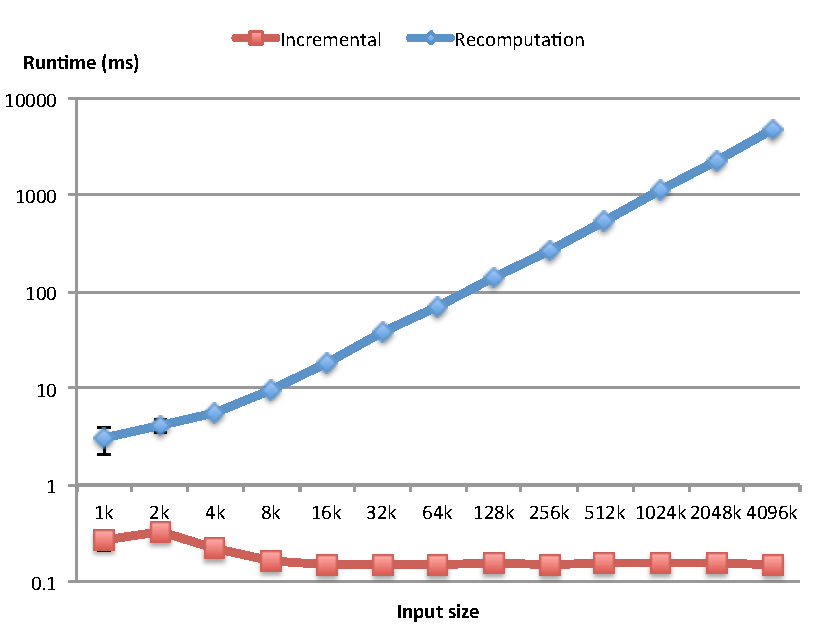
\includegraphics[keepaspectratio,width=8.5cm]{pldi14/HistogramGenerated-new.pdf}
\caption{Performance results in log-log scale, with input size on
  the x-axis and runtime in ms on the y-axis. Confidence
  intervals are shown by the whiskers; most whiskers are
  too small to be visible.}
\label{fig:graph}
\end{figure}

% Emacs, this is -*- latex -*-!
\chapter{Related work}
\label{sec:rw}

Existing work on incremental computation can be divided into two
groups: Static incrementalization and dynamic incrementalization.
Static approaches analyze a program statically and generate an incremental
version of it. Dynamic approaches create dynamic dependency graphs while
the program runs and propagate changes along these graphs.

The trade-off between the two is that static approaches have the potential
to be faster because no dependency tracking at runtime is needed, whereas
dynamic approaches can support more expressive programming languages.
%
\ILC\ is a static approach, but compared to the other static
approaches it supports more expressive languages.

In the remainder of this section, we analyze the relation to the
most closely related prior works. \Citet{Ramalingam93}, \citet{Gupta99MMV}
and \citet{Acar06} discuss further related work.


\section{Dynamic approaches}
One of the most advanced dynamic approach to incrementalization is
self-adjusting computation, which has been applied to Standard ML
and large subsets of C~\citep{Acar09,Hammer11}.
In this approach, programs execute on the original
input in an enhanced runtime environment that tracks the
dependencies between values in a \emph{dynamic
  dependence graph}~\citep{Acar06}; intermediate results are
memoized.
Later, changes to the input propagate through
dependency graphs from changed inputs to results,
updating both intermediate and final results;
this processing is often more efficient than recomputation.

However, creating dynamic
dependence graphs imposes a large constant-factor overhead during
runtime, ranging from 2 to 30 in reported
experiments~\citep{Acar09EAS,Acar10TDT}, and affecting the
initial run of the program on its base input.
\citet{Acar10TDT} show how to support high-level data
types in the context of self-adjusting computation; however, the
approach still requires expensive runtime bookkeeping during the initial run.
Our approach, like other static ones, uses a standard runtime
environment and has no overhead
during base computation, but may be less efficient when processing
changes. This pays off if the initial input is 
big compared to its changes.


\citet{Chen11} have developed a static transformation for purely
functional programs, but this transformation just provides a superior interface to use
the runtime support with less boilerplate, and does not reduce
this performance overhead. Hence, it is still a dynamic approach, unlike
the transformation this work presents.

Another property of self-adjusting computation
is that incrementalization is only efficient if the program has a suitable
computation structure. For instance, a program
folding the elements of a bag with a left or right fold will not
have efficient incremental behavior; instead, it's necessary that
the fold be shaped like a balanced tree. In general,
incremental computations become efficient only if they are \emph{stable}~\citep{Acar05}.
Hence one may need to massage the program to make it efficient. Our methodology is 
different: Since we do not aim to incrementalize arbitrary programs written in standard
programming languages, we can select primitives that have efficient derivatives and thereby require 
the programmer to use them.

Functional reactive programming \citep{Elliott:1997:FRA:258948.258973}
can also be seen as a dynamic approach to incremental computation;
recent work by \citet{Maier2013} has
focused on speeding up reactions to input changes by making them
incremental on collections. \citet{Willis08} use dynamic techniques
 to incrementalize JQL queries.

\section{Static approaches}
\pg{If we discuss partial evaluation, we should compare to
  \citep{Sundaresh91}}
Static approaches analyze a program at compile-time and produce an
incremental version that efficiently updates the output
of the original program according to changing inputs.

Static approaches have the potential to be more efficient than dynamic approaches,
because no bookkeeping at runtime is required. Also, the computed incremental
versions can often be optimized using standard compiler techniques
such as constant folding or inlining.
However, none of them support first-class functions; some
approaches have further restrictions.

Our aim is to apply static incrementalization to more expressive languages;
in particular, \ILC\ supports first-class functions and an open
set of base types with associated primitive operations.

\subsection{Finite differencing}
\label{sec:finite-diff}
\citet{Paige82FDC} present derivatives for a first-order language
with a fixed set of primitives.
\citet{Blakeley:1986:EUM} apply these ideas to a class of relational queries.
The database community extended
this work to queries on relational data, such as in \emph{algebraic
  differencing}~\citep{Gupta99MMV}, which inspired our work and
terminology. However, most of this work does not apply to nested
collections or algebraic data types, but only to relational
(flat) data, and no previous approach handles first-class
functions. Incremental support is typically designed
monolithically for a whole language, rather than piecewise.
Improving on algebraic differencing, \citet{Koch10IQE}
\emph{guarantees} asymptotic speedups with a compositional query
transformation and delivers huge speedup in realistic benchmarks,
though still for a first-order database language.
\pg{continue with new work, discuss why we don't do iterated differentiation.}

More general (non-relational) data types are considered in the work by \citet{GlucheGrust97Incr};
our support for bags and the use of groups is inspired by their work,
but their architecture is still rather restrictive: they lack
support for function changes and restrict incrementalization to
self-maintainable views, without hinting at a possible solution.

\subsection{Static memoization}
\label{ssec:staticmemo}
\citeauthor{Liu00}'s work~\citep{Liu00} allows to incrementalize a first-order base
program $f(\Old{x})$ to compute $f(\New{x})$, knowing how
$\New{x}$ is related to $\Old{x}$. To this end, they transform
$f(\New{x})$ into an incremental program which reuses the
intermediate results produced while computing $f(\Old{x})$, the
base program. To this end, (i) first the base program is
transformed to save all its intermediate results, then (ii) the
incremental program is transformed to reuse those intermediate
results, and finally (iii) intermediate results which are not
needed are pruned from the base program. However, to reuse
intermediate results, the incremental program must often be
rearranged, using some form of equational reasoning, into some
equivalent program where partial results appear literally. For
instance, if the base program $f$ uses a left fold to sum the
elements of a list of integers $\Old{x}$, accessing them from the
head onwards, and $\New{x}$ prepends a new element $h$ to the
list, at no point does $f(\New{x})$ recompute the same results.
But since addition is commutative on integers, we can rewrite
$f(\New{x})$ as $f(\Old{x}) + h$. The author's CACHET system will
try to perform such rewritings automatically, but it is not
guaranteed to succeed. Similarly, CACHET will try to synthesize
any additional results which can be computed cheaply by the base
program to help make the incremental program more efficient.

Since it is hard to fully automate such reasoning, we move
equational reasoning to the plugin design phase. A 
plugin provides general-purpose higher-order primitives for which
the plugin authors have devised efficient derivatives (by using
equational reasoning in the design phase). Then, the
differentiation algorithm computes incremental
versions of user programs without requiring further user intervention.
It would be useful to combine \ILC\ with some form of static
caching to make the computation of derivatives which
are not self-maintainable more efficient. We plan to do so
in future work.
%Our approach is instead fully automatic, and will always produce
%a result, which in the worst case will merely be slow;
%% they can also fail and then 'produce a slow program'.
%
%we envision the use of directed rewrite rules for further
%optimization of programs, instead of undirected search.
%% Not so important.

\chapter{Conclusion}
\label{ssec:future}
In this part we have presented \ILC, an approach to lifting incremental computations
on first-order programs to incremental computations on higher-order
programs. We have presented a machine-checked correctness proof 
of a formalization of \ILC\ and an initial experimental evaluation
in the form of an implementation, a sample plugin for maps and bags,
and a non-trivial example that was incrementalized successfully and
efficiently. 

\pg{Revise}
Our work opens several avenues of future work. Our current implementation
is not efficient on derivatives that are not self-maintainable.
However, as discussed
(Sec.~\ref{ssec:self-maint}), we will study how
to memoize intermediate results to address this limitation. Our next
step will be to develop language plugins which
have efficient non-self-maintainable primitives.

Another area of future work is adding support for algebraic data
types (including recursive types), polymorphism, subtyping, general recursion
and other collection types. While support for algebraic data
types could subsume support for specific collections, many
collections have additional algebraic properties that enable faster
incrementalization (like bags). Even lists (which have fewer algebraic properties)
can benefit from special support~\citep{Maier2013}.

Moreover, we intend to apply \ILC{} to optimize queries on
collections in the context of the \textsc{SQuOpt}
project~\citep{GiarrussoAOSD13}, which was a motivation for this
work; in particular, \textsc{SQuOpt} can automatically rewrite
queries to use database-style indexes, and \ILC{} enables
updating those indexes when input data changes.

\begin{oldSec}
Our derivatives accept arbitrary changes for all inputs. We plan
to stage the code that updates the inputs through lightweight
modular staging~\citep{rompf2010lightweight}, analyze it to
predict changes and specialize the derivative to the result of
this analysis. For instance, if we need to update $\Term{f} \;
\Term{bag}$ after $\Term{bagNew} = \Term{insert} \; \Term{el} \;
\Term{bagOld}$, we can infer that $\Term{dbag}$ is an insertion
and specialize $f'$ to such a change.
\end{oldSec}

Finally, we intend to perform a full and thorough experimental evaluation
to demonstrate that \ILC\ can incrementalize large-scale practical programs.


% Appendixes, to integrate.
% % Emacs, this is -*- latex -*-!
\section{Benchmarks}
% Disabled since we shouldn't refer to this appendix, it's just
% part of the extended version of the paper.
%\label{sec:benchmarks}

Benchmarking our case study shows
that \ILC\ can offer order-of-magnitude speedups for a
realistic higher-order program.

\begin{oldSec} % ID=Adaptation
We performed additional microbenchmarks on simpler examples
(summing the values of a map\pg{Cai: why not the elements of a
  bag?}, mapping the successor function on bag elements, bag
merge);\pg{the examples are really small, is it OK? I guess so.}
results on those examples did not yield additional insight, hence
we omit them from this report.\pg{Add the links for details?}

\paragraph{Adaptation}
We first adapted our example program to our object language,
as parameterized by the plugin we presented in
Sec.~\ref{sec:plugins}. Where primitives were insufficient, we
added new ones as appropriate~\pg{Ensure we don't contradict this
  claim elsewhere.}.

First, we adapted the generic MapReduce framework as a library of
polymorphic object-level functions. As usual, we use the
meta-language both to define the library and to encode
polymorphism.

This produces a more restrictive variant of MapReduce. \pg{Explain.}

Future work, supporting non-self-incrementalizable primitives through caching, would allow lifting these limitations.

The result is shown in \cref{fig:case-study-pseudocode}.
\end{oldSec}

\paragraph{Benchmarking setup}
\pg{Omit this at least while we lack space.}
\begin{oldSec}
We ran benchmarks on an 8-core Intel Core i7-2600 CPU running at
3.4 GHz, with 8GB of RAM, running Scientific Linux release 6.4.
While the benchmark code is single-threaded, the JVM offloads
garbage collection to other cores. We use the preinstalled
OpenJDK 1.7.0\_25 and Scala 2.10.2.
\end{oldSec}

We run object language programs by generating corresponding Scala code.
To ensure rigorous
benchmarking~\citep{Georges07rigorousJavaPerformance}, we use the
Scalameter benchmarking library. To show that the performance
difference from the baseline is statistically significant, we
show 99\%-confidence intervals in graphs.

We verify \cref{eq:correctness} experimentally
by checking that the two sides of the equation always
evaluate to the same value.

\paragraph{Input generation}

Inputs are randomly generated to resemble English words over all
webpages on the internet: The vocabulary size and the average
length of a webpage stay relatively the same, while the number of
webpages grows day by day. To generate a size-$n$ input of type
$(\HashMap{\Int}{\Bag*[\Int]})$, we generate $n$ random numbers
between 1 and 1000 and distribute them randomly in $n/1000$ bags.
Changes are randomly generated to resemble edits. A change has
50\% probability to delete a random existing number, and has 50\%
probability to insert a random number at a random location.

\paragraph{Experimental units}

Thanks to \cref{eq:correctness}, both recomputation
$\App{f}{\Apply*{\D a}{a}}$ and incremental computation
$\Apply{\App{\App{\Derive{f}}{a}}{\D a}}{\App{f}{a}}$ produce
the same result. Both programs are written in our object language.
To show that derivatives are faster, we compare
these two computations. To compare with recomputation, we measure the
\emph{aggregated} running time for running the derivative on the change 
and for updating the original output with the result of the derivative.

\subsection{Experimental results}

\pg{Warning: benchmark results are hardcoded here, copy-pasted
  from the spreadsheet. Edit with care.}

We present our results in \cref{fig:graph}. As expected, the
runtime of incremental computation is
\emph{essentially constant} in the size of the input, while the runtime
of recomputation is linear in the input size.
Hence, on our biggest inputs\pg{specify} incremental computation
is over $10^4$ times faster.

Derivative time is in fact slightly irregular for the first few inputs,
but this irregularity decreases slowly with increasing warmup
cycles. In the end, for derivatives we use $10^4$ warmup cycles.
With fewer warmup cycles, running time for derivatives decreases
significantly during execution, going from 2.6ms for $n = 1000$ to
0.2ms for $n = 512000$. Hence, we believe extended warmup is
appropriate, and the changes do not affect our general
conclusions. Considering confidence intervals, in our experiments the running
time for derivatives varies between 0.139ms and 0.378ms.

In our current implementation, the code of the generated derivatives can become 
quite big. For the histogram example (which is around 1KB of code), a pretty-print
of its derivative is around 40KB of code. The function application case
in \cref{fig:correctness:derive} can lead to a quadratic growth in the 
worst case. We believe that the code size of the derivative can be reduced again 
by common subexpression elimination, but we did not yet pursue that option.

\paragraph{Summary}
Our results show that the incrementalized program runs
in essentially constant time and hence orders of magnitude faster than
the alternative of recomputation from scratch. 

% \section{Addendum: change equality}
\label{sec:change-eq}

While preparing the final version of the paper, we introduced a
small technical mistake: in \cref{thm:deriv-nil}, we assert that
two changes are equal, even though in
\cref{ssec:change-structures} we promised that ``Throughout
our theory, we only discuss equality of base values, not of
changes.''

However, by that time, we had formalized in Agda the correct
equivalence relation to use on change, that we call
delta-observational equivalence (d.o.e.). Intuitively, two
changes are d.o.e. if using them as changes gives the same
observations, as long as we only observe base values and not
changes themselves; below we show the theorems that we have
proved in Agda and that substantiate this intuition, at least to
a great extent.

In this section, we
state the corrected version of \cref{thm:deriv-nil}, and explain
what we know about this change equivalence.

\begin{definition}[Delta-observational equivalence]
  Given a change structure $\ChangeStruct{V}$, a value $v \in V$,
  and two changes $\D v_1, \D v_2 \in \Change{v}$, if and only if
  $\Update{v}{\D v_1} = \Update{v}{\D v_2}$ we say that $\D v_1$
  is delta-observationally equivalent (d.o.e.) to $\D v_2$, and
  we write $\D v_1 \Doe \D v_2$.
\end{definition}

Using this relation, we can state a correct version of
\cref{thm:deriv-nil}:

\begin{lemma}[Behavior of derivatives on $\NILC$]
  \label{thm:deriv-nil-2}
  Given change structures $\ChangeStruct{A}$ and
  $\ChangeStruct{B}$, a function $f \in A \to B$, an element $a$
  of $A$, and the derivative $f'$ of $f$, we have
  $\App{\App{f'}{a}}{\NilC{a}} \Doe \NilC{\App* f a}$.
\end{lemma}

Moreover, we have a number of lemmas about delta-observational
equivalence.

\pg{Revise statements for clarity.}

\begin{lemma}[D.o.e. is an equivalence]
  For any $x \in X$ with a change structure on $X$, d.o.e. is an
  equivalence relation (reflexive, symmetric, transitive) among
  elements of $\Change{x}$.
\end{lemma}

\begin{lemma}[Identities using d.o.e.]
  Using d.o.e. we can state additional algebraic equivalences,
  that complement \cref{def:update-diff}.

\begin{align*}
\Update x \D{x} = x &\Leftrightarrow \D{x} \Doe \NilC{x}\\
\Diff x x &\Doe \NilC {x}\\
\Diff {\Update*{x}{\D{x}}} x &\Doe \D{x}
\end{align*}
\end{lemma}

\begin{lemma}[Function change application preserves d.o.e.]
  For each $x \in X$, with a change structure on $X$, changes
  $\D{x}_1, \D{x}_2 \in \Change{x}$, for each $f \in X \to Y$,
with a change structure on $Y$, and changes
$\D{f}_1, \D{f}_2 \in \Change{f}$, then $\D{f}_1 \Doe \D{f}_2$ and
$\D{x}_1 \Doe \D{x}_2$ imply
$\D{f}_1~x~\D{x}_1 \Doe \D{f}_2~x~\D{x}_2$.
\end{lemma}

That is, in all simple contexts that we can construct, two d.o.e.
changes will behave indistinguishably. In fact, for programs that
only use changes as changes (without looking at their
implementation details), we conjecture that d.o.e. changes are
observationally equivalent. However, making this conjecture
precise and proving it are efforts left for future work.

\begin{lemma}[Extensionality for d.o.e.]
  If two function changes $\D{f}_1, \D{f}_2$ behave equally when
  applied to arbitrary type-correct inputs $x$,
  $\D{x}_1, \D{x}_2 \in \Change{x}$, then $\D{f}_1 \Doe \D{f}_2$.
\end{lemma}

\begin{lemma}[Derivatives are unique up to d.o.e.]
  If two function changes $\D{f}_1, \D{f}_2$ are derivatives for
  $f$, then they're d.o.e. to each other and to $f$'s nil change:
  $\D{f}_1 \Doe \NilC{f} \Doe \D{f}_2$.
\end{lemma}
We only have such an uniqueness theorem up to d.o.e., not to
standard equality, since multiple d.o.e. changes can be
different.
% XXX continue: Transcribe lemmas from Base.Change.Equivalence


\begin{oldSec}
% Emacs, this is -*- latex -*-!
\section{Correctness proof of derivation on simply typed lambda
  terms}
\label{sec:STLC-correct}

\yc{claim correspondence to Agda script}
\pg{Lots of this should move to earlier in the paper, and should not be repeated here. Remember to update this section.}
Let $\GD\Gs$ be the type of changes to values of type $\Gs$. Let
us specify $\GD\Gs$ recursively thus:
\begin{align*}
\GD(\Gs\r\Gt)&=\Gs \r \GD\Gs \r \GD\Gt,\\
\GD\Gi&=\Gi.
\end{align*}
Intuitively, the change to a function is a function computing
changes on the result values, and the change to an individual is
its replacement.
We chose the type of changes $\GD\Gi$ to an individual for
simplicity of presentation; its triviality does not hide the
technical issues associated with derivatives.

As seen before \yc{link to justification},
the derivative of a function of type $(\Gs\r\Gt)$ has the type
$\GD(\Gs\r\Gt)=\Gs\r\GD\Gs\r\GD\Gt$.
Let $\Derive{\cdot}$ be the program transformation that produces
derivatives from terms. Below is the most obvious
\pg{I do not like ``obvious'' here} type-correct
implementation.
\begin{align*}
\Derive{\Lit{k_n}}     & = \Lit{k_n}\\
\Derive{\Var{x^\Gs}}   & = \Var{\D x^{\GD\Gs}}\\
\Derive{\App{s}{t}}    & = \App{\App{\Derive{s}}{t}}{\Derive{t}}\\
\Derive{\Lam{x^\Gs}{t}}& = \Lam{x^\Gs}{\Lam{\D x^{\GD\Gs}}{\Derive{t}}}
\end{align*}
Here $\D x^{\GD\Gs}$ is a fresh variable chosen deterministically
according to $x^{\Gs}$. Henceforth the deterministic choice of
$\D x^{\GD\Gs}$ will be taken for granted.

The most obvious program transformation turns out to be the
correct one.

\begin{theorem}
\label{thm:STLC-correct}
Let $s$ be a closed term of type $(\Gs\r\Gt)$, let $t_0,t_1$ be
closed terms of type $\Gs$, and let $\D t$ be a closed term of
type $\GD\Gs$ denoting the change from $t_0$ to $t_1$. Then we
can obtain the new result $\App* s {t_1}$ by applying the change
$\App*{\App{\Derive s}{t_0}}{\D t}$ to the old result
$\App* s {t_0}$.
\end{theorem}

We need the concepts of difference and change application in
order to make theorem~\ref{thm:STLC-correct} precise and
eventually to prove it.

\begin{definition}
\label{def:diff+apply}
Suppose $u,v\in D_\Gs$ and $\D v\in D_{\GD\Gs}$. Write
$\Diff u v$ for the change from $v$ to $u$, and write
$\Apply{\D v}v$ for the result of applying the change $\D v$ to
the value $v$. The operators $\DIFF$ and $\APPLY$ are defined
recursively as follows, over all $w\in D_{\Gt}$ and
$\D w\in D_{\GD\Gt}$:
\begin{align*}
\Diff u v &= u
&&\text{if}& \Gs&=\Gi\\
\Diff* u v(w)(\D w) &= \Diff{u(\Apply{\D w}w)}{v(w)}
&&\text{if}& \Gs&=(\Gt\r\Gt')\\
\Apply{\D v}v &= \D v
&&\text{if}& \Gs&=\Gi\\
\Apply*{\D v}v(w) &= \Apply{\D v(w)(\Diff w w)}{v(w)}
&&\text{if}& \Gs&=(\Gt\r\Gt')\\
\end{align*}
\end{definition}

With the symbols $\DIFF$ and $\APPLY$, the conclusion of
theorem~\ref{thm:STLC-correct} may be stated succinctly thus:
\[
\mean{\App s {t_1}} =
\Apply{\mean{\App{\App{\Derive s}{t_0}}{\D t}}}
      {\mean{\App s {t_0}}}.
\]
It will be proved via a logical relation that we shall call the
validity of changes.

\begin{definition}[validity of changes]
\label{def:valid-changes}
~ % to push the bullets down
\begin{itemize}
\item Every individual in $D_\Gi$ is a valid change to every
other individual in $D_\Gi$.
\item A function $\D f\in D_{\Gs\r\GD\Gs\r\GD\Gt}$ is a valid
change to the function $f\in D_{\Gs\r\Gt}$ if for every value
$v\in D_\Gs$ and every change $\D v$ valid to $v$,
\begin{enumerate}[(1)]
\item the result $\D f(v)(\D v)$ is a valid change to $f(v)$, and
\item we have
\[
\Apply*{\D f}f \Apply*{\D v}v = \Apply{\D f(v)(\D v)}{f(v)}.
\]
\end{enumerate}
\end{itemize}
\end{definition}

\begin{lemma}
\label{lem:apply-diff}
$
u = \Apply{\Diff* u v}v
$
for all $u,v\in D_\Gs$.
\end{lemma}

\begin{proof}
By induction on the type $\Gs$.

\Case \Gs = \Gi:
By definition
$
  \Apply{\Diff* u v}v
= \Apply uv
= u
$.

\Case \Gs = \Gt \r \Gt': Choose arbitrary $w\in D_\Gt$. Induction
hypothesis on $\Gt$ and $\Gt'$ gives us
\begin{align*}
w    & = \Apply{\Diff* w w}w,\\
v(w) & = \Apply{\Diff*{u(w)}{v(w)}}{v(w)}.
\end{align*}
As a result,
\begin{align*}
\Apply*{\Diff* u v}v(w)
& = \Apply{\Diff*{u(\Apply{\Diff*ww}w)}{v(w)}}{v(w)}\\
& = \Apply{\Diff*{u(w)}{v(w)}}{v(w)}\\
& = u(w).
\end{align*}
Since $w$ is chosen arbitrarily, $\Apply{\Diff* u v}v$ and
$u$ are equal as functions.
\end{proof}

\begin{lemma}
\label{lem:diff-is-valid}
$\Diff* u v$ is a valid change to $v$ for all $u,v\in D_\Gs$.
\end{lemma}

\begin{proof}
By induction on the type $\Gs$.

\Case \Gs = \Gi: Every individual is a valid change to every
other individual.

\Case \Gs = \Gt \r \Gt': Let $w$ be an arbitrary element in
$D_\Gt$ and let $\D w$ be a valid change to $w$. By induction
hypothesis on $\Gt'$,
\[
\Diff* u v(w)(\D w) = \Diff{u(\Apply{\D w}w)}{v(w)}
\]
is a valid change to $v(w)$, fulfilling condition~(1) of the
validity of $\Diff*uv$ as a change to $v$. By
lemma~\ref{lem:apply-diff},
\begin{align*}
u & = \Apply{\Diff*uv}v,\\
u(\Apply{\D w}w)
& = \Apply{\Diff*{u(\Apply{\D w}w)}{v(w)}}{v(w)}.
\end{align*}
They give us
\begin{align*}
    \Apply*{\Diff*uv}v(\Apply{\D w}w)
& = u(\Apply{\D w}w)\\
& = \Apply{\Diff*{u(\Apply{\D w}w)}{v(w)}}{v(w)}\\
& = \Apply{\Diff*uv(w)(\D w)}{v(w)},
\end{align*}
which is precisely condition~(2) of the validity of
$\Diff*uv$ as a change to $v$.
\end{proof}

\begin{definition}
\label{def:consistent-env}
An environment $\Gr$ is consistent if for every variable $x^\Gs$,
the value $\Gr(\D x^{\GD\Gs})$ (with the name $\D x^{\GD\Gs}$
chosen as in $\DERIVE$) is a valid change to $\Gr(x^\Gs)$.
\end{definition}

\begin{definition}[updated environment]
\label{def:updated-env}
If $\Gr$ is a consistent environment, its updated version $\Gr'$
is obtained by setting
\[
\Gr'(x^\Gs) = \Apply{\Gr(\D x^{\GD\Gs})}{\Gr(x^\Gs)}
\]
over all variables $x^\Gs$.
\end{definition}

\begin{lemma}
\label{lem:STLC-valid-correct}
Let $t$ be a term of type $\Gs$, let $\Gr$ be a consistent
environment and let $\Gr'$ be the updated version of $\Gr$.
\begin{enumerate}[(1)]
\item
$\mean*[\Gr]{\Derive t}$ is a valid change to $\mean*[\Gr]t$.
\item
$
\mean[\Gr']t = \Apply{\mean*[\Gr]{\Derive t}}{\mean*[\Gr]t}
$.
\end{enumerate}
\end{lemma}

\begin{proof}
By induction on term structure of $t$.
% In fact we induce on typing judgements.

\Case t = \Lit{k_n}:
Both parts of the lemma are obvious.

\Case t = \Var{x^\Gs}:
We have $\Derive{x^\Gs}=\D x^{\GD\Gs}$. Part~(1) of the lemma
follows from consistency of $\Gr$ and part~(2) from the
definition of updated environments.

\Case t = \App{s_0}{s_1}:
\[
\Derive{t}=\App{\App{\Derive{s_0}}{s_1}}{\Derive{s_1}}.
\]
To avoid clutter, let us write:
\begin{align*}
  f  & = \mean[\Gr]{s_0} &
  f' & = \mean[\Gr']{s_0} &
\D f & = \mean[\Gr]{\Derive{s_0}}\\
  v  & = \mean[\Gr]{s_1} &
  v' & = \mean[\Gr]{s_1} &
\D v & = \mean[\Gr]{\Derive{s_1}}.
\end{align*}
Then
\[
\mean[\Gr]{\Derive{t}} = \D f(v)(\D v).
\]
By induction hypothesis, $\D f$ is a valid change to $f$, and $\D
v$ is a valid change to $v$. By the definition of validity of
changes, $\D f(v)(\D v)$ is a valid change to $f(v)$ and part~(1)
holds. For part~(2), observe that the induction hypothesis on
$s_0$ and $s_1$ gives us
\begin{align*}
f' &= \Apply{\D f}{f},&
v' &= \Apply{\D v}{v}.
\end{align*}
By validity of $\D f$ to $f$:
\begin{align*}
\mean[\Gr']{t}
& = f'(v') \\
& = (\Apply{\D f}f)(\Apply{\D v}{v}) \\
& = \Apply{\D f(v)(\D v)}{f(v)} \\
& = \Apply{\mean*[\Gr]{\Derive t}}{\mean*[\Gr]t}.
\end{align*}

\Case t = \Lam{x} s:%
Suppose $\Gs\r\Gt$ is the type of $t$. Choose arbitrary $v\in
D_\Gs$ and let $\D v$ be a valid change to $v$. Define these
shorthands:
\begin{align*}
f     & = \mean[\Gr]{\Lam{x} s} \\
\D f  & = \mean[\Gr]{\Lam{x}{\Lam{\D x}{\Derive s}}} \\
v'    & = \Apply{\D v}v,\\
\Gr_1 & = \Gr[x\mapsto v,\D x\mapsto\D v]
\end{align*}
Then
\begin{align*}
\D f(v')(\Diff{v'}{v'})
& = \mean[\Gr[x\mapsto v',\D x\mapsto\Diff{v'}{v'}]]{\Derive
s},\\
f(v')
& = \mean[\Gr[x\mapsto v']]s,
\end{align*}
and by induction hypothesis on $s$ and lemma~\ref{lem:apply-diff},
\begin{align*}
(\Apply{\D f}f)(\Apply{\D v}v)
& = (\Apply{\D f}f)(v')\\
& = \Apply{\D f(v')(\Diff{v'}{v'})}{f(v')}\\
& = \mean[\Gr'[x\mapsto\Apply{\Diff*{v'}{v'}}{v'}]]{s}\\
& = \mean[\Gr'[x\mapsto\Apply{\D v}{v}]]s\\
& = \Apply{\mean*[\Gr_1]{\Derive s}}
          {\mean*[\Gr_1]s}\\
& = \Apply{\D f(v)(\D v)}{f(v)}.
\end{align*}
Together with the validity of $\D f(v)(\D v)$ as a change to
$f(v)$ given by the induction hypothesis on $s$, we obtain
part~(1) of the lemma on $t$.

For part~(2), let
\begin{align*}
\Gr_2  & = \Gr[x\mapsto v,\D x\mapsto \Diff vv],\\
\Gr_2' & = \Gr'[x\mapsto v',\D x\mapsto \Diff{v'}{v'}].
\end{align*}
It is clear that $\Gr_2'$ is the updated version of $\Gr_2$. By
induction hypothesis on $s$,
\begin{align*}
\mean*[\Gr']t(v)
& = \mean[\Gr_2']s\\
& = \Apply{\mean*[\Gr_2]{\Derive s}}{\mean*[\Gr_2]s}\\
& = \Apply{\D f(v)(\Diff vv)}{f(v)}\\
& = \Apply*{\mean*[\Gr]{\Derive t}}{\mean*[\Gr]t}(v).
\end{align*}
Since $v$ is arbitrary, $\mean*[\Gr']t$ and
$\Apply*{\mean*[\Gr]{\Derive t}}{\mean*[\Gr]t}$ are equal as
functions.
\end{proof}

We are ready to prove theorem~\ref{thm:STLC-correct}. Let us
restate it precisely.

\begin{theorem}[restatement of theorem~\ref{thm:STLC-correct}]
Let $s$ be a closed term of type $(\Gs\r\Gt)$, let $t_0,t_1$ be
closed terms of type $\Gs$, and let $\D t$ be a closed term
such that
\[
\mean{\D t} = \Diff{\mean{t_1}}{\mean{t_0}}.
\]
Then
\[
\mean{\App s {t_1}} =
\Apply{\mean{\App{\App{\Derive s}{t_0}}{\D t}}}
      {\mean{\App s {t_0}}}.
\]
\end{theorem}

\begin{proof}
Since the denotation of closed terms does not depend on the
environment, we may apply lemma~\ref{lem:STLC-valid-correct} on
any consistent environment. By lemma~\ref{lem:diff-is-valid}, it
is easy to construct (mathematically) a consistent environment.
Then lemma~\ref{lem:STLC-valid-correct} gives us the validity of
$\mean{\Derive s}$ as a change to $\mean s$, and
lemma~\ref{lem:diff-is-valid} gives us the validity of $\mean{\D
t}$ as a change to $\mean{t_0}$. The second condition in the
definition of valid changes on the type $(\Gs\r\Gt)$ gives us
\[
\Apply*{\mean{\Derive s}}{\mean s}(\mean{t_1})
=
\Apply{\mean{\App{\App{\Derive s}{t_0}}{\D t}}}
      {\mean{\App s {t_0}}}.
\]
But
\[
\Apply{\mean{\Derive s}}{\mean s} = \mean s,
\]
for the denotation of $s$ is independent of the environment, no
matter whether they are updated or not. The desired equation
follows.
\end{proof}

\end{oldSec}

\begin{oldSec}
% Emacs, this is -*- latex -*-!
\section{Incremental Computation}
\label{sec:informal}

Incremental computation can improve the performance of programs
by avoiding to recompute a program's whole result if only part of
the program's input changes. In this section, we introduce
application scenarios of incremental computation by example. In
each case, we discuss how to achieve incremental computation
by changing the program to explicitly compute with changes of
data. These examples for \emph{manual} program transformation
serve as an informal specification of what we want to achieve
with an \emph{automatic} program transformation. The final
example will also show that in a language with first-class
functions, where we have to consider changes of functions in addition
to changes of data.

We first incrementalize by hand the function $f_1 =
\Lam{x}{\Add{x}{1}}$. Its incremental version, or
\emph{derivative}, is $f_1' = \Lam{x}{\Lam{\D x}{\D x}}$: The function
$f_1'$ computes the change to the output given an input and its
change. More precisely, $f_1'$ satisfies the following correctness
property:
\[
\App{f_1}{\Add*{x}{\D x}} = \Add{\App{f_1}{x}}{\App{\App{f_1'}{x}}{\D x}}
\]
Moreover, when $\App{f_1}{x}$ is already computed, already on this
small example it takes less steps to compute the right-hand side
$\Add{\App{f_1}{x}}{\App{\App{f_1'}{x}}{\D x}}$ than the left-hand side
$\App{f_1}{\Add*{x}{\D x}}$. That is, using incremental computation
already improves performance.

We can make a similar example using multisets, or \emph{bags}.
Bags are unordered collections; unlike in sets, an element can
appear multiple times.
%
For simplicity, we restrict
our attention to bags of integers.
%
We can incrementalize by hand the function
$f_2 = \Lam{x}{\Merge{x}{\BagLit{1, 2}}}$:
%
this function takes a bag as argument and computes its merge with
the bag $\BagLit{1, 2}$, containing only
$1$ and $2$. Its derivative is $f_2' = \Lam{x}{\Lam{\D x}{\D x}}$: once
again, $f_2'$ computes the change to the output given an input and
its change (expressed as a bag). More precisely, since $\MERGE$
is commutative, $f_2'$ satisfies the following correctness
property:
\[
\App{f_2}{\Merge*{x}{\D x}} = \Merge{\App{f_2}{x}}{\App{\App{f_2'}{x}}{\D x}}
\]
Moreover, as before, when $\App{f_2}{x}$ is already computed, it
takes less steps to compute the right-hand side
$\Merge{\App{f_2}{x}}{\App{\App{f_2'}{x}}{\D x}}$\pg{Spacing looks
  wrong here} than to compute the left-hand side
$\App{f_2}{\Merge*{x}{\D x}}$. Hence, also here using incremental
computation improves performance.

When changes to bags are represented as bags, it is easy to
represent the inclusion of new elements into a bag $x$: one can
simply use a bag $\D x$ collecting those new elements, and
$\Merge{x}{\D x}$ will represent the updated bag. An element can
also be added multiple times, and it will then be present in $\D x$
with a multiplicity higher than $1$. For instance, $theAnswerAgain =
\BagLit{42,42}$ is a bag where $42$
appears with multiplicity $2$, and represents the change which
adds $42$ twice to a bag.

To allow also removing elements, we allow elements to appear in a
bag with \emph{negative multiplicities} (following
\citet{Koch10IQE}). $\NEGATE$ allows negating the multiplicities
of elements in a bag; hence, $\Negate{theAnswerAgain}$ is a bag
containing $42$ with multiplicity $-2$, and representing the
change which removes $42$ twice to a bag.

Our examples are also similar because both integers and bags are
\emph{commutative groups}.\pg{resume}

\pg{Example: $f = \Lam{x}{\Lam{y}{x + y}}$. Then,
  one could try to use this to describe changes on
  $\Lam{y}{x + y}$, and then use this on \texttt{bag1 flatMap (x
    => bag2 map (y => x + y)}. Or, without flatMap,
  \texttt{bag1 map (x => bag2 map (y => x + y) sum}.}

\ko{It would be better to use the terminology and notation from the intro here,
e.g., talk about what is the derivative of what, what is the meaning of $\Diff*yx$ in the
example, etc.}

\pg{Cai suggests: show one example with a standard fold, and then
  change it to use foldBag, to show the adaptations the user
  needs to do.}

\end{oldSec}

% Emacs, this is -*- latex -*-!
%% ODER: format ==         = "\mathrel{==}"
%% ODER: format /=         = "\neq "
%
%
\makeatletter
\@ifundefined{lhs2tex.lhs2tex.sty.read}%
  {\@namedef{lhs2tex.lhs2tex.sty.read}{}%
   \newcommand\SkipToFmtEnd{}%
   \newcommand\EndFmtInput{}%
   \long\def\SkipToFmtEnd#1\EndFmtInput{}%
  }\SkipToFmtEnd

\newcommand\ReadOnlyOnce[1]{\@ifundefined{#1}{\@namedef{#1}{}}\SkipToFmtEnd}
\usepackage{amstext}
\usepackage{amssymb}
\usepackage{stmaryrd}
\DeclareFontFamily{OT1}{cmtex}{}
\DeclareFontShape{OT1}{cmtex}{m}{n}
  {<5><6><7><8>cmtex8
   <9>cmtex9
   <10><10.95><12><14.4><17.28><20.74><24.88>cmtex10}{}
\DeclareFontShape{OT1}{cmtex}{m}{it}
  {<-> ssub * cmtt/m/it}{}
\newcommand{\texfamily}{\fontfamily{cmtex}\selectfont}
\DeclareFontShape{OT1}{cmtt}{bx}{n}
  {<5><6><7><8>cmtt8
   <9>cmbtt9
   <10><10.95><12><14.4><17.28><20.74><24.88>cmbtt10}{}
\DeclareFontShape{OT1}{cmtex}{bx}{n}
  {<-> ssub * cmtt/bx/n}{}
\newcommand{\tex}[1]{\text{\texfamily#1}}	% NEU

\newcommand{\Sp}{\hskip.33334em\relax}


\newcommand{\Conid}[1]{\mathit{#1}}
\newcommand{\Varid}[1]{\mathit{#1}}
\newcommand{\anonymous}{\kern0.06em \vbox{\hrule\@width.5em}}
\newcommand{\plus}{\mathbin{+\!\!\!+}}
\newcommand{\bind}{\mathbin{>\!\!\!>\mkern-6.7mu=}}
\newcommand{\rbind}{\mathbin{=\mkern-6.7mu<\!\!\!<}}% suggested by Neil Mitchell
\newcommand{\sequ}{\mathbin{>\!\!\!>}}
\renewcommand{\leq}{\leqslant}
\renewcommand{\geq}{\geqslant}
\usepackage{polytable}

%mathindent has to be defined
\@ifundefined{mathindent}%
  {\newdimen\mathindent\mathindent\leftmargini}%
  {}%

\def\resethooks{%
  \global\let\SaveRestoreHook\empty
  \global\let\ColumnHook\empty}
\newcommand*{\savecolumns}[1][default]%
  {\g@addto@macro\SaveRestoreHook{\savecolumns[#1]}}
\newcommand*{\restorecolumns}[1][default]%
  {\g@addto@macro\SaveRestoreHook{\restorecolumns[#1]}}
\newcommand*{\aligncolumn}[2]%
  {\g@addto@macro\ColumnHook{\column{#1}{#2}}}

\resethooks

\newcommand{\onelinecommentchars}{\quad-{}- }
\newcommand{\commentbeginchars}{\enskip\{-}
\newcommand{\commentendchars}{-\}\enskip}

\newcommand{\visiblecomments}{%
  \let\onelinecomment=\onelinecommentchars
  \let\commentbegin=\commentbeginchars
  \let\commentend=\commentendchars}

\newcommand{\invisiblecomments}{%
  \let\onelinecomment=\empty
  \let\commentbegin=\empty
  \let\commentend=\empty}

\visiblecomments

\newlength{\blanklineskip}
\setlength{\blanklineskip}{0.66084ex}

\newcommand{\hsindent}[1]{\quad}% default is fixed indentation
\let\hspre\empty
\let\hspost\empty
\newcommand{\NB}{\textbf{NB}}
\newcommand{\Todo}[1]{$\langle$\textbf{To do:}~#1$\rangle$}

\EndFmtInput
\makeatother
%
%
%
%
%
%
% This package provides two environments suitable to take the place
% of hscode, called "plainhscode" and "arrayhscode". 
%
% The plain environment surrounds each code block by vertical space,
% and it uses \abovedisplayskip and \belowdisplayskip to get spacing
% similar to formulas. Note that if these dimensions are changed,
% the spacing around displayed math formulas changes as well.
% All code is indented using \leftskip.
%
% Changed 19.08.2004 to reflect changes in colorcode. Should work with
% CodeGroup.sty.
%
\ReadOnlyOnce{polycode.fmt}%
\makeatletter

\newcommand{\hsnewpar}[1]%
  {{\parskip=0pt\parindent=0pt\par\vskip #1\noindent}}

% can be used, for instance, to redefine the code size, by setting the
% command to \small or something alike
\newcommand{\hscodestyle}{}

% The command \sethscode can be used to switch the code formatting
% behaviour by mapping the hscode environment in the subst directive
% to a new LaTeX environment.

\newcommand{\sethscode}[1]%
  {\expandafter\let\expandafter\hscode\csname #1\endcsname
   \expandafter\let\expandafter\endhscode\csname end#1\endcsname}

% "compatibility" mode restores the non-polycode.fmt layout.

\newenvironment{compathscode}%
  {\par\noindent
   \advance\leftskip\mathindent
   \hscodestyle
   \let\\=\@normalcr
   \let\hspre\(\let\hspost\)%
   \pboxed}%
  {\endpboxed\)%
   \par\noindent
   \ignorespacesafterend}

\newcommand{\compaths}{\sethscode{compathscode}}

% "plain" mode is the proposed default.
% It should now work with \centering.
% This required some changes. The old version
% is still available for reference as oldplainhscode.

\newenvironment{plainhscode}%
  {\hsnewpar\abovedisplayskip
   \advance\leftskip\mathindent
   \hscodestyle
   \let\hspre\(\let\hspost\)%
   \pboxed}%
  {\endpboxed%
   \hsnewpar\belowdisplayskip
   \ignorespacesafterend}

\newenvironment{oldplainhscode}%
  {\hsnewpar\abovedisplayskip
   \advance\leftskip\mathindent
   \hscodestyle
   \let\\=\@normalcr
   \(\pboxed}%
  {\endpboxed\)%
   \hsnewpar\belowdisplayskip
   \ignorespacesafterend}

% Here, we make plainhscode the default environment.

\newcommand{\plainhs}{\sethscode{plainhscode}}
\newcommand{\oldplainhs}{\sethscode{oldplainhscode}}
\plainhs

% The arrayhscode is like plain, but makes use of polytable's
% parray environment which disallows page breaks in code blocks.

\newenvironment{arrayhscode}%
  {\hsnewpar\abovedisplayskip
   \advance\leftskip\mathindent
   \hscodestyle
   \let\\=\@normalcr
   \(\parray}%
  {\endparray\)%
   \hsnewpar\belowdisplayskip
   \ignorespacesafterend}

\newcommand{\arrayhs}{\sethscode{arrayhscode}}

% The mathhscode environment also makes use of polytable's parray 
% environment. It is supposed to be used only inside math mode 
% (I used it to typeset the type rules in my thesis).

\newenvironment{mathhscode}%
  {\parray}{\endparray}

\newcommand{\mathhs}{\sethscode{mathhscode}}

% texths is similar to mathhs, but works in text mode.

\newenvironment{texthscode}%
  {\(\parray}{\endparray\)}

\newcommand{\texths}{\sethscode{texthscode}}

% The framed environment places code in a framed box.

\def\codeframewidth{\arrayrulewidth}
\RequirePackage{calc}

\newenvironment{framedhscode}%
  {\parskip=\abovedisplayskip\par\noindent
   \hscodestyle
   \arrayrulewidth=\codeframewidth
   \tabular{@{}|p{\linewidth-2\arraycolsep-2\arrayrulewidth-2pt}|@{}}%
   \hline\framedhslinecorrect\\{-1.5ex}%
   \let\endoflinesave=\\
   \let\\=\@normalcr
   \(\pboxed}%
  {\endpboxed\)%
   \framedhslinecorrect\endoflinesave{.5ex}\hline
   \endtabular
   \parskip=\belowdisplayskip\par\noindent
   \ignorespacesafterend}

\newcommand{\framedhslinecorrect}[2]%
  {#1[#2]}

\newcommand{\framedhs}{\sethscode{framedhscode}}

% The inlinehscode environment is an experimental environment
% that can be used to typeset displayed code inline.

\newenvironment{inlinehscode}%
  {\(\def\column##1##2{}%
   \let\>\undefined\let\<\undefined\let\\\undefined
   \newcommand\>[1][]{}\newcommand\<[1][]{}\newcommand\\[1][]{}%
   \def\fromto##1##2##3{##3}%
   \def\nextline{}}{\) }%

\newcommand{\inlinehs}{\sethscode{inlinehscode}}

% The joincode environment is a separate environment that
% can be used to surround and thereby connect multiple code
% blocks.

\newenvironment{joincode}%
  {\let\orighscode=\hscode
   \let\origendhscode=\endhscode
   \def\endhscode{\def\hscode{\endgroup\def\@currenvir{hscode}\\}\begingroup}
   %\let\SaveRestoreHook=\empty
   %\let\ColumnHook=\empty
   %\let\resethooks=\empty
   \orighscode\def\hscode{\endgroup\def\@currenvir{hscode}}}%
  {\origendhscode
   \global\let\hscode=\orighscode
   \global\let\endhscode=\origendhscode}%

\makeatother
\EndFmtInput
%
%
%
% First, let's redefine the forall, and the dot.
%
%
% This is made in such a way that after a forall, the next
% dot will be printed as a period, otherwise the formatting
% of `comp_` is used. By redefining `comp_`, as suitable
% composition operator can be chosen. Similarly, period_
% is used for the period.
%
\ReadOnlyOnce{forall.fmt}%
\makeatletter

% The HaskellResetHook is a list to which things can
% be added that reset the Haskell state to the beginning.
% This is to recover from states where the hacked intelligence
% is not sufficient.

\let\HaskellResetHook\empty
\newcommand*{\AtHaskellReset}[1]{%
  \g@addto@macro\HaskellResetHook{#1}}
\newcommand*{\HaskellReset}{\HaskellResetHook}

\global\let\hsforallread\empty

\newcommand\hsforall{\global\let\hsdot=\hsperiodonce}
\newcommand*\hsperiodonce[2]{#2\global\let\hsdot=\hscompose}
\newcommand*\hscompose[2]{#1}

\AtHaskellReset{\global\let\hsdot=\hscompose}

% In the beginning, we should reset Haskell once.
\HaskellReset

\makeatother
\EndFmtInput


% https://github.com/conal/talk-2015-essence-and-origins-of-frp/blob/master/mine.fmt
% Complexity notation:






% If an argument to a formatting directive starts with let, lhs2TeX likes to
% helpfully prepend a space to the let, even though that's seldom desirable.
% Write lett to prevent that.













































% Hook into forall.fmt:
% Add proper spacing after forall-generated dots.











% We shouldn't use /=, that means not equal (even if it can be overriden)!







% XXX



%  format `stoup` = "\blackdiamond"






% Cancel the effect of \; (that is \thickspace)



% Use as in |vapply vf va (downto n) v|.
% (downto n) is parsed as an application argument, so we must undo the produced
% spacing.

% indexed big-step eval
% without environments
% big-step eval
% change big-step eval








% \, is 3mu, \! is -3mu, so this is almost \!\!.


\def\deriveDefCore{%
\begin{align*}
  \ensuremath{\Derive{\lambda (\Varid{x}\typcolon\sigma)\to \Varid{t}}} &= \ensuremath{\lambda (\Varid{x}\typcolon\sigma)\;(\Varid{dx}\typcolon\Delta \sigma)\to \Derive{\Varid{t}}} \\
  \ensuremath{\Derive{\Varid{s}\;\Varid{t}}} &= \ensuremath{\Derive{\Varid{s}}\;\Varid{t}\;\Derive{\Varid{t}}} \\
  \ensuremath{\Derive{\Varid{x}}} &= \ensuremath{\Varid{dx}} \\
  \ensuremath{\Derive{\Varid{c}}} &= \ensuremath{\DeriveConst{\Varid{c}}}
\end{align*}
}


% Drop unsightly numbers from function names. The ones at the end could be
% formatted as subscripts, but not the ones in the middle.


% \chapter{Incrementalizing programs}

% \chapter{Incrementalizing primitives}
% \section{A generalized group fold}
% \pg{Status: very tentative}
% We have discussed how groups can induce change structures in one way (with
% change type |da| equal to base type |a| and with the support of the group).%
% \footnote{Technically, to consider a group on programs, we need to use groups in
%   the syntactic category of types and programs.}

% A more general way takes a group uses a base type |a|, a group |G = (da, +, -,
% e)|, and a function |`oplus` : a -> da -> a| and defines a change structure
% where:
% \begin{itemize}
% \item the change type is constantly |da| for all elements of |a|;
% \item the associative change composition operation |`ocompose` : da -> da -> da|
%   is given by the group operation |+|;
% \item the nil change is the neutral group element |e|;
% \item change application is given by |`oplus`|.
% \end{itemize}

% In such a change structure we obtain a few peculiar extra members:
% \begin{itemize}
% \item the unary group inverse operation |-| doubles as a change negation
%   operation, such that |dx `ocompose` (- dx) = nil|.
% \end{itemize}

% We can additionally require an operation |elLift: A -> DA| lifting elements to changes.

% Given such a change structure, we can define a \emph{group fold} over a
% collection type constructor |T|: |groupFold: (Group da, ChangeStruct a da) => (a
% -> da) -> T a -> da|. Such an operation would generalize the one used by
% \citet{CaiEtAl2014ILC}, dropping the requirement that |a = da|. Thanks to change negation, a
% derivative |dgroupFold| could react to the removal of collection elements.

% \chapter{Incrementalization beyond ILC}
% \label{ch:inc-more-programs}
% \pg{Only a very rough sketch for now}

% In previous chapters we have shown how to apply finite differencing to
% programs with first-class functions. With finite differencing we can
% incrementalize a few programs, but for others we run into problems:

% \begin{enumerate}
% \item The incremental computation does not have accesss to intermediate results
%   from the original computation.
% \item Since function changes are represented as functions, they cannot be
%   inspected at runtime, preventing a few optimizations. For instance, applying a
%   derivative to a nil change always produces a nil change, but we never take
%   advantage of this to optimize derivatives, except sometimes at compile time.
% \item Applying a derivative to a nil change always produce a nil change, but we
%   never take advantage of this to optimize derivatives, except sometimes at
%   compile time.
% \end{enumerate}

% To show these limitations
% % \item No support for change composition: there is no direct way to compose a
% %   sequence of changes |dx1, dx2, dx3, ...| across |x0, x1, x2, x3, ...| and
% %   produce a single change, except by applying all those changes and computing a
% %   difference with |x0 `oplus` dx1 `oplus` dx2 `oplus` dx3|.

% % \item Change structures must provide a difference operation, even though most
% %   often we are not supposed to use it.

% \chapter{Misc to integrate}
% \subsection{Applying function changes to composed changes}
% \pg{Move somewhere else. About lists?}
% \pg{No subscript for |`ocompose`| here?}

% \pg{Status: this is still text where I figure this out.}

% To implement change composition |da1 `ocompose` da2|, we can represent changes
% by lists of individual or \emph{atomic} changes. Change composition is then just
% concatenation. We can then extend functions on atomic changes to functions on
% changes. Next, we show how.

% Imagine, in the setting of \citet{CaiEtAl2014ILC} extended with change composition, applying
% one function change |df| to a composed argument change |da1 `ocompose` da2|,
% where |f1 `oplus` df = f2|, |a1 `oplus` da1 = a2| and |a2 `oplus` da2 = a3|. We
% want to compute incrementally the difference |db| between |f2 a3| and |f1 a1|.
% The change |db1 = df a1 da1| goes from |f1 a1| to |f2 a2|. With a change |db2|
% going from |f2 a2| to |f2 a3|, we can assemble the desired change as |db = db1
% `ocompose` db2|.

% However, to compute |db2| incrementally we cannot apply |df| to |da2|: |df a2
% da2| gives the difference between |f1 a2| and |f2 a3|, but |db2| should be the
% difference between |f2 a2| and |f2 a3|. Hence, we need to compute a nil change
% for |f2|.

% Doing that efficiently from the available elements is hard. However, with
% defunctionalized changes this becomes much easier (assuming the function code
% stays the same). Given the code of |f1| and |f2| we can produce a derivative for
% the base function; we can then combine that derivative with an updated
% environment. \pg{continue and clarify}
% % Why are these methods around?
% % \begin{code}
% % derPreDFun1 :: (ChangeStruct a, NilChangeStruct env) => Code env a b -> env -> Dt^env -> a -> Dt^a -> Dt^b
% % derPostDFun1 :: (ChangeStruct a, NilChangeStruct env) => Code env a b -> env -> Dt^env -> a -> Dt^a -> Dt^b
% % \end{code}

% % \subsection{Replacing functions without necessarily recomputing}
% % If a function change replaces a base function with a different one, in general
% % we must simply call the new function and produce a replacement change. However,
% % this can be wasteful if we replace a function by a similar one.
% %
% % Luckily we can add special cases to |derApplyDFun1|. To get started, suppose for
% % instance we replace |(+1)| by |(+2)|. Instead of replacing all the results, we
% % can add a specialized pattern match producing an equivalent change that however
% % is not a replacement one:
% %
% % \begin{code}
% % derApplyDFun1 :: (ChangeStruct a, NilChangeStruct env) =>
%   % Code env a b -> env -> DCode env a b -> Dt^env -> a -> Dt^a -> Dt^b
% % derApplyDFun1 (P Add1 _()) (DP (Replace Add2) ()) = +1 -- As a change
% % ...
% % derApplyDFun1 (P _f _env) (DP (Replace newF) newEnv) = oreplace (newF newEnv)
% % \end{code}
% %
% % This is enabled by defunctionalizing both base functions and changes.

% \section{Mapping changeable functions over sequences}
% \label{sec:map-seq}
% \pg{By far not done.}

% In this section we demonstrate how we can incrementalize by hand |map| and
% |concatMap| over collections, in a way that is compatible with and allows for
% ``deep'' changes to single sequence elements.

% We assume from previous sections knowledge of:
% \begin{itemize}
% \item cache-passing style
% \item defunctionalized function changes
% \end{itemize}

% and assume, for simplicity, the following type of sequence changes:
% \pg{single or atomic?}
% \begin{code}
% data SeqSingleChange a
%   =  Insert    { idx :: Int, x :: a }
%   |  Remove    { idx :: Int }
%   |  ChangeAt  { idx :: Int, dx :: Dt ^ a }
% data SeqChange a = Seq (SeqSingleChange a)
% type Dt (Seq a) = SeqChange a
% \end{code}

% Let us incrementalize |ys = map f xs : Seq b|, with |f : a -> b| and |xs : Seq
% a|. We want to compute the output change |dys| when |xs| changes by |dxs| and
% |f| changes by |df|.

% If |df| is not a nil change we must apply it to each element of |xs| to compute
% changes to each element of |ys|.\pg{Write definition using change composition.}
% Since looping over |xs| would take linear time,
% we want to avoid it if posssible: we need to detect whether |df| is a nil change
% or not. Sometimes we can detect this statically\pg{reference to section}, but
% more often we only detect this dynamically. So we assume that |Dt (a -> b)|
% supports detecting nil changes via |isNil|.

% Let us first assume that |df| is a nil change; let us moreover assume that |dxss
% : Dt (Seq a)| contains only one simple change |dxs : SeqSingleChange a|. If
% |dxs| simply adds or removes an element |x|, we can simply add or remove the
% corresponding element |y = f x| from |ys|.
% %
% Assume now |dxs| changes an element, that is, |dxs = ChangeAt idx dx| where |idx|
% is the index of the changed element |x = xs !! idx|, and |dx : Dt ^ el| is the
% element change. The output change will then be |ChangeAt idx dy| where |dy = df x
% dx|. Producing this change is a self-maintainable process only if |df| is itself
% self-maintainable.

% Since |f| might produce intermediate results that are needed by the derivative,
% we should use a cache-passing version of |f|, and adapt |map| accordingly. And
% |df| might not be self-maintainable, so we better make the base input available
% to |dmap| by storing it in a cache for |map|. Hence we use as interface:

% \begin{code}
% data MapCache a b cache = ...
% getFc :: MapCache a b cache -> Fun a b cache
% getCaches :: MapCache a b cache -> Seq cache
% mapC :: Fun a b cache -> Seq a -> (Seq b, MapCache a b cache)

% dmapC ::
%   DFun a b cache1 cache2 -> Dt (Seq a) ->
%   MapCache a b cache -> (Dt (Seq b), MapCache a b cache)
% \end{code}

% So the implementation of |dmapCSingle| for an element change is:
% \pg{typecheck this}
% \begin{code}
% dmapCSingle ::
%   DFun a b cache1 cache2 -> SeqSingleChange a ->
%   MapCache a b cache -> (Dt (Seq b), MapCache a b cache)
% dmapCSingle dfc (ChangeAt idx dx) mapCache1 = (singleton (ChangeAt idx dy), mapCache2)
%   where
%     caches1 = getCaches mapCache1
%     cx1 = caches1 `index` idx
%     (dy, cx2) = dfc dx cx
%     caches2 = update idx cx2 caches1
%     mapCache2 = mapCache1 { getCaches = caches2 }
% \end{code}
% where we assume the following interface for operating on sequences (as supplied by |Data.Seq|):
% \begin{code}
% singleton :: a -> Seq a
% index :: Seq a -> Int -> a
% update :: Int -> a -> Seq a -> Seq a
% \end{code}

% % \chapter{Static caching}
% % \label{sec:static-caching}
% % \pg{Write it!}

% % \section{Motivating Cache-passing Style}

% % \pg{It'd be nice to type the smart approach to cache type variables. We can't
% %   generally. It would be good to characterize when it can be used, but we don't
% %   do that either. Instead, we just show examples of what would be possible.}
% % %
% % \pg{We conjecture that we can type using free type variables:
% %   \begin{itemize}
% %   \item we can probably thread type variables where possible and use the packing trick elsewhere.
% % \end{itemize}
% % }

% % \pg{In fact, assume a combinator |mapInt : (Int -> Int) -> List Int -> List
% %   Int|. We can't prove that |mapInt f| uses its argument as we expect, maybe it
% %   does nothing on the list elements, or maybe it maps |inc| on (some of) them.
% %   Many such behaviors are allowed by its type; but our translation turns these
% %   |mapInt| variants with the same type into functions with different cache
% %   types. Mapping different functions over different elements produces.}




\pg{Plan for things that complete the original paper's story: add them by
  revising that text and in that chapter.}

\bibliography{Bibs/DB,Bibs/ProgLang,Bibs/SoftEng,Bibs/own}
\chapter*{Acknowledgments}
% From AOSD13
I thank Sebastian Erdweg for helpful discussions on
this project, Katharina Haselhorst for help
implementing the code generator, and the anonymous reviewers, Jacques Carette and Karl Klose
for their helpful comments on this chapter.
This work is supported in part by the European Research Council, grant \#203099 ``ScalPL''.

% From PLDI14 (?)
% From ILC17
We thank Cai Yufei, Tillmann Rendel, Lourdes Del Carmen Gonz\`alez Huesca, Yann
R\`egis-Gianas, Philipp Schuster, Sebastian Erdweg, Marc Lasson, Robert Atkey,
... for helpful discussions on this project.


\end{document}
%%% Local Variables:
%%% mode: latex
%%% TeX-master: t
%%% End:
